
\documentclass[oneside,a4paper]{book}
%\pagestyle{headings}


%=============================================================================

\ifdefined\pdfcompresslevel
  \pdfcompresslevel=9
\fi
\ifdefined\pdfobjcompresslevel
  \pdfobjcompresslevel=3
\fi

\usepackage[T1]{fontenc}
\usepackage{amsthm}
\usepackage{xspace}
\usepackage{float}
\usepackage{placeins}
\usepackage{ifthen}
\usepackage{amsbsy}
\usepackage{amssymb}
\usepackage{balance}
\usepackage{booktabs}
\usepackage{array}
\usepackage{tabularx}
\usepackage{graphicx}
\usepackage{pdfpages}
\usepackage{tikz}
\usepackage{rotating}
\usepackage{multirow}
\usepackage{needspace}
\usepackage{microtype}
\usepackage{bold-extra}
\usepackage{geometry}
\usepackage{pdflscape}
\usepackage{varioref}
\usepackage{xcolor}
\usepackage{textcomp}
\usepackage{listings}
\usepackage[normalem]{ulem} %emphasize still italic
\usepackage{ucs}

% \usepackage[utf8]{inputenc}
% \usepackage[htt]{hyphenat}
\usepackage{times}
\usepackage{xurl}
\usepackage{alltt}
\usepackage{amsmath}
\usepackage{xfrac}
\usepackage{subfigure}
\usepackage{appendix}
\usepackage{stmaryrd}   % for the \shortuparrow
\usepackage[utopia]{quotchap}
\usetikzlibrary{arrows.meta,calc,fit,positioning}

\usepackage{setspace}
\usepackage[numbers, sort&compress]{natbib}
\usepackage{mdwlist}        % support for better spaced lists
% allows for temporary adjustment of side margins
\usepackage{chngpage}
\usepackage[normalem]{ulem} 

% constants

\newcounter{qcounter}

% commands
\newcommand{\n}{$\cdot$}
\newcommand{\y}{\checkmark}
\newcommand{\subscript}[1]{$_{\textrm{\footnotesize{#1}}}$}
\newcommand{\superscript}[1]{$^{\textrm{\footnotesize{#1}}}$}
\newcommand{\vertical}[1]{\raisebox{-4em}{\begin{sideways}{#1}\end{sideways}}}
\newcolumntype{Y}{>{\raggedright\arraybackslash}X}
\newcolumntype{Z}{>{\centering\arraybackslash}X}

\newboolean{showedits}
\setboolean{showedits}{true} % toggle to show or hide edits
\ifthenelse{\boolean{showedits}}
{
       \newcommand{\ugh}[1]{\textcolor{red}{\uwave{#1}}} % please rephrase
       \newcommand{\ins}[1]{\textcolor{blue}{\uline{#1}}} % please insert
       \newcommand{\del}[1]{\textcolor{red}{\sout{#1}}} % please delete
       \newcommand{\chg}[2]{\textcolor{red}{\sout{#1}}{\ra}\textcolor{blue}{\uline{#2}}} % please change
}{
       \newcommand{\ugh}[1]{#1} % please rephrase
       \newcommand{\ins}[1]{#1} % please insert
       \newcommand{\del}[1]{} % please delete
       \newcommand{\chg}[2]{#2}
}


% ============================================================================
% Put edit comments in a really ugly standout display

\usepackage{xcolor}
\usepackage[normalem]{ulem}
\newcommand{\ra}{$\rightarrow$}


% comments \nb{label}{color}{text}
\newboolean{showcomments}
\setboolean{showcomments}{true}
\ifthenelse{\boolean{showcomments}}
    {\newcommand{\nb}[3]{
        {\colorbox{#2}{\bfseries\sffamily\scriptsize\textcolor{white}{#1}}}
        {\textcolor{#2}{\sf\small$\blacktriangleright$\textit{#3}$\blacktriangleleft$}}}
     \newcommand{\version}{\emph{\scriptsize$-$Id$-$}}
%	 \newcommand{\ugh}[1]{\textcolor{red}{\uwave{#1}}} % please rephrase
%	 \newcommand{\ins}[1]{\textcolor{blue}{\uline{#1}}} % please insert
%	 \newcommand{\del}[1]{\textcolor{red}{\sout{#1}}} % please delete
%	 \newcommand{\chg}[2]{\textcolor{red}{\sout{#1}}{\ra}\textcolor{blue}{\uline{#2}}} % please change
	 \newcommand{\chk}[1]{\textcolor{ForestGreen}{#1}} % changed, please check
	}
    {\newcommand{\nb}[3]{}
     \newcommand{\version}{}
	\newcommand{\chk}[1]{} % changed, please check
	}

% ============================================================================
% Make quotes be italic
\renewenvironment{quote}
    {\list{}{\rightmargin\leftmargin}%
     \item\relax\begin{it}}
    {\end{it}\endlist}

\newcommand{\ttimes}{\ensuremath{\times}}

%=============================================================================

\newcommand{\needlines}[1]{\Needspace{#1\baselineskip}}
\makeatletter
\setlength{\@fptop}{0pt}
\setlength{\@fpsep}{8pt plus 2fil}
\setlength{\@fpbot}{0pt plus 1fil}
\makeatother
\floatstyle{ruled}
\newfloat{algorithm}{tbp}{loa}[chapter]
\floatname{algorithm}{Algorithm}

% source code
\usepackage{xcolor}
\usepackage{textcomp}
\usepackage{listings}
\definecolor{source}{gray}{0.9}
\lstset{
	language={},
	% characters
	tabsize=3,
	upquote=true,
	escapechar={!},
	keepspaces=true,
	breaklines=false,
	alsoletter={:},
	breakautoindent=true,
	columns=fullflexible,
	showstringspaces=false,
	basicstyle=\footnotesize\ttfamily,
	% background
	frame=single,
    framerule=0pt,
	backgroundcolor=\color{source},
	% numbering
	numbersep=5pt,
	numberstyle=\tiny,
	numberfirstline=true,
	% captioning
	captionpos=b,
	numberbychapter=false,
	% formatting (html)
	moredelim=[is][\textbf]{<b>}{</b>},
	moredelim=[is][\textit]{<i>}{</i>},
	moredelim=[is][\uline]{<u>}{</u>}}
\newcommand{\ct}{\lstinline[backgroundcolor=\color{white},basicstyle=\footnotesize\ttfamily]}
\newcommand{\lct}[1]{{\small\tt #1}}


%----------------------------------------------------------------------------
% references
\newcommand{\tabref}[1]{\hyperref[{tab:#1}]{Table~\ref*{tab:#1}}}
\newcommand{\figref}[1]{\hyperref[{fig:#1}]{Figure~\ref*{fig:#1}}}
\newcommand{\secref}[1]{\hyperref[{sec:#1}]{Section~\ref*{sec:#1}}}
\newcommand{\lstref}[1]{\hyperref[{lst:#1}]{Listing~\ref*{lst:#1}}}
\newcommand{\charef}[1]{\hyperref[{cha:#1}]{Chapter~\ref*{cha:#1}}}
%----------------------------------------------------------------------------

% abbreviations
\tracingcolors 4
\setcounter{tocdepth}{1}
\setcounter{secnumdepth}{3}
\newcommand{\ie}{\emph{i.e.,}\xspace}
\newcommand{\eg}{\emph{e.g.,}\xspace}
\newcommand{\etc}{\emph{etc.}\xspace}
\newcommand{\etal}{\emph{et al.}\xspace}
\DeclareRobustCommand{\thesiscite}[1]{(\citet{#1})}
\newcommand{\LAForwardToken}{\mathrm{LA}_{\rightarrow}}
\newcommand{\LAReverseToken}{\mathrm{LA}_{\leftarrow}}
\newcommand{\LANormForwardToken}{\mathrm{LA}_{\mathrm{norm}\rightarrow}}
\newcommand{\LANormReverseToken}{\mathrm{LA}_{\mathrm{norm}\leftarrow}}
\newcommand{\LANormCombinedToken}{\mathrm{LA}_{\mathrm{norm}\pm}}
\newcommand{\LinePrecisionNormToken}{P_{\mathrm{line}}^{\mathrm{norm}}}
\newcommand{\LineRecallNormToken}{R_{\mathrm{line}}^{\mathrm{norm}}}
\newcommand{\LineFOneNormToken}{F_{1,\mathrm{line}}^{\mathrm{norm}}}
\newcommand{\CERRawToken}{\mathrm{CER}_{\mathrm{raw}}}
\newcommand{\WERRawToken}{\mathrm{WER}_{\mathrm{raw}}}
\newcommand{\CERNormToken}{\mathrm{CER}^{\mathrm{norm}}}
\newcommand{\WERNormToken}{\mathrm{WER}^{\mathrm{norm}}}
\newcommand{\MeanAbsLineDeltaToken}{\overline{\lvert\Delta L\rvert}}
\newcommand{\LAForward}{\ensuremath{\LAForwardToken}\xspace}
\newcommand{\LAReverse}{\ensuremath{\LAReverseToken}\xspace}
\newcommand{\LANormForward}{\ensuremath{\LANormForwardToken}\xspace}
\newcommand{\LANormReverse}{\ensuremath{\LANormReverseToken}\xspace}
\newcommand{\LANormCombined}{\ensuremath{\LANormCombinedToken}\xspace}
\newcommand{\LinePrecisionNorm}{\ensuremath{\LinePrecisionNormToken}\xspace}
\newcommand{\LineRecallNorm}{\ensuremath{\LineRecallNormToken}\xspace}
\newcommand{\LineFOneNorm}{\ensuremath{\LineFOneNormToken}\xspace}
\newcommand{\CERRaw}{\ensuremath{\CERRawToken}\xspace}
\newcommand{\WERRaw}{\ensuremath{\WERRawToken}\xspace}
\newcommand{\CERNorm}{\ensuremath{\CERNormToken}\xspace}
\newcommand{\WERNorm}{\ensuremath{\WERNormToken}\xspace}
\newcommand{\MeanAbsLineDelta}{\ensuremath{\MeanAbsLineDeltaToken}\xspace}
\newcommand{\OCRHTR}{OCR/HTR\xspace}
\newcommand{\OCRLinesPath}{\texttt{ocr\_lines}}
\newcommand{\contextHundred}{\texttt{context100}\xspace}
\newcommand{\GPTFiveMarchShort}{GPT-5.4-0305\xspace}
% Legacy macro kept for existing table labels; the thesis now reports M5 OpenAI rows
% with the same dated identifier as M1--M4 even where retained artifact folders use
% the shorthand path segment `gpt-5.4`.
\newcommand{\GPTFiveShort}{GPT-5.4-0305\xspace}
\newcommand{\GeminiThreeShort}{Gemini-3.1\xspace}
\newcommand{\GeminiTwoFiveProShort}{Gemini-2.5-Pro\xspace}
\newcommand{\QwenEightShort}{Qwen3-VL-8B\xspace}
\newcommand{\QwenThirtyTwoShort}{Qwen3-VL-32B\xspace}
\newcommand{\MistralLargeShort}{Mistral-2512\xspace}


\newcommand{\newevenside}{
	\ifthenelse{\isodd{\thepage}}{\newpage}{
	\newpage
        \phantom{placeholder} % doesn't appear on page
	\thispagestyle{empty} % if want no header/footer
	\newpage
	}
}

\def\stretchfactor{1}
\newcommand{\mychapter}[1]{\setstretch{1}
    \chapter{#1}\setstretch{\stretchfactor}}

%----------------------------------------------------------------------------
\newcommand{\lessSpace}{\vspace{-1em}}
\DeclareGraphicsExtensions{.pdf,.png}
\graphicspath{{images/}}
\newcommand{\fig}[4]{
	\begin{figure}[#1]
		\centering
		\includegraphics[width=#2\textwidth]{#3}
		\lessSpace
		\caption{\label{fig:#3}#4}
	\end{figure}}

% ===========================================================================


\newcommand{\thesistitle}{Transcription Alignment for Historical and Modern Documents with Vision-Language Models}
\newcommand{\thesisauthor}{Dennis Berger}
\newcommand{\thesisleiter}{Prof. Dr. Andreas Fischer}
\newcommand{\thesisasst}{Dr. Anna Scius Bertrand}
\newcommand{\matriculationnumber}{18-201-145}
\newcommand{\thesissubtitle}{Master Thesis}
\newcommand{\thesisdate}{June 2026}



% ===========================================================================

\usepackage[ colorlinks=true, urlcolor=black, linkcolor=black,
			citecolor=black, bookmarksnumbered=true, bookmarks=true,
			plainpages=false,
			pdftitle={\thesistitle}, pdfauthor={\thesisauthor},
			pdfsubject={\thesissubtitle}, pdfpagelabels]{hyperref}

\renewcommand*{\chapterautorefname}{Chapter}
\renewcommand*{\sectionautorefname}{Section}
\renewcommand*{\subsectionautorefname}{Section}
\renewcommand*{\subsubsectionautorefname}{Section}

\newcommand{\hrref}[2]{\hyperref}
% ===========================================================================
% ===========================================================================

\begin{document}
\hypersetup{pageanchor=false}
\begin{titlepage}
  \thispagestyle{empty}
  \begin{center}
    \vspace*{0.8cm}
    
\includegraphics[width=0.28\textwidth]{logos/UNI_Fribourg.png}\par

    \vspace{1.0cm}
    {\Large Master of Science in Business Informatics\par}

    \vspace{0.95cm}
    {\bfseries\huge\setstretch{1.05}\thesistitle\par}

    \vspace{1.15cm}
    {\Large \thesisauthor\par}
    \vspace{0.3cm}
    {\large Matriculation Number: \matriculationnumber\par}

    \vfill
    {\large Professor: \thesisleiter\par}
    \vspace{0.2cm}
    {\large Supervisor: \thesisasst\par}

    \vspace{0.6cm}
    {\large AI for the Benefit of Human Experts (AIBEX) Group\par}
    {\large Department of Informatics\par}
    {\large University of Fribourg\par}

    \vspace{0.55cm}
    {\large \thesisdate\par}
  \end{center}
\end{titlepage}

\clearpage
\hypersetup{pageanchor=true}
\frontmatter

% A B S T R A C T
% % % % % % % % % % % % % % % % % % % % % % % % % % % % % % % % % %
\chapter*{\centering Abstract}
\begin{quotation}
\noindent
Digitisation helps preserve fragile historical documents and makes them easier to access, search, and reuse. Transcriptions are central to this process: They allow humanities scholars to locate and inspect textual evidence, and they provide computer scientists with the text-image pairs needed to train, validate, and diagnose recognition and document-analysis models.

For many workflows, a page-level transcription is not enough. Line-level transcriptions connect textual content to the visual organisation of the page, making it possible to compare text with line images, inspect local errors, and prepare line-based training or evaluation material. This thesis studies this problem as newline-only line-level transcription alignment: Given a document image and an already available transcription, the system inserts newline characters at positions corresponding to document lines while preserving all non-newline characters.

The task is challenging because historical and handwritten documents vary in layout, writing style, degradation, spacing, hyphenation, and transcription conventions. Optical Character Recognition (OCR) and Handwritten Text Recognition (HTR) evidence can help identify line structure, but it may contain recognition or segmentation errors. Alignment therefore requires useful visual or textual evidence together with output control, because the supplied transcription must not be rewritten.

This thesis evaluates five Large Language Model (LLM)- and Vision-Language Model (VLM)-based alignment configurations on four handwritten datasets, namely Bullinger Handwritten, Children Handwritten, IAM Handwritten, and Washington Handwritten. The printed versions of Bullinger and IAM provide supporting printed-context results. The results show that both evidence and control matter: The strongest reported LLM/VLM-based setting on the handwritten datasets is the context-rich structured configuration with ordered line-image evidence, and its comparison with NNTP, a deterministic forced-alignment baseline, remains close on the datasets where both systems were evaluated.

The thesis contributes a newline-only evaluation protocol, a benchmark of contemporary LLM/VLM configurations under documented evidence and output-control settings, and an empirical basis for future work on dedicated boundary prediction or constrained decoding for transcription alignment.
\end{quotation}
\clearpage


% C O N T E N T S 
% % % % % % % % % % % % % % % % % % % % % % % % % % % % % % % % % % % % % % % %
\tableofcontents
\mainmatter

%%%%%%%%%%%%%%%%%%%%%%%%%%%%%%%%%%
%%%% NEW CHAPTERS %%%%%%%%%%%%%%%%%%%%%
%%%%%%%%%%%%%%%%%%%%%%%%%%%%%%%%%%
% Chapter 1 introduces the thesis motivation and problem.
% Content: merged problem statement, research questions, and thesis structure.

\chapter{Introduction}
\label{cha:introduction}

\section{Problem Statement}
\label{sec:intro_problem_statement}

Digitised document collections become most valuable when images, text, and layout can be connected. Page images preserve the visual evidence of the source, while transcriptions make the text searchable, quotable, indexable, and reusable \thesiscite{nedccDigitizationSelection,Muehlberger2019TransformingScholarship,DriscollLevelsTranscription}. Yet a page-level transcription alone does not show where the text appears on the page. For many historical-document and HTR workflows, line boundaries are the link between the visual document and the textual record \thesiscite{degregorio2023moccia,vidal2023pageLevelAssessment}.

This thesis studies that link as newline-only transcription alignment. The input is a document image together with an already available transcription. The output is the same transcription with newline characters inserted at the positions corresponding to document lines. All other characters must remain unchanged. The task is therefore not OCR or HTR: It does not ask a system to recognize the text from the image, but to recover the line structure of known text \thesiscite{fischer2011icdarInaccurateAlignment,hassner2013ocrFreeAlignment,peer2025ctcBullingerAlignment}.

This constrained formulation is useful because it isolates boundary recovery from recognition quality. If the characters are fixed, line-placement errors can be measured directly, and different evidence sources can be compared under the same target. The setting is also difficult: Historical and handwritten documents vary in layout, handwriting style, degradation, spacing, hyphenation, and transcription conventions, while OCR/HTR and line-segmentation hints can be noisy or incomplete \thesiscite{LombardiMarinai2020HDASurvey,likformansulem2006textLineSurvey,nikolaidou2022historicalDatasetSurvey,peer2025ctcBullingerAlignment,vidal2023pageLevelAssessment}.

At the task level, newline-only alignment is best understood after the image-side document-analysis stages that expose page structure. Layout analysis organises the page into text regions and reading order, and line segmentation estimates ordered line regions or crops; the thesis task starts when those visual or structural cues and an already available transcription have to be connected without recognizing or rewriting the text. Figure~\ref{fig:intro_alignment_pipeline} situates the task in this broader pipeline. The upstream stages are context for the alignment setting, not the main evaluated claim of this thesis \thesiscite{Bulacu2007LayoutAnalysisCabinetQueen,binmakhashen2019dlaSurvey,likformansulem2006textLineSurvey,fischer2011icdarInaccurateAlignment,hassner2013ocrFreeAlignment,vidal2023pageLevelAssessment}.

\begin{figure}[H]
  \centering
  \small
  \begin{tikzpicture}[
    font=\small,
    node distance=0.32cm,
    stage/.style={
      rectangle,
      rounded corners=2pt,
      draw=black!55,
      fill=gray!8,
      align=center,
      minimum height=1.05cm,
      text width=0.195\linewidth,
      inner sep=5pt
    },
    evidence/.style={stage, fill=blue!7},
    task/.style={stage, fill=orange!12, text width=0.235\linewidth},
    output/.style={stage, fill=green!9, text width=0.18\linewidth},
    flow/.style={-{Stealth[length=2.2mm]}, thick, draw=black!70}
  ]
    \node[evidence] (image) {Document\\image};
    \node[evidence, right=of image] (layout) {Layout analysis\\text regions + reading order};
    \node[evidence, right=of layout] (segmentation) {Line segmentation\\ordered line regions};
    \node[evidence, right=of segmentation] (lineevidence) {Line evidence\\or crops};

    \node[evidence, below=1.15cm of layout] (transcription) {Available\\transcription};
    \node[task, right=of transcription] (alignment) {Newline-only\\transcription\\alignment};
    \node[output, right=of alignment] (aligned) {Aligned line\\transcription};

    \draw[flow] (image) -- (layout);
    \draw[flow] (layout) -- (segmentation);
    \draw[flow] (segmentation) -- (lineevidence);
    \draw[flow] (lineevidence) -- (alignment);
    \draw[flow] (transcription) -- (alignment);
    \draw[flow] (alignment) -- (aligned);
  \end{tikzpicture}
  \caption{Task-level position of newline-only transcription alignment in a broader document-analysis pipeline. Layout analysis and line segmentation provide image-side structure, while the available transcription supplies the fixed character stream; the alignment task inserts newline boundaries to produce an aligned line transcription.}
  \label{fig:intro_alignment_pipeline}
\end{figure}

\paragraph{Concrete example.}
The task-level view in Figure~\ref{fig:intro_alignment_pipeline} leaves the output constraint abstract. Figure~\ref{fig:intro_newline_alignment_task} zooms in on a short Washington Handwritten excerpt. The middle panel preserves the correct words and order but omits the intended line boundaries; the bottom panel inserts the newline markers needed to recover the source line layout. Only the printed \texttt{\textbackslash n} markers denote task newlines; ordinary line wrapping inside the figure is visual. For line-level HTR training and evaluation, the collapsed variant can no longer be matched cleanly to line images or ground truth line strings even though the character content is still largely correct. For scholarly comparison, the same collapse obscures where phrases begin and end on the page and makes hyphenation or line-wrap decisions harder to inspect against the manuscript image \thesiscite{vidal2023pageLevelAssessment,peer2025ctcBullingerAlignment}.

\begin{figure}[H]
  \centering
  \small
  \setlength{\fboxsep}{3pt}
  \newcommand{\introNewlineMarker}{\textcolor{red!70!black}{\fbox{\strut\textbackslash n}}}
  \begin{minipage}{0.96\linewidth}
    \textbf{1. Image evidence}
    \par\vspace{0.25em}
    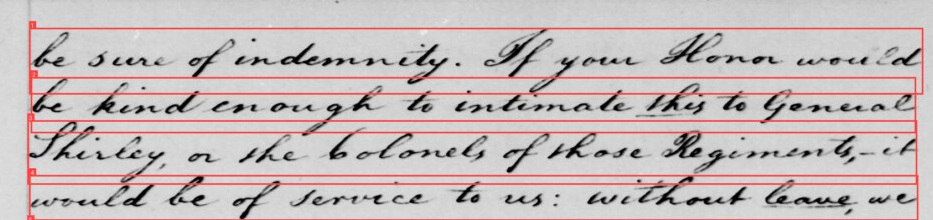
\includegraphics[width=\linewidth,height=0.16\textheight,keepaspectratio]{images/pdf_optimized/intro_washington_304_overlay_crop.jpg}
  \end{minipage}

  \vspace{0.45em}
  \begin{minipage}{0.96\linewidth}
    \textbf{2. Known transcription without task line breaks}
    \par\vspace{0.25em}
    \fbox{\begin{minipage}{0.975\linewidth}
      \raggedright\ttfamily
      be sure of idemnity. If your Honor would be kind enough to intimate this to General Shirley, or the Colonels of those Regiments,- it would be of service to us: without leave we
    \end{minipage}}
  \end{minipage}

  \vspace{0.45em}
  \begin{minipage}{0.96\linewidth}
    \textbf{3. Desired output with inserted newline markers}
    \par\vspace{0.25em}
    \fbox{\begin{minipage}{0.975\linewidth}
      \raggedright\ttfamily
      be sure of idemnity. If your Honor would \introNewlineMarker\\
      be kind enough to intimate this to General \introNewlineMarker\\
      Shirley, or the Colonels of those Regiments,- it \introNewlineMarker\\
      would be of service to us: without leave we
    \end{minipage}}
  \end{minipage}
  \caption{Line-level transcription alignment as boundary recovery with an already available transcription. The printed \texttt{\textbackslash n} markers denote task newlines, and ordinary line wrapping inside the figure is visual. Only newline characters may be inserted at the positions implied by the manuscript line structure; every other character in the supplied transcription is preserved, including the source spelling in the Washington Handwritten excerpt.}
  \label{fig:intro_newline_alignment_task}
\end{figure}

The example motivates the line-structure-first metrics used in Chapter~\ref{cha:experimentation}: The character stream can be correct while the recovered line structure is still wrong \thesiscite{vidal2023pageLevelAssessment,peer2025ctcBullingerAlignment}.

Prior work on document line processing typically evaluates segmentation, baseline detection, recognition, or task-specific alignment pipelines under their own input assumptions and error models \thesiscite{LombardiMarinai2020HDASurvey,likformansulem2006textLineSurvey,gruning2018readbad,fischer2011icdarInaccurateAlignment}. Recent LLMs and VLMs for document processing likewise focus mainly on OCR-free transcription, structured document parsing, or broader multimodal document understanding rather than on transcription alignment with a fixed transcription and a newline-only evaluation target \thesiscite{kim2022donut,nougat2023,wang2024docllm,wang2024qwen2vl}. As a result, direct evidence for LLM/VLM-based newline-only alignment in this constrained setting remains limited. They are worth evaluating here because they can combine visual, textual, and structural cues without first training a task-specific alignment model for each evidence setting. That flexibility also creates a validity problem: Generative outputs can copy, omit, normalize, or restructure text, so they must be checked against the fixed-transcription requirement. This thesis therefore evaluates LLM/VLM-based alignment as an empirical question about evidence, output control, and boundary accuracy rather than as a general claim about document understanding.

The documented comparison covers three implemented families under a shared newline-only evaluation target: LLM/VLM regimes that score raw returned text, LLM/VLM regimes that add structured output control before scoring, and NNTP as the deterministic token-passing forced-alignment baseline used here. The shorthand used for the five LLM/VLM-based regimes is Methods 1 to 5 (M1--M5); Chapter~\ref{cha:method} gives their operational definitions. NNTP provides the deterministic comparison point because it aligns a fixed transcription to recognizer-derived line evidence and inserts boundary positions rather than freely generating a new transcription \thesiscite{peer2025ctcBullingerAlignment}. The analysis therefore separates the observed relationship between input-evidence regimes and boundary accuracy from the separate validity question of whether LLM/VLM outputs can be made compatible with the newline-only target.

In this thesis, a \emph{regime} means the complete evaluated configuration, not only the named method or model. It includes the evidence supplied to the system, the output-control path, the provider or model setting where that affects the realized run, and the provenance of the artifacts that are actually scored.

Handwritten datasets form the main evaluation scope because line boundaries are especially difficult in handwriting and because many historical document collections are handwritten. In this thesis, that scope comprises Bullinger Handwritten, Children Handwritten, IAM Handwritten, and Washington Handwritten \thesiscite{Muehlberger2019TransformingScholarship,LombardiMarinai2020HDASurvey,likformansulem2006textLineSurvey,nikolaidou2022historicalDatasetSurvey}. The printed versions of Bullinger and IAM are included as additional context for the same newline-only task, not as a second full evaluation track. Bullinger Print and IAM Print therefore broaden the empirical setting for M1--M3, while the full M1--M5 plus NNTP comparison remains centered on handwriting.

\section{Research Questions}
\label{sec:intro_research_questions}

The problem statement leads to three Research Questions (RQs) that structure the remainder of the thesis. The mapping is focused: Input evidence and newline-boundary accuracy motivate RQ1; the deterministic forced-alignment comparison motivates RQ2; and output validity, repair, fallback, projection, and compatibility with the newline-only target motivate RQ3. In RQ2, NNTP is used as the deterministic forced-alignment baseline because its alignment step is constrained by the supplied transcription and recognizer evidence, while LLM/VLM-based regimes receive prompts and can initially generate, omit, normalize, or restructure text before any validation or projection step corrects them \thesiscite{peer2025ctcBullingerAlignment,geng2023grammar}. The questions therefore compare complete evaluated regimes; component isolation is treated later as an interpretation boundary.

\paragraph{RQ1.} Which input-evidence regimes most improve newline-boundary accuracy for fixed transcriptions?

\paragraph{RQ2.} How does the strongest reported LLM/VLM-based regime compare with NNTP, a deterministic forced-alignment baseline, under the same newline-only evaluation target?

\paragraph{RQ3.} To what extent do structured output control, repair, fallback, and projection make LLM/VLM outputs valid under the fixed-transcription newline-only requirement?

\section{Contribution and Scope}
\label{sec:intro_contribution_scope}

The thesis contributes five focused deliverables to the newline-only alignment problem:
\begin{itemize}
  \item A documented empirical benchmark of multiple evaluated LLM/VLM configurations for newline-only alignment on the main handwritten scope, with additional M1--M3 print context;
  \item A comparison of input-evidence regimes for recovering line boundaries under a fixed transcription;
  \item A structured output-control layer for testing whether model outputs can be made valid under the fixed-transcription newline-only requirement;
  \item A comparison with NNTP as a deterministic forced-alignment baseline under the same newline-only evaluation target;
  \item A reproducibility and validity evidence layer covering evaluation-version choice, dataset provenance, detailed validity conditions, output control, provider provenance, and NNTP preprocessing boundaries.
\end{itemize}

The scope is intentionally specific: The thesis assumes known text and evaluates how faithfully systems restore line structure under the newline-only constraint \thesiscite{fischer2011icdarInaccurateAlignment,kim2022donut}. Within that scope, M1--M5 and NNTP should be read as complete evaluated regimes rather than as isolated component tests. Method 5 is therefore interpreted as the strongest reported LLM/VLM-based regime under the evaluated context-rich structured configuration, while Chapter~\ref{cha:method} and Chapter~\ref{cha:experimentation} keep provider controls and component-level interpretation boundaries explicit.

\section{Structure}
\label{sec:intro_structure}

The remainder of the thesis is organised to keep problem definition, prior work, data, method description, and empirical evidence clearly separated. The chapter sequence moves from formal task definition and prior work to the evidence base, method comparison, and the empirical results that answer the three research questions.

\begin{itemize}
  \item Chapter~\ref{cha:theory_background} formalizes newline-only alignment, introduces the notation used throughout the thesis, and explains the LLM/VLM concepts needed for the method comparison.
  \item Chapter~\ref{cha:state_of_the_art} situates the work in prior research on document layout analysis, transcription alignment, and modern neural or multimodal document models.
  \item Chapter~\ref{cha:data} describes the handwritten evaluation datasets, the supporting print context, and the provenance of the \OCRHTR structural hints used by several methods.
  \item Chapter~\ref{cha:method} presents Methods 1 to 5, the benchmarked LLM/VLM model settings, NNTP as the deterministic forced-alignment baseline, and the surrounding \OCRHTR pipeline components.
  \item Chapter~\ref{cha:experimentation} defines the evaluation metrics, reports the LLM/VLM-based comparison on the four handwritten datasets, includes the additional M1--M3 print evaluation, presents the matched NNTP comparison on the datasets where that evidence is available, and includes the Bullinger published-baseline comparison with explicit version notes.
  \item Chapter~\ref{cha:conclusion} answers the three research questions, summarizes the main findings, and outlines the most important next steps for future work.
\end{itemize}

% Chapter 2 provides the minimal theory needed to understand newline-only alignment.
% Focus: problem formulation, what "a line" means in layout, recognition background,
% and conceptual LLM/VLM output-control background.
% Implementation-specific pipeline details belong to later chapters.

\chapter{Theory and Background}
\label{cha:theory_background}

Newline-only alignment sits close to handwriting recognition, page segmentation, and transcript alignment \thesiscite{fischer2011icdarInaccurateAlignment,hassner2013ocrFreeAlignment,vidal2023pageLevelAssessment}, but it follows a more specific task definition: The transcription remains fixed, and newline positions are predicted while keeping the character stream unchanged. This chapter therefore begins with the document-analysis setting, then introduces the formal notation, recognition concepts, and Large Language Model (LLM) / Vision-Language Model (VLM) output-control concepts needed later to compare regimes without changing that task definition.

\section{Document Analysis, Transcription, and Alignment}
\label{sec:theory_task_context}

Document analysis turns page images into usable structure: Text regions, reading order, line geometry, and eventually textual representations \thesiscite{Bulacu2007LayoutAnalysisCabinetQueen,binmakhashen2019dlaSurvey}. In historical and handwritten material, this is difficult because layout, degradation, writing style, and page conventions interact before any recognizer or downstream alignment method sees a clean sequence \thesiscite{likformansulem2006textLineSurvey}.

Transcription is the textual counterpart of that visual evidence. In OCR/HTR, the system usually has to recover the characters themselves from an image; in transcript alignment, a transcription is already available and the task is to connect that known text back to page evidence. Prior alignment systems therefore use the supplied transcript as a constraint while estimating how words, regions, or page evidence correspond to positions in the document image \thesiscite{tomai2002transcriptMapping,kornfield2004textAlignment,fischer2011icdarInaccurateAlignment,hassner2013ocrFreeAlignment}.

OCR/HTR output should therefore be treated as document evidence rather than as a perfect substitute for transcription. Recognition and segmentation systems can introduce content, ordering, or boundary errors in historical material \thesiscite{LombardiMarinai2020HDASurvey,vidal2023pageLevelAssessment}, while expert, editorial, or otherwise curated transcriptions may already encode the intended character sequence at a chosen level of detail \thesiscite{DriscollLevelsTranscription}. Newline-only alignment is useful in this situation because it treats the available transcription as the trusted character stream and recovers the line structure that connects it back to the page \thesiscite{tomai2002transcriptMapping,hassner2013ocrFreeAlignment}.

Line-level alignment is useful because many scholarly and technical workflows need more than a page-level text string. Lineation connects a transcription to image crops, supports inspection of local errors, preserves reading-order structure, and lets evaluation distinguish content recognition errors from structural line-placement errors. Page-level HTR assessment and historical line-detection protocols already show that text content, ordering, and line structure can fail in different ways; newline-only alignment isolates the text-side boundary placement part of that problem \thesiscite{gruning2018readbad,vidal2023pageLevelAssessment}.

\section{Document Layout and Text Lines}
\label{sec:theory_layout_lines}

In document analysis, a ``text line'' is not a single object type but a stack of related representations used at different stages of processing. At least three views are operationally relevant: A \emph{baseline} (a curve approximating where characters rest), a \emph{line region} (pixels or polygons containing ascenders and descenders around that baseline), and a \emph{logical line unit} in reading order (a sequence element in a transcription) \thesiscite{likformansulem2006textLineSurvey,gruning2018readbad}.

\paragraph{Baseline view.}
Baseline-centered formulations encode each line as a polyline rather than a full mask, which makes annotations compact and robust to moderate stroke thickness variation. This representation is dominant in historical baseline-detection benchmarks and is directly tied to tolerance-aware matching schemes for slightly displaced predictions \thesiscite{gruning2018readbad,gruning2019twoStageTextLine}.

\paragraph{Region view.}
Region-oriented formulations treat a line as a 2D support set (rectangle, polygon, or binary mask). This is convenient for crop extraction and recognition pre-processing, but boundaries become sensitive to script style, ascender/descender overlap, and local skew, so two systems can disagree on region contours while remaining semantically close \thesiscite{likformansulem2006textLineSurvey,diem2013textLineDetection}.

\paragraph{Logical-sequence view.}
For transcription and downstream Natural Language Processing (NLP), a line is an ordered textual unit. Here, the key question is not only ``which pixels belong together'' but also ``where this unit appears in reading order'' relative to neighboring lines or blocks, especially under multi-column layouts or marginal additions \thesiscite{binmakhashen2019dlaSurvey,vidal2023pageLevelAssessment}.

\paragraph{Why line boundaries matter.}
Line boundaries are the smallest structural decisions that connect a continuous transcription stream to the visual line units of a page. If a boundary is misplaced, the character sequence may still be correct while the recovered line sequence, crop correspondence, and local error attribution become wrong. This is why the thesis treats boundary placement as its own object of evaluation rather than as a side effect of page-level recognition quality \thesiscite{fischer2011icdarInaccurateAlignment,vidal2023pageLevelAssessment}.

\paragraph{Why boundaries are ambiguous.}
Historical pages often contain curved writing, touching components across adjacent lines, nonuniform spacing, bleed-through, and degradation. Under these conditions, multiple nearby separators can each be plausible, and split/merge decisions are partly convention-dependent rather than uniquely determined by local pixels \thesiscite{likformansulem2006textLineSurvey,gruning2019twoStageTextLine}.

Ambiguity also appears at annotation level: Different ground-truth policies may differ on whether short interlinear marks, ornaments, or marginal notes belong to a main line, a separate line, or no line at all. Competition protocols therefore use geometry-aware matching with tolerance rather than exact point coincidence, reflecting that ``line correctness'' is graded rather than strictly binary at page level \thesiscite{diem2017cbad,gruning2018readbad}.

For this thesis, these ambiguities motivate a focused operational choice: Line structure is represented only by newline insertion points in a fixed character stream, as formalized in \autoref{sec:theory_problem_definition}. This preserves a single textual sequence while making line hypotheses explicit as boundary decisions, without committing to one specific pixel-level line geometry \thesiscite{fischer2011icdarInaccurateAlignment,vidal2023pageLevelAssessment}.

\section{Problem Definition and Notation}
\label{sec:theory_problem_definition}

The formal definition below treats line-structure recovery as a constrained segmentation task over a known transcription stream. Prior document analysis work typically recovers line structure through visual line detection and structural alignment, especially in heterogeneous historical material where robust line geometry estimation is difficult \thesiscite{likformansulem2006textLineSurvey,fischer2011icdarInaccurateAlignment}.

Let $\Sigma$ denote the character alphabet excluding the newline token $\texttt{\textbackslash n}$. For one sample, let
\[
x=(x_1,\dots,x_n)\in\Sigma^n
\]
be the supplied transcription without line breaks. A line-break hypothesis is represented by a boundary vector
\[
b=(b_1,\dots,b_{n-1})\in\{0,1\}^{n-1},
\]
where $b_i=1$ means ``insert a newline after character $x_i$''.

Define the insertion operator $\mathcal{I}$ as
\begin{equation}
\mathcal{I}(x,b)=x_1\eta_1x_2\eta_2\cdots x_{n-1}\eta_{n-1}x_n,\qquad
\eta_i=
\begin{cases}
\texttt{\textbackslash n}, & b_i=1,\\
\epsilon, & b_i=0.
\end{cases}
\label{eq:newline_insertion_operator}
\end{equation}
Let $\pi(\cdot)$ remove all newline tokens. The newline-only constraint is
\begin{equation}
\pi\!\left(\mathcal{I}(x,b)\right)=x,
\label{eq:newline_projection_constraint}
\end{equation}
which enforces that character identity and order are unchanged.

The feasible output set induced by the boundary-vector representation is therefore
\begin{equation}
\mathcal{Y}(x)=\left\{\mathcal{I}(x,b)\mid b\in\{0,1\}^{n-1}\right\}.
\label{eq:feasible_set}
\end{equation}
This is the ideal newline-only task space. Raw prompt generations, by contrast, may temporarily occupy the broader string space $(\Sigma\cup\{\texttt{\textbackslash n}\})^\star$ before parser-side validation or projection maps them back to a boundary plan.
Given conditioning evidence $c$ (method-dependent in \autoref{cha:method}), an ideal boundary selector predicts
\begin{equation}
\hat{b}=\arg\max_{b\in\{0,1\}^{n-1}} p_\theta(b\mid x,c),\qquad
\hat{y}=\mathcal{I}(x,\hat{b}).
\label{eq:boundary_prediction_objective}
\end{equation}
This notation is a conceptual formalization of preference over boundary plans under conditioning evidence. For the LLM/VLM-based regimes M1--M5, it should not be read as a claim that the implementation explicitly estimates a calibrated probability distribution over boundary vectors; the implemented systems instead generate outputs and then parse, validate, repair, or project them as described in Chapter~\ref{cha:method}. More generally, \autoref{eq:boundary_prediction_objective} is literal only for methods that actually score candidate boundary plans in that form.
In the implemented thesis method set, this abstract conditioning variable expands to the high-level bundles
\[
\begin{aligned}
c_{\mathrm{M1}}&=(v,x), &
c_{\mathrm{M2}}&=(v,o,x), &
c_{\mathrm{M3}}&=(o,x), \\
c_{\mathrm{M4}}&=(s,N,x), &
c_{\mathrm{M5}}&=(g,s,p,N,x), &
c_{\mathrm{NNTP}}&=(g,\lambda,x),
\end{aligned}
\]
where $v$ denotes ordered page-image evidence, $o$ Optical Character Recognition / Handwritten Text Recognition (OCR/HTR) text, $s$ an ordered OCR-line scaffold, $g$ ordered line-image crops, $p$ page-level visual context, $N$ the expected line count, and $\lambda$ recognizer-side line observations used by NNTP. For M5, $s$ denotes the structured line record from which both the ordered crop references and the OCR/HTR line text are available; in the evaluated M5 configuration, that OCR/HTR line text and page-level visual context are supplied as secondary evidence around the primary line-image anchors. For NNTP, $\lambda$ should be read as Connectionist Temporal Classification (CTC)-style line evidence produced by an HTR recognizer and consumed by a forced-alignment algorithm; the algorithm searches for boundary placements under the fixed transcription rather than sampling or generating a rewritten string, in line with the Bullinger CTC alignment baseline \thesiscite{peer2025ctcBullingerAlignment}. Chapter~\ref{cha:method} makes the provenance of these artifacts explicit; most importantly for later interpretation, $N$ is supplied to M4 and M5 from stored OCR-line metadata in the evaluated handwritten datasets rather than predicted from page evidence.

Across all regimes, the output target and constraint remain fixed: Only newline boundaries are predicted while character content is preserved.

This makes the task a structured insertion problem in the specific thesis sense: Generate only separators while preserving the source sequence.

The boundary vector induces a line segmentation. Let
\[
0=t_0<t_1<\cdots<t_m=n
\]
with $b_{t_j}=1$ for $j=1,\dots,m-1$. The reconstructed lines are contiguous spans
\begin{equation}
\ell_j = x_{(t_{j-1}+1):t_j},\qquad j=1,\dots,m,\qquad
m=1+\sum_{i=1}^{n-1} b_i.
\label{eq:induced_lines}
\end{equation}
Hence the newline-only alignment problem is equivalent to predicting the ordered set of split indices.

\paragraph{Toy example.}
Let $x=\texttt{ABCDEFG}$ and $b=(0,1,0,0,1,0)$. Then
\[
\hat{y}=\mathcal{I}(x,b)=\texttt{AB\textbackslash nCDE\textbackslash nFG},
\]
with induced lines $(\texttt{AB},\texttt{CDE},\texttt{FG})$. This example illustrates that only boundary positions change; the underlying character sequence remains fixed.

Figure~\ref{fig:theory_newline_only_schematic} gives the same newline-only insertion logic as a compact schematic: The fixed transcription stays unchanged, the boundary vector marks split positions, and the insertion operator produces the ordered line sequence.

\begin{figure}[H]
  \centering
  \begin{tikzpicture}[
    font=\scriptsize,
    >={Latex[length=2mm]},
    box/.style={rectangle, rounded corners=2pt, draw=black, thick, align=left, inner sep=6pt, text width=0.84\linewidth},
    flow/.style={->, thick}
  ]
    \node[box, fill=gray!10] (xbox) {\textbf{Fixed transcription} \(x=\texttt{ABCDEFGH}\)};
    \node[box, fill=blue!8, below=0.55cm of xbox] (bbox) {\textbf{Boundary vector} \(b=(0,1,0,1,0,1,0)\)\\Insert a newline after characters \(2,4,6\).};
    \node[box, fill=orange!12, below=0.55cm of bbox] (ibox) {\textbf{Insertion operator} \(\mathcal{I}(x,b)=\texttt{AB\textbackslash nCD\textbackslash nEF\textbackslash nGH}\)};
    \node[box, fill=green!10, below=0.55cm of ibox] (lbox) {\textbf{Induced line sequence} \((\texttt{AB},\texttt{CD},\texttt{EF},\texttt{GH})\)};
    \draw[flow] (xbox) -- (bbox);
    \draw[flow] (bbox) -- (ibox);
    \draw[flow] (ibox) -- (lbox);
  \end{tikzpicture}
  \caption{Schematic of the newline-only task. The character stream stays fixed and only the boundary vector changes, so the operator \(\mathcal{I}\) inserts line breaks without rewriting the transcription.}
  \label{fig:theory_newline_only_schematic}
\end{figure}


% Note: implementation-specific OCR/HTR pipeline details are described in later chapters (Method/Experimentation).

\section{Encoder--Decoder Recognition Background}
\label{sec:theory_encoder_decoder}

This section summarizes recognition architectures that appear as auxiliary components in document pipelines. Given a line image $I$, recognition predicts a character sequence
\[
\hat{y}=\arg\max_{y} p_\phi(y\mid I).
\]
In modern OCR/HTR, two families are central for this mapping: Connectionist Temporal Classification (CTC)-based recognizers and encoder--decoder recognizers with attention \thesiscite{graves2006ctc,li2023trocr}.

\paragraph{Connectionist Temporal Classification (CTC)-based recognition.}
Let an encoder produce a feature sequence $h_{1:T}=f_{\text{enc}}(I)$. CTC introduces an alignment space over $\Sigma\cup\{\varnothing\}$ (blank symbol) and defines
\begin{equation}
p(y\mid I)=\sum_{\pi\in\mathcal{B}^{-1}(y)}\prod_{t=1}^{T} p(\pi_t\mid h_t),
\label{eq:ctc_objective}
\end{equation}
where $\mathcal{B}$ collapses repeated labels and blanks. This yields alignment-free training under a monotonic left-to-right assumption and is widely used in HTR baselines \thesiscite{graves2006ctc,puigcerver2017icdar}.

\paragraph{Encoder--decoder attention recognition.}
Encoder--decoder models factorize the output autoregressively as
\begin{equation}
p(y\mid I)=\prod_{i=1}^{|y|} p(y_i\mid y_{<i},h_{1:T}),
\label{eq:enc_dec_objective}
\end{equation}
with a decoder that conditions on previous tokens and attends to encoder features through cross-attention. Transformer instantiations use masked self-attention in the decoder and multi-head cross-attention to visual states \thesiscite{vaswani2017transformer,li2023trocr}.

\paragraph{TrOCR as an OCR/HTR example.}
TrOCR instantiates this design with a vision encoder and a Transformer text decoder, pretrained on large synthetic corpora and then fine-tuned on downstream OCR/HTR datasets. The model therefore combines visual representation learning with autoregressive token generation in a single sequence-to-sequence objective \thesiscite{li2023trocr}.

\paragraph{CTC vs encoder--decoder: Practical trade-off.}
CTC provides a strong monotonic alignment prior and non-autoregressive frame scoring. Encoder--decoder systems instead model output-token dependencies explicitly through decoder state and cross-attention. In practice, this yields a trade-off between simpler decoding assumptions (CTC) and richer sequence modeling with sequential inference cost (encoder--decoder) \thesiscite{graves2006ctc,li2023trocr}.

For this thesis, recognition is background context rather than the main prediction target: The evaluated newline-only alignment task predicts newline positions while keeping the character stream fixed (\autoref{sec:theory_problem_definition}). Recognition outputs are relevant when OCR/HTR is used as auxiliary structural evidence in later methods, not as the primary quantity to be generated. In NNTP-style CTC transcription alignment, these recognition outputs become posterior evidence for a deterministic token-passing or dynamic-programming alignment step that places the known transcription against line images and recovers newline positions \thesiscite{fischer2011icdarInaccurateAlignment,li2023trocr,peer2025ctcBullingerAlignment}.

\section{LLM/VLM Basics for Constrained Structured Output}
\label{sec:theory_llm_vlm_structured_output}

Large Language Models (LLMs) and Vision-Language Models (VLMs) are useful background for this thesis because all five LLM/VLM-based regimes ask a general-purpose model to infer line breaks from textual or visual evidence. At the architectural level, most current systems are built from Transformer blocks. A Transformer represents an input sequence through self-attention: Each token can weight information from other tokens, and multi-head attention lets the model combine several such relations in parallel. This made it possible to train sequence models without recurrence or convolution as the central sequence mechanism, and it remains the standard conceptual basis for modern language and multimodal decoders \thesiscite{vaswani2017transformer}.

An autoregressive language model generates text one token at a time. At decoding step \(t\), the next token is predicted from the already generated prefix and the conditioning input:
\[
p(y\mid u)=\prod_{t=1}^{|y|}p(y_t\mid y_{<t},u).
\]
For a text-only LLM, \(u\) may be the prompt and any supplied transcription. For a VLM, \(u\) can additionally include image-derived representations that are connected to the text decoder through cross-attention or related multimodal fusion mechanisms. OCR/HTR encoder--decoder systems such as TrOCR instantiate the same basic sequence-to-sequence idea at document scale: A visual encoder represents the image and a Transformer decoder produces the text sequence autoregressively \thesiscite{vaswani2017transformer,li2023trocr}.

Document-understanding models extend this setup because document images contain more than word identity. Layout, reading order, regions, tables, handwriting style, and local image evidence all influence the intended output. Layout-aware and OCR-free models therefore combine visual appearance, textual tokens, and spatial or structural cues in different ways. Donut, for example, maps document images directly to structured textual outputs without a separate OCR stage, while LayoutLMv3 and DocLLM represent document-specific text, image, and layout information for downstream document tasks. These models motivate using multimodal evidence for line-structure recovery, but their usual task definition is broader than the one studied here because they often generate or classify content rather than preserving a supplied transcription exactly \thesiscite{kim2022donut,huang2022layoutlmv3,wang2024docllm}.

The exact-preservation requirement is the central difficulty for applying generative models to newline-only alignment. A prompt can ask a model to ``copy this text and add line breaks'', but autoregressive decoding still chooses each output token from a large vocabulary, and LLM performance can be sensitive to the requested output format even when task content is otherwise unchanged. In this setting, a malformed response may normalize spelling, alter punctuation, omit a repeated word, repair what looks like an OCR error, or introduce visually plausible text that is not present in the fixed transcription \thesiscite{ravikumar2026lostFormatting,liu2024ocrbench}. Such behavior can be useful in open transcription or correction tasks, but it violates the feasible set \(\mathcal{Y}(x)\) in \autoref{eq:feasible_set}: For this thesis, the text is already fixed and only separator positions may change.

This makes the thesis task a form of constrained generation or constrained sequence segmentation. The admissible output is not any fluent string; it is a boundary plan \(b\in\{0,1\}^{n-1}\) over a known character stream. In an ideal token-level constrained decoder, decoding could be restricted to
\begin{equation}
\hat{y}=\arg\max_{y\in\mathcal{C}(u)} p_\theta(y\mid u),
\label{eq:generic_constrained_decoding}
\end{equation}
where \(u\) is the text-only or multimodal input and \(\mathcal{C}(u)=\mathcal{Y}(x)\). This separates the model's preference over likely outputs from the hard validity rule that the non-newline character sequence must stay unchanged. Work on structured outputs and constrained decoding treats such output validity as a first-class problem, often using grammars, schemas, token masks, or post-generation validation to keep generated text inside a target format \thesiscite{geng2023grammar,geng2025jsonschemabench}.

Insertion-based generation is conceptually close to the newline-only formulation because it begins with an existing canvas and inserts material into it \thesiscite{stern2019insertionTransformer,zhang2020pointer}:
\begin{equation}
y^{(t+1)}=\operatorname{Insert}\!\left(y^{(t)}, c_t, \ell_t\right),
\label{eq:insertion_update}
\end{equation}
where token \(c_t\) is inserted at location \(\ell_t\) in the current sequence. The thesis does not implement an insertion Transformer, but the abstraction is helpful: Newline-only alignment is the special case where the only insertable token is \(\texttt{\textbackslash n}\), and all original characters must remain in order. This is why validation, repair, fallback, and projection matter. They convert an unconstrained or weakly constrained model response into an inspectable boundary plan, or reject it when the response cannot be reconciled with the fixed transcription.

The distinction between prompted generation and deterministic or forced-alignment approaches follows from this output-validity requirement. LLM/VLM-based regimes ask a model to infer the line structure from instructions plus evidence such as page images, OCR/HTR text, ordered OCR lines, or line crops; unless additional checks are applied, their first output is still a generated string that may omit, normalize, or restructure the supplied text. Deterministic or forced-alignment approaches instead treat the known transcription as a constraint from the start and align recognizer or image-derived observations to that fixed sequence \thesiscite{fischer2011icdarInaccurateAlignment,hassner2013ocrFreeAlignment,peer2025ctcBullingerAlignment}. The former family tests whether a general-purpose generative model can use rich context and satisfy that validity requirement; the latter supplies a non-prompt baseline whose errors are more directly tied to alignment evidence and preprocessing assumptions.

% Chapter 3 positions newline-only alignment against prior work on
% layout analysis, transcript alignment, OCR/HTR pipelines, and modern document models.
% The emphasis is analytical positioning rather than an exhaustive survey of OCR or VLM research.

\chapter{Related Work and Positioning}
\label{cha:state_of_the_art}

Document-processing methods are difficult to compare when they solve different task definitions. The related-work discussion positions newline-only alignment against neighboring fields rather than attempting an exhaustive survey of Optical Character Recognition (OCR), Handwritten Text Recognition (HTR), Large Language Model (LLM), or Vision-Language Model (VLM) research. The main organizing question is which prior families share the thesis input/output assumptions: A fixed transcription, line-boundary recovery as the central objective, and evaluation that separates structural error from lexical error \thesiscite{fischer2011icdarInaccurateAlignment,hassner2013ocrFreeAlignment,vidal2023pageLevelAssessment}. Broad document-processing work remains important context, but it is directly comparable only when those assumptions are similar.

\section{Task Definitions in Prior Work}
\label{sec:sota_task_definitions}

Prior work on line structure can be organised more clearly by \emph{task definition} than by model chronology alone. The key dimensions for this thesis are whether the transcription is fixed or must still be recognized, whether the expected line count is inferred or externally scaffolded, whether structure is predicted geometrically on the image side or inserted as newlines on the text side, whether inference uses deterministic alignment or prompted model generation, and whether the output is constrained to preserve known text. These dimensions determine whether a method is a direct comparator, a close predecessor under broader alignment assumptions, or contextual background \thesiscite{fischer2011icdarInaccurateAlignment,kim2022donut,wang2024docllm}.

\begin{table}[t]
    \centering
    \scriptsize
    \setlength{\tabcolsep}{2.5pt}
    \renewcommand{\arraystretch}{1.08}
    \caption{Task-definition view of prior-work families relevant to newline-only alignment, with representative sources for each family.}
    \label{tab:sota_task_definitions}
    \begin{tabularx}{\linewidth}{@{}>{\raggedright\arraybackslash}p{0.17\linewidth}>{\raggedright\arraybackslash}p{0.18\linewidth}>{\raggedright\arraybackslash}p{0.18\linewidth}>{\raggedright\arraybackslash}p{0.20\linewidth}Y@{}}
        \toprule
        Prior-work family & Representative sources & Transcription / output assumptions & Main structure strategy & Difference from this thesis \\
        \midrule
        Layout analysis / page segmentation &
        \thesiscite{Bulacu2007LayoutAnalysisCabinetQueen,xu2018multitaskLayoutAnalysis,binmakhashen2019dlaSurvey} &
        No fixed transcription; output is page geometry or logical regions &
        Detect regions, reading order, and separators on the image side &
        Context only: Recovers page structure before text-side newline insertion \\
        \addlinespace[0.2em]
        Baseline detection / text-line segmentation &
        \thesiscite{likformansulem2006textLineSurvey,rabaev2026textLineSegmentationReview,gruning2018readbad} &
        No fixed transcription; output is line or baseline geometry &
        Localize line geometry on the image side &
        Context only: Estimates latent line structure, but does not insert newlines into known text \\
        \addlinespace[0.2em]
        Transcript alignment / forced alignment &
        \thesiscite{tomai2002transcriptMapping,kornfield2004textAlignment,rothfeder2006aligningTranscripts,fischer2011icdarInaccurateAlignment} &
        Known transcript constrains alignment; output links text units to image evidence &
        Transfer image-side word, region, or page correspondences onto transcript positions &
        Direct predecessor: Shares the known-transcript assumption, but the thesis restricts output to a newline-boundary vector \\
        \addlinespace[0.2em]
        Modular OCR/HTR pipelines &
        \thesiscite{marti2001statisticalLanguageModelHMM,puigcerver2017icdar,li2023trocr} &
        Recognize text from segmented images; output characters or words are not fixed in advance &
        Detect lines first, then recognize text per line or crop &
        Useful evidence source for this thesis, but standard scores mix recognition and structure errors \\
        \addlinespace[0.2em]
        End-to-end page transcription models &
        \thesiscite{wigington2018sfr,coquenet2023dan,kim2022donut} &
        Generate page or paragraph text; line count and text content emerge during decoding &
        Learn recognition and structure jointly or implicitly &
        Context only: Mixes content recovery with structural formatting instead of fixing the character sequence \\
        \addlinespace[0.2em]
        Layout-aware document models &
        \thesiscite{huang2022layoutlmv3,wang2024docllm,wang2024qwen2vl} &
        Usually consume OCR/layout cues or multimodal inputs for document-understanding outputs &
        Use multimodal structure cues for downstream labels or structured output &
        Contextual neighbor: Shares layout evidence types, but not the fixed-transcription newline-only target \\
        \addlinespace[0.2em]
        LLM/VLM prompting / formatting &
        \thesiscite{mathew2021docvqa,liu2024ocrbench,wang2024qwen2vl} &
        Prompt-conditioned generation; preservation of supplied text is requested or checked externally &
        Generate formatted text from page images and prompts &
        Adapted in the LLM/VLM-based regimes, but broad benchmark results remain contextual unless output is projected to newline-only form \\
        \bottomrule
    \end{tabularx}
\end{table}

\noindent \autoref{tab:sota_task_definitions} makes explicit why broad OCR or VLM results should not be read as direct baselines for this thesis. As soon as a method is still responsible for recovering unknown text, inferring its own line count implicitly, or generating unconstrained output, content error and line-structure error become entangled. The thesis instead fixes the non-newline character sequence and evaluates only where newline boundaries are placed. Layout analysis, baseline detection, OCR/HTR pipelines, and document foundation models remain informative mainly as neighboring evidence regimes or upstream structure providers, while transcript alignment is the closest prior task family \thesiscite{kornfield2004textAlignment,fischer2011icdarInaccurateAlignment,hassner2013ocrFreeAlignment,kim2022donut,wang2024docllm}.

\section{Transcription Alignment and Forced Alignment}
\label{sec:sota_transcription_alignment}

The closest task family and direct predecessor is transcript alignment, especially work that maps known transcripts to handwritten page evidence without requiring line breaks in the supplied text. That family already shares the known-transcript alignment assumptions; the specific contribution here is to collapse the admissible output to newline positions in a fixed character stream rather than to the richer word-image, region-image, or page-image correspondences usually produced by alignment systems \thesiscite{kornfield2004textAlignment,fischer2011icdarInaccurateAlignment,hassner2013ocrFreeAlignment}.

Once a transcription is known, the central question becomes how image-derived line evidence is transferred back onto text positions. Early handwritten-document transcript mapping and dynamic time warping / hidden Markov model alignment work already treats the transcription as a constraining object rather than as text to be recognized from scratch \thesiscite{tomai2002transcriptMapping,kornfield2004textAlignment,rothfeder2006aligningTranscripts}. Fischer \etal formulate this as forced alignment under recognition uncertainty, using hidden Markov model correspondence between transcript elements and page evidence \thesiscite{fischer2011icdarInaccurateAlignment,fischer2011latinManuscriptsHMM}; Hassner \etal pursue OCR-free transcript alignment directly against the document image \thesiscite{hassner2013ocrFreeAlignment}. In these cases, the transcription is no longer generated freely, and the task shifts from recognizing content to placing known content correctly against visual structure.

This bridge from geometry to transcript positions is exactly where the thesis methods enter. The thesis focuses the established alignment assumptions further: The character sequence is fixed, only newline separators may be inserted, and alternative evidence regimes are compared under one downstream metric family. This restriction makes line-structure recovery analyzable without attributing lexical substitutions, deletions, or hallucinated insertions to the same score. It also limits the novelty claim: Transcript alignment and known-transcript forced alignment are not new tasks, and prior systems already align supplied text to page evidence \thesiscite{kornfield2004textAlignment,fischer2011icdarInaccurateAlignment,hassner2013ocrFreeAlignment}. What is more specific here is the output representation and evaluation target: Richer word-image, region-image, or page-image correspondences are reduced to an isolated newline-boundary vector over a fixed transcription. \needspace{4\baselineskip}The result is a controlled evaluation problem rather than a claim that known-transcript alignment itself is new.

\section{Layout Analysis and Line Segmentation as Upstream Tasks}
\label{sec:sota_layout_upstream}

Classical document layout analysis and text-line segmentation provide the image-side half of the problem. Page segmentation methods decompose documents into blocks, columns, and reading order \thesiscite{Bulacu2007LayoutAnalysisCabinetQueen,xu2018multitaskLayoutAnalysis,binmakhashen2019dlaSurvey,ha1995recursiveXYCut,shafait2008benchmarkingSeg}, while handwritten-text research concentrates on line and baseline extraction under skew, curvature, overlap, and degradation \thesiscite{likformansulem2006textLineSurvey,rabaev2026textLineSegmentationReview,gruning2018readbad}. These families are highly relevant because they estimate the latent line structure that any later alignment method must exploit. Their native evaluation protocols, however, score geometric objects such as regions, separators, or baselines rather than newline placement in a fixed transcription \thesiscite{clausner2011scenarioDrivenEval,gruning2018readbad}.

The upstream relation matters for the thesis methods because several regimes use structural evidence produced before newline insertion: Page images, OCR/HTR text, ordered OCR lines, expected line counts, and line-image crops. Layout-analysis and line-segmentation systems are therefore not direct newline-only baselines, but they define the evidence types and error sources that a text-side alignment method inherits \thesiscite{Bulacu2007LayoutAnalysisCabinetQueen,likformansulem2006textLineSurvey,gruning2018readbad}.

\section{Encoder--Decoder and Sequence-Based Neural Document Processing}
\label{sec:sota_sequence_neural}

Modern neural pipelines still often preserve an explicit structure-recognition interface. Systems built from line detectors or segmenters plus recognizers such as Kraken, docTR, or TrOCR make line evidence operational and reusable, but they also expose the thesis-relevant dependency that segmentation mistakes propagate into any downstream text transfer step. For the present thesis, such systems matter less as direct benchmarks than as sources of structured evidence regimes: Page images alone, \OCRHTR text, ordered OCR lines, or line-image crops. Their ordinary objective is still recognition, whereas the thesis objective begins after the transcription has been fixed \thesiscite{marti2001statisticalLanguageModelHMM,puigcerver2017icdar,kiessling2025kraken,mindee2026doctr,li2023trocr}.

Other neural work pushes line structure inside the recognizer. Start, Follow, Read and Document Attention Network (DAN) reduce the explicit interface between line detection and transcription by letting attention or sequence modeling absorb more of the ordering problem. These systems are important context because they show how sequence models can combine recognition and structure, but their standard objectives usually evaluate content recovery and structure recovery together rather than isolating newline placement over a fixed transcription \thesiscite{wigington2018sfr,coquenet2023dan,kim2022donut}.

\section{LLM/VLM-Based Document Processing and Structured Output}
\label{sec:sota_llm_vlm_structured}

Document foundation models extend neural document processing by combining visual appearance, text, layout, and task instructions. LayoutLMv3 learns joint text-image representations, Donut and Nougat generate document text or markup directly from page images, and DocLLM or general-purpose VLMs operate over mixed textual, spatial, and visual cues. These systems are important context because they demonstrate strong multimodal priors, but their standard evaluations usually combine content recovery, structure recovery, and task-specific formatting into one broader objective \thesiscite{huang2022layoutlmv3,kim2022donut,nougat2023,wang2024docllm,wang2024qwen2vl}.

That distinction matters for claims of comparability. OCR-heavy and VLM-heavy benchmarks document useful failure modes, especially on handwriting, non-semantic text, and layout-sensitive reasoning, but they do not usually ask whether a known transcription can be restored to the correct lineation without changing its character content. Their results should therefore be read as contextual evidence about the strengths and weaknesses of modern document models, not as direct state-of-the-art numbers for newline-only alignment \thesiscite{liu2024ocrbench,mathew2021docvqa,wang2024qwen2vl}.

Structured-output and constrained-decoding work is relevant because the LLM/VLM-based regimes in this thesis ask a generative model to produce a string that must remain valid under a hard preservation rule. Grammars, schemas, token masks, validation, repair, and projection all address the same general problem of keeping generated text inside an admissible output space, although the thesis applies that idea to newline insertion rather than to a general document-understanding schema \thesiscite{geng2023grammar}.

\section{Deterministic Baselines and Evaluation Differences}
\label{sec:sota_deterministic_baselines}

Deterministic forced-alignment baselines are relevant in this thesis because they operationalize the fixed-transcription assumption under stronger output control than free generation \thesiscite{fischer2011icdarInaccurateAlignment,hassner2013ocrFreeAlignment,peer2025ctcBullingerAlignment}. When line hypotheses, OCR-derived anchors, or recognizer-side alignments are converted into newline decisions without allowing arbitrary text rewriting, errors can be interpreted more cleanly as failures of structure transfer rather than of open-ended decoding. LLM/VLM-based regimes are different: They can combine visual, textual, and instruction-level evidence flexibly, but their raw decoder output is a string-generation process whose validity must be requested, checked, repaired, or projected after generation \thesiscite{geng2023grammar}. NNTP-style CTC alignment belongs to the forced-alignment side of this divide: It uses recognizer posteriors and dynamic programming over a fixed transcription to recover line boundaries, so it does not create new lexical content \thesiscite{graves2006ctc,peer2025ctcBullingerAlignment}. This makes deterministic baselines analytically valuable even when their upstream evidence differs from LLM/VLM-based regimes: They help separate the effect of scaffolding from the effect of unconstrained generation.

Within the method set of this thesis, that is why NNTP is not just an engineering baseline but a positioning device. It continues the transcript-alignment tradition by preserving the downstream focus on correspondence and boundary placement, while the LLM/VLM-based regimes M1--M5 show what happens when the same problem is delegated to increasingly structured multimodal generation. The comparison is bounded in ways the method and experimentation chapters make explicit: Recognizer-specific preprocessing, staged line-image inventories, and denominator availability affect how directly NNTP rows can be compared with the LLM/VLM rows. Even with those qualifications, a deterministic forced-alignment baseline remains the most informative non-prompt anchor for interpreting whether improvements come from stronger structural evidence, stronger output control, or broader generative capability \thesiscite{fischer2011icdarInaccurateAlignment,hassner2013ocrFreeAlignment,peer2025ctcBullingerAlignment}.

\enlargethispage{4\baselineskip}
Quantitative prior work is fragmented because different families score different objects. Baseline competitions measure geometric localization; transcript-alignment studies come closer to text-to-line correspondence but still use their own task definitions; and page-level HTR assessment separates content and order effects without turning newline insertion into the primary prediction target. Reported numbers are therefore best treated as protocol-specific context rather than as a single cross-paper leaderboard \thesiscite{diem2017cbad,gruning2018readbad,degregorio2023moccia,vidal2023pageLevelAssessment}.

\begin{table}[H]
    \centering
    \footnotesize
    \setlength{\tabcolsep}{3pt}
    \renewcommand{\arraystretch}{1.02}
    \caption{Representative quantitative context for line-structure quality. Values remain informative within their original protocols, not as one shared newline-only benchmark.}
    \label{tab:sota_line_baseline_landscape}
    \begin{tabular}{@{}>{\raggedright\arraybackslash}p{0.21\linewidth}>{\raggedright\arraybackslash}p{0.16\linewidth}>{\raggedright\arraybackslash}p{0.22\linewidth}>{\raggedright\arraybackslash}p{0.31\linewidth}@{}}
        \toprule
        Work / protocol family & Scored object & Representative reported result & Why it is not a thesis-style newline benchmark \\
        \midrule
        cBAD baseline detection competition \thesiscite{diem2017cbad} &
        Baseline $P/R/F$ &
        $F=0.971$ (simple); $F=0.859$ (complex) &
        Measures geometric localization only; it does not transfer a fixed transcription into newline positions \\
        \addlinespace[0.2em]
        READ-BAD baseline detection \thesiscite{gruning2018readbad} &
        Baseline $P/R/F$ &
        $F=0.912$ (simple); $F=0.728$ (complex) &
        Scores historical baseline geometry under tolerance-based matching, not text-side boundary insertion \\
        \addlinespace[0.2em]
        End-to-end transcript alignment (Moccia Code) \thesiscite{degregorio2023moccia} &
        Line segmentation and alignment accuracy &
        92\% correctly segmented lines; $>$68\% alignment accuracy &
        Closest transcript-to-line comparator, but still defined on a different alignment protocol and metric set \\
        \addlinespace[0.2em]
        Page-level HTR assessment \thesiscite{vidal2023pageLevelAssessment} &
        Word Error Rate (WER), bWER/hWER, NSFD &
        No single line-break score &
        Useful because it separates content and ordering effects, but it still does not score newline insertion directly \\
        \bottomrule
    \end{tabular}
\end{table}

\noindent The main use of \autoref{tab:sota_line_baseline_landscape} is therefore interpretive: Prior quantitative evidence either evaluates geometry, correspondence under another task definition, or broader recognition tasks. The thesis contribution is more specific and more controlled. LLM/VLM-based regimes and deterministic alignment baselines are compared under one fixed-transcription, newline-only target, with line accuracy as the primary outcome and precision, recall, and raw/normalized Character Error Rate (CER) and Word Error Rate (WER) variants used as supporting diagnostics in \autoref{cha:experimentation} \thesiscite{degregorio2023moccia,vidal2023pageLevelAssessment}.

% Chapter 4 documents data evidence and representation choices for newline-only alignment.
% Focus: dataset scope, dataset-specific composition, shared artifacts, preprocessing, and data-level validity limits.

\chapter{Data}
\label{cha:data}

\section{Dataset Portfolio and Evaluation Scope}
\label{sec:data_portfolio}
\label{sec:data_scope_role}

Newline-only alignment is evaluated at the intersection of two kinds of evidence: A fixed transcription character sequence and the line structure visible or annotated in document images. A useful test portfolio therefore needs more than transcriptions alone. It must expose how page images, line-broken ground truth, optical character recognition/handwritten text recognition (OCR/HTR) hints, and line-level image evidence can be connected to the same sample without pretending that all datasets provide those artifacts in the same way \thesiscite{fischer2011icdarInaccurateAlignment,hassner2013ocrFreeAlignment}.

The empirical evidence base is specified for the task defined in \autoref{sec:theory_problem_definition}. The account is intentionally descriptive: It reports data composition, provenance, artifact availability, preprocessing, and quality considerations, but does not report method performance. This separation follows standard evaluation practice in document analysis, where protocol and data specification are fixed before method comparison \thesiscite{clausner2011scenarioDrivenEval,vidal2023pageLevelAssessment}.

The evaluation portfolio is handwritten-first. The main evidence layer consists of four handwritten datasets: Bullinger Handwritten, Children Handwritten, IAM Handwritten, and Washington Handwritten. Together they cover historical correspondence, modern benchmark handwriting, restricted AIBEX-provided child handwriting, and eighteenth-century manuscript pages. The printed versions of Bullinger and IAM are used as supporting printed context for the same newline-only task. The printed context was evaluated only for the raw-output configurations because of computational and API budget constraints, and evaluation resources were prioritized for handwriting because handwritten line boundaries are generally harder to recover and many target historical-document collections are handwritten. The printed rows therefore broaden the modality picture without changing the handwritten-first scope of the thesis.

Table~\ref{tab:data_dataset_inventory} gives the dataset inventory used by this chapter. In each row, \(n\) denotes the number of evaluated samples: Handwritten or printed letter samples for Bullinger, page-image samples for Children and Washington, forms for IAM Handwritten, and form/page entries for IAM Print. Lines are stored ground-truth lines. Character counts are Unicode code points after removing newline separators, so they measure transcription volume rather than layout markup. The table is an inventory and role table only; it does not report accuracy.

\begin{table}[H]
  \centering
  \caption{Dataset inventory and evaluation role. The handwritten rows form the primary evaluation portfolio. The printed rows provide additional modality context. The \(n\) column reports the number of evaluated samples for each row.}
  \label{tab:data_dataset_inventory}
  \footnotesize
  \renewcommand{\arraystretch}{1.08}
  \setlength{\tabcolsep}{3.2pt}
  \begin{tabularx}{\linewidth}{@{}>{\raggedright\arraybackslash}p{0.20\linewidth}>{\raggedright\arraybackslash}p{0.13\linewidth}>{\raggedleft\arraybackslash}p{0.055\linewidth}>{\raggedleft\arraybackslash}p{0.06\linewidth}>{\raggedleft\arraybackslash}p{0.07\linewidth}>{\raggedleft\arraybackslash}p{0.08\linewidth}>{\raggedright\arraybackslash}X@{}}
    \toprule
    \textbf{Dataset} & \textbf{Modality} & \textbf{\(n\)} & \textbf{Pages} & \textbf{Lines} & \textbf{Chars} & \textbf{Evaluation role} \\
    \midrule
    Bullinger Handwritten & handwritten & 59 & 100 & 2{,}535 & 133{,}883 & primary handwritten evaluation \\
    Bullinger Print & printed & 10 & 10 & 271 & 15{,}004 & additional printed context \\
    Children Handwritten & handwritten & 63 & 63 & 394 & 10{,}261 & primary handwritten evaluation \\
    IAM Handwritten & handwritten & 20 & 20 & 180 & 7{,}604 & primary handwritten evaluation on representative-20 subset \\
    IAM Print & printed & 30 & 30 & 161 & 12{,}194 & additional printed context \\
    Washington Handwritten & handwritten & 20 & 20 & 656 & 26{,}458 & primary handwritten evaluation \\
    \bottomrule
  \end{tabularx}
\end{table}

\section{Datasets}
\label{sec:data_datasets}

The dataset-level discussion below follows this handwritten-first structure. Bullinger Handwritten and Washington Handwritten represent historical manuscript material, where page condition, historical spelling, and irregular layout make line placement a central part of transcription interpretation \thesiscite{peer2025ctcBullingerAlignment,lavrenko2004holisticWordRecognition}. IAM Handwritten is the public benchmark anchor for modern English handwriting, while Children Handwritten adds restricted AIBEX-provided child handwriting with different writer and language characteristics \thesiscite{marti2002iam}. The printed versions of Bullinger and IAM add printed layouts so the same newline-only target can be inspected outside handwriting, while remaining supporting context rather than a parallel full evaluation track.

Using selected examples from the four evaluated handwritten datasets, Figure~\ref{fig:data_handwritten_page_examples} uses enlarged line-region crops to make the visual heterogeneity of the handwritten portfolio explicit without repeating the task illustration from \autoref{fig:intro_newline_alignment_task}. The comparison foregrounds differences in line density, baseline regularity, ruling, and document condition that directly affect how confidently newline positions can be recovered from page-side or line-level evidence.

\begin{figure}[H]
  \centering
  \subfigure[Bullinger.]{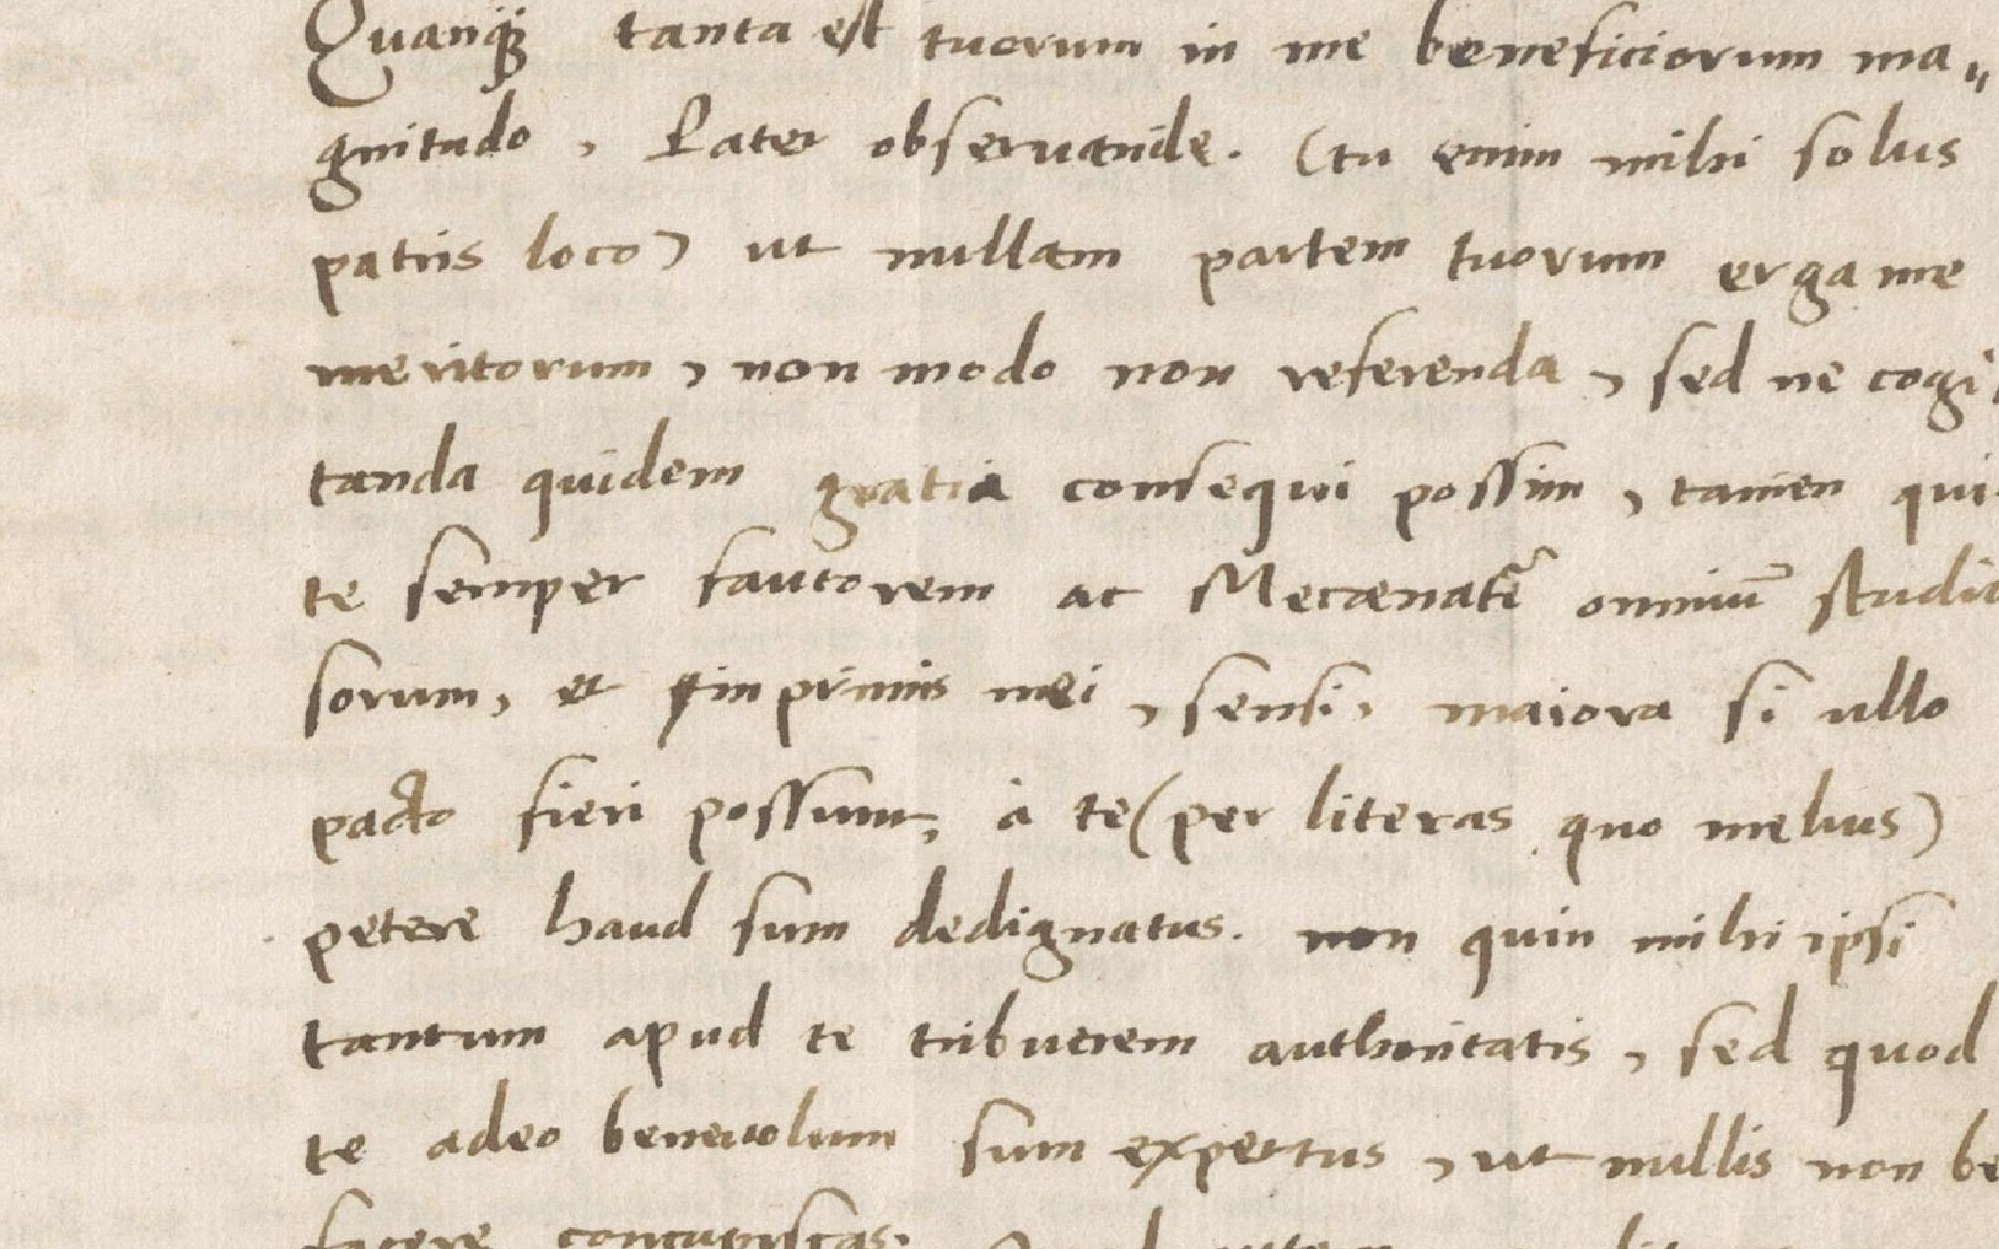
\includegraphics[width=0.47\textwidth]{images/pdf_optimized/ch4_bullinger_10333_0001_crop.jpg}}
  \hfill
  \subfigure[Children.]{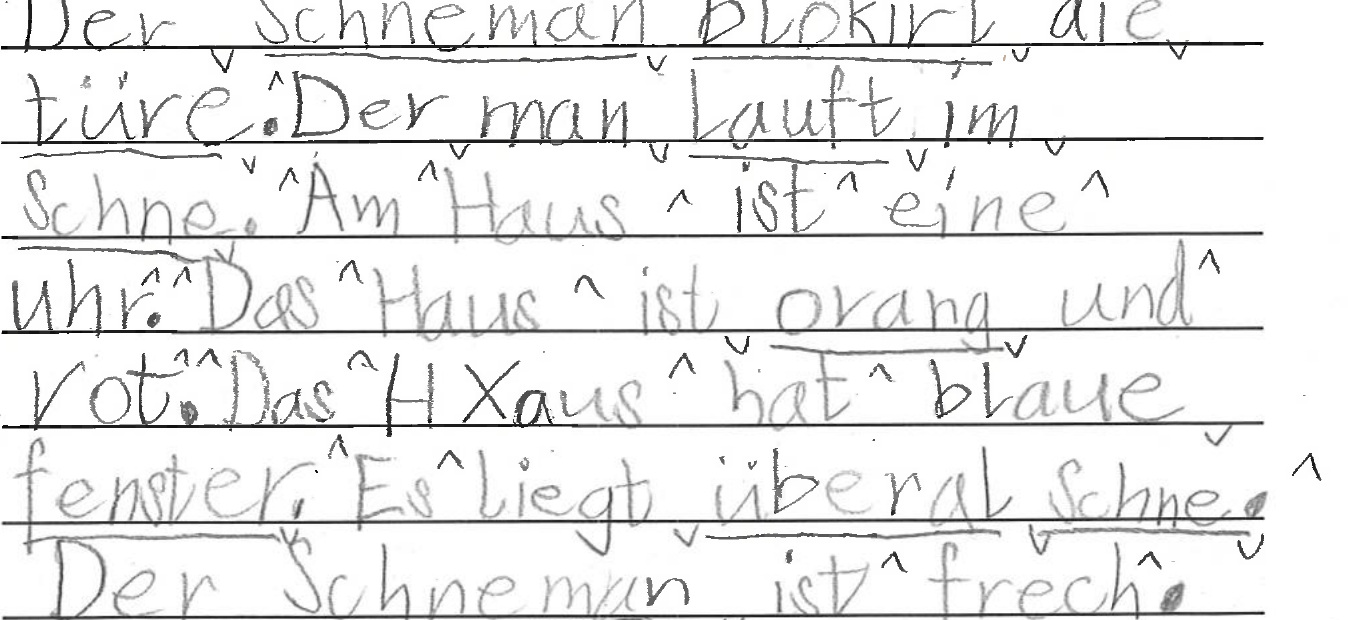
\includegraphics[width=0.47\textwidth]{images/pdf_optimized/ch4_children_1A_17_2_crop.jpg}}

  \vspace{0.6em}

  \subfigure[IAM.]{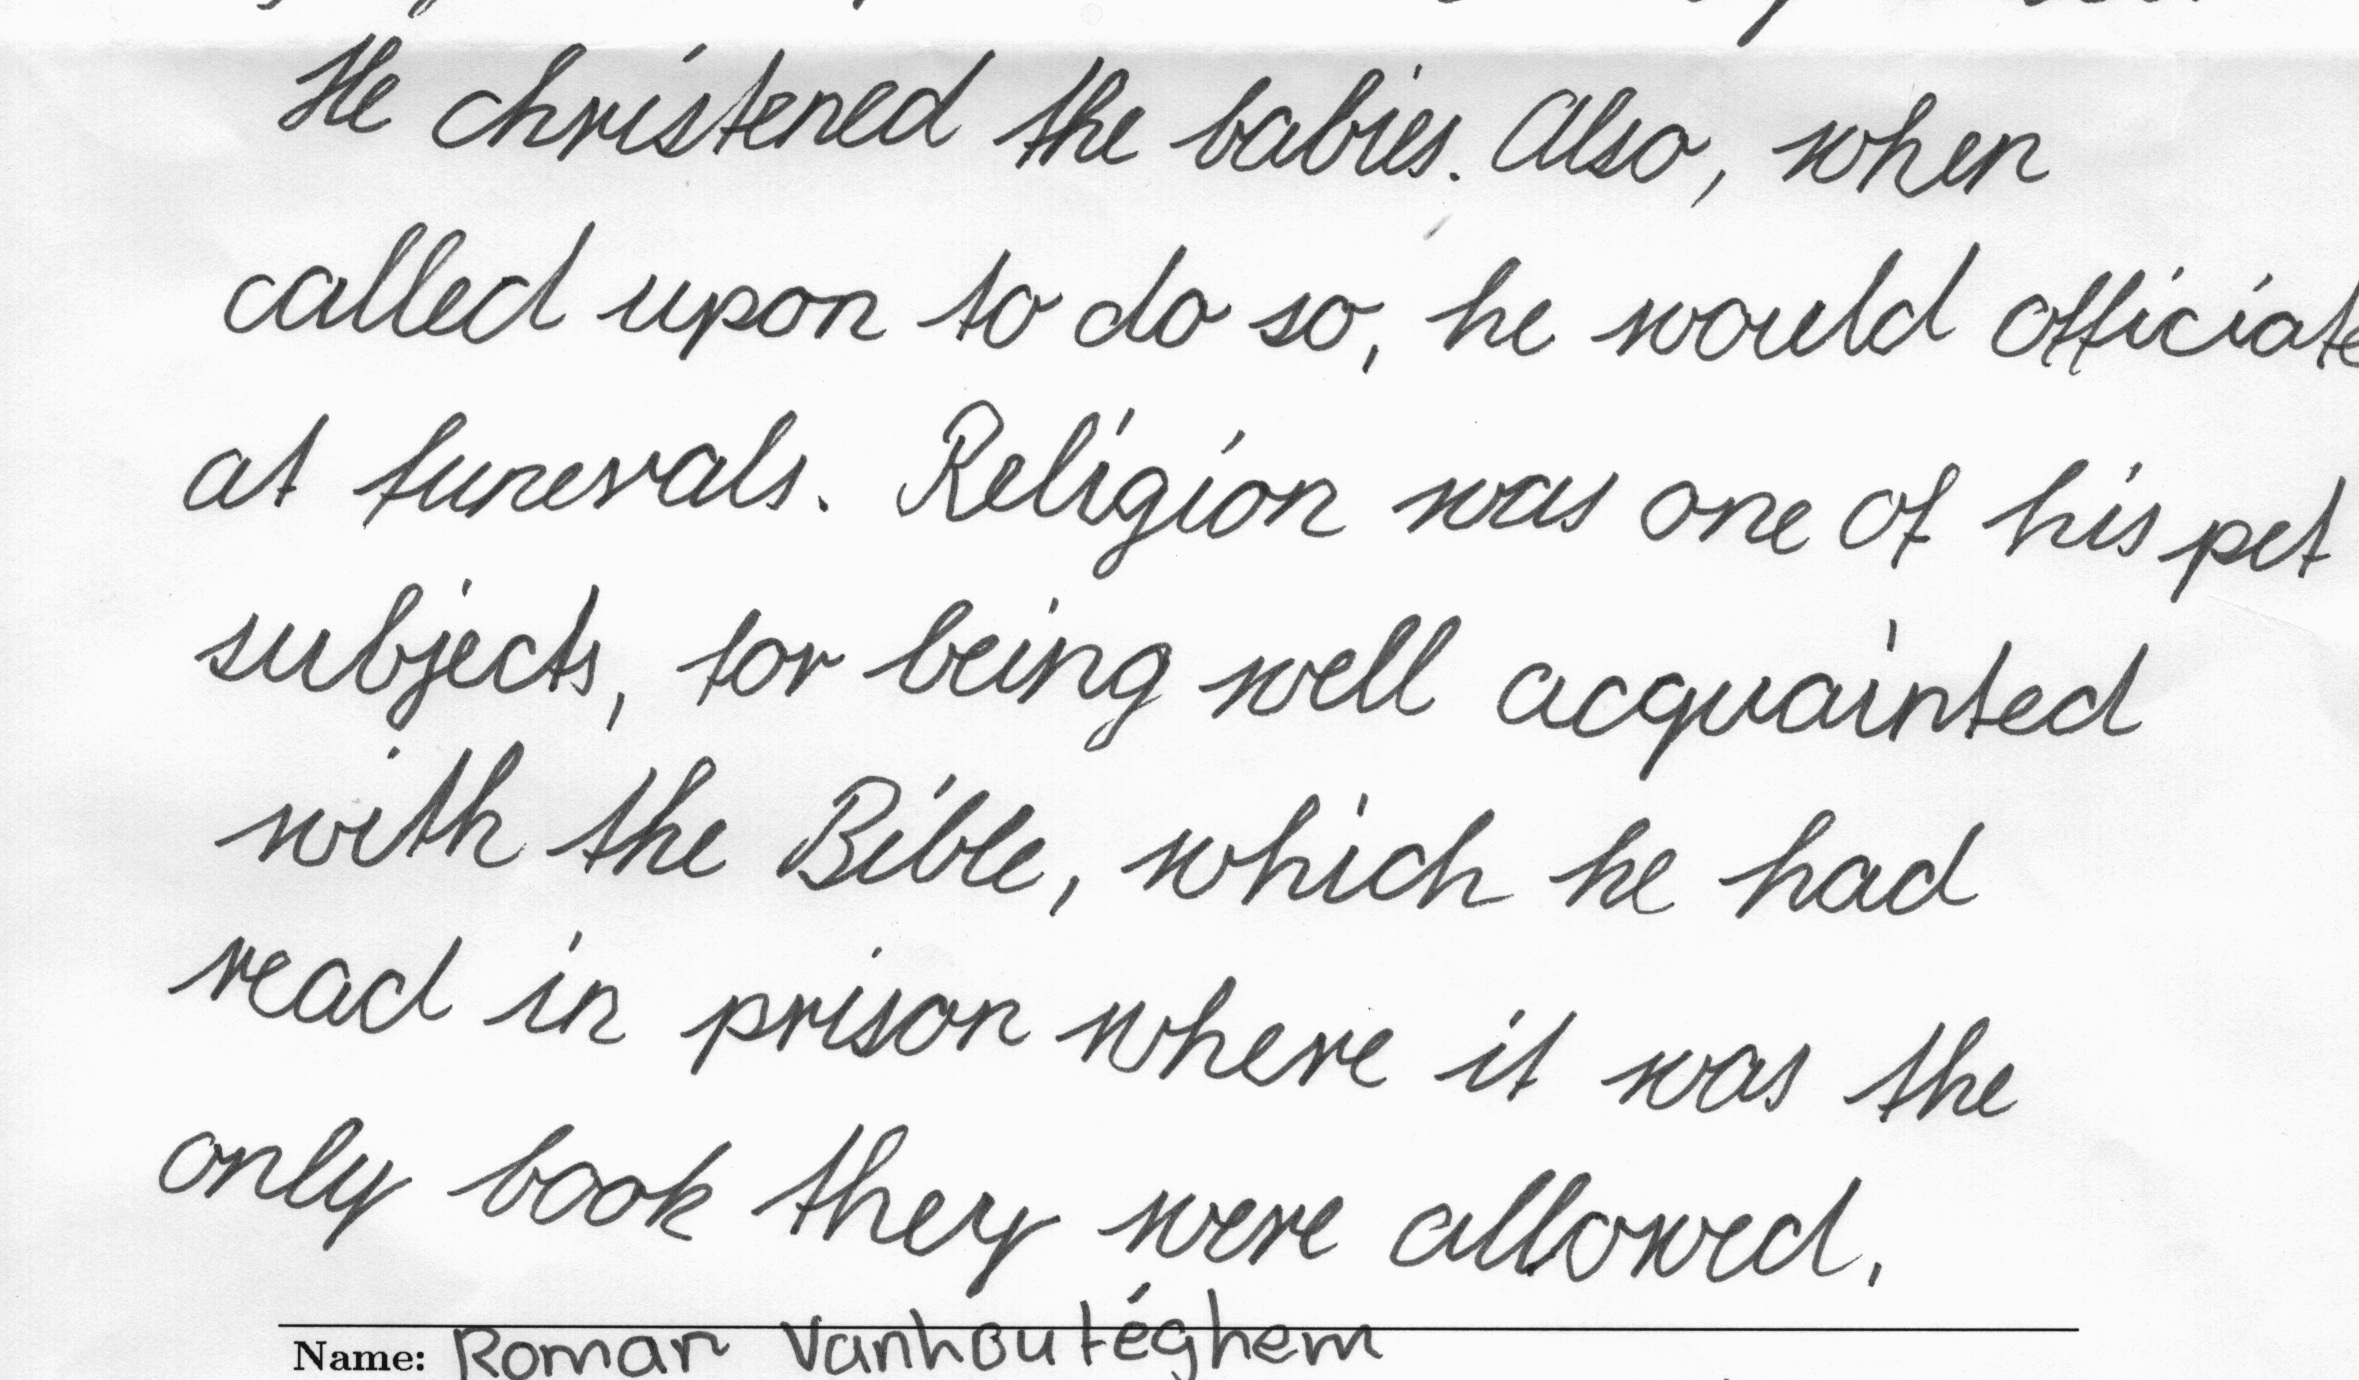
\includegraphics[width=0.47\textwidth]{images/pdf_optimized/ch4_iam_rep20_g03-043_crop.jpg}}
  \hfill
  \subfigure[Washington.]{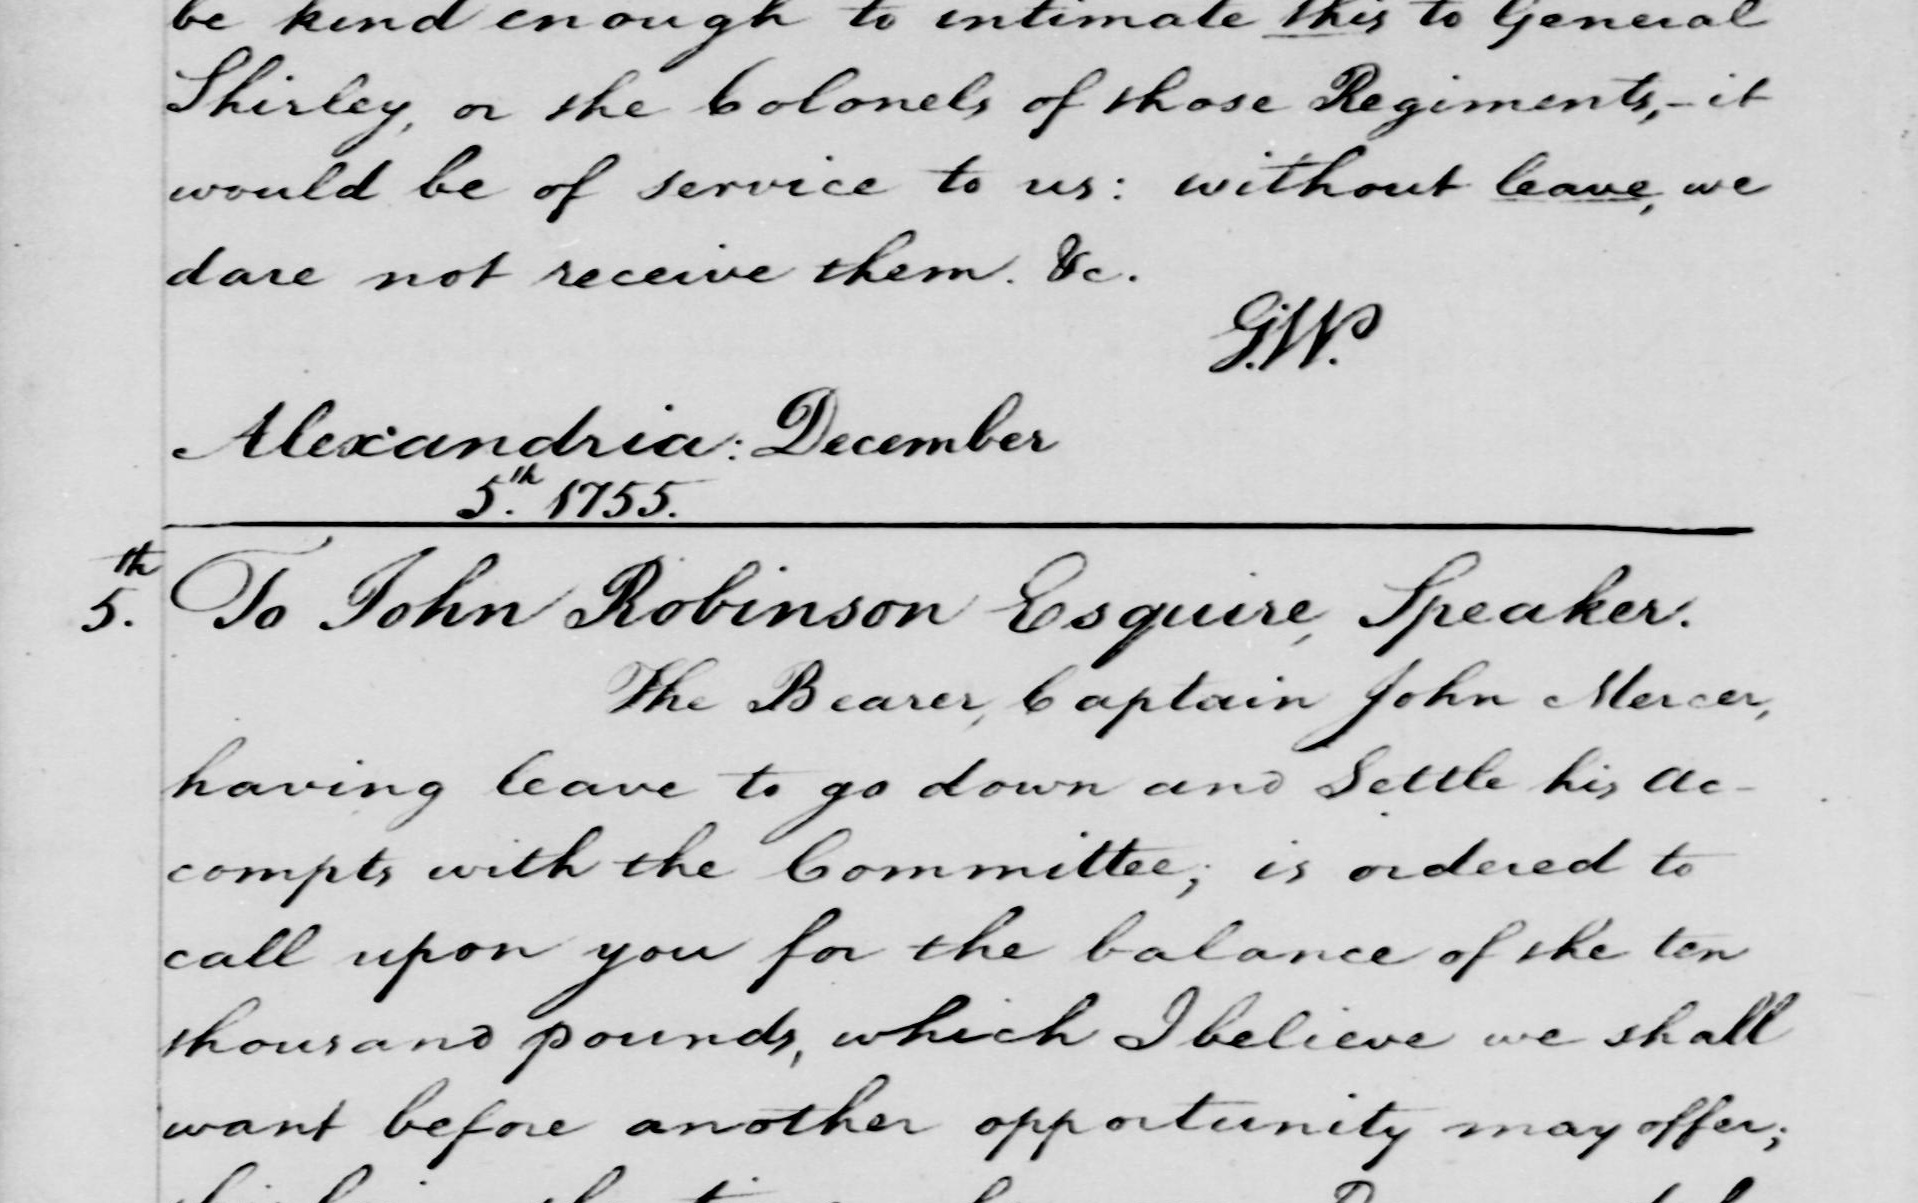
\includegraphics[width=0.47\textwidth]{images/pdf_optimized/ch4_washington_304_crop.jpg}}
  \caption{Cropped line-region examples from the four handwritten evaluation datasets. The panels emphasize visual heterogeneity across dense historical writing, ruled child handwriting, regular IAM forms, and degraded or structured Washington pages.}
  \label{fig:data_handwritten_page_examples}
\end{figure}

\subsection{Bullinger Handwritten and Print}
\label{sec:data_bullinger}

Bullinger Handwritten is a historical correspondence subset consisting of 59 letter-level samples. The reported count therefore refers to letter/sample IDs rather than single pages: Together, the samples span 100 page images and 2{,}535 ground-truth lines. For this thesis, the evaluation set combines two author-provided parts: Subset~1 contributes 20 letters, 50 pages, and 902 lines, while Subset~2 contributes 39 letters, 50 pages, and 1{,}633 lines. This composition matters because Bullinger contributes dense correspondence layouts, multilingual and premodern writing practices, and manuscript-specific line-boundary ambiguity \thesiscite{peer2025ctcBullingerAlignment,nikolaidou2022historicalDatasetSurvey}.

The broader Bullinger dataset is linguistically diverse, primarily Latin and premodern German, with passages in Greek, Italian, French, and Hebrew \thesiscite{peer2025ctcBullingerAlignment}. In the evaluation staging, PAGE/XML annotations provide the line order and line crops, and the stored structured line metadata matches the ground-truth line count on all 59 handwritten samples. This means that the staged data contains PAGE/XML-derived line order and known line counts; it is not evidence for blind page-side line detection.

\paragraph{Bullinger version note.}
The Bullinger subset used in this thesis is an author-provided version shared by Marco Peer. A provenance note from the author correspondence records that this subset version is acceptable for thesis use and that reevaluating all Bullinger runs consistently on that same subset keeps the thesis-side comparisons fair.\footnote{Provenance information, not a bibliographic source: Marco Peer, email communication with the author, 22 April 2026. The note also records that the final paper subset was not published in exactly the same form, that letter swaps after contamination checks introduced version drift relative to the paper description, and that the final official Subset~2 inventory may contain 1483 rather than 1486 lines.} Chapter~\ref{cha:experimentation} therefore separates the fairness of the internal thesis comparisons from the specific question of direct comparability in the Bullinger published-baseline comparison. The published Bullinger study remains cited as the external source for the dataset and reported baseline context \thesiscite{peer2025ctcBullingerAlignment}.

Bullinger Print is the printed Bullinger counterpart used as supporting context. It contains 10 printed Bullinger letter samples, each represented by one page image, for a total of 271 ground-truth lines. It preserves part of the historical-document setting while replacing handwriting with printed typography, making it useful for inspecting how the newline-only task behaves under a different visual modality. In the evaluation staging for this thesis, it provides page images, fixed transcriptions, line-broken ground truth, and OCR text; structured line metadata and line-image crops are not part of this printed staging.

For Bullinger, the retained printed-context artifacts also include a same-ID handwritten support slice for M1--M3. This makes a restricted print--handwriting comparison possible on the shared support IDs, but it does not change the main 59-sample Bullinger Handwritten denominator used for the primary handwritten evaluation.

\subsection{Children Handwritten}
\label{sec:data_children}

Children Handwritten contains unpublished AIBEX-provided handwritten material. The reported count means 63 evaluated handwritten samples, each represented by one page image, for a total of 394 ground-truth lines. It adds modern child handwriting to a portfolio otherwise dominated by historical manuscript and public benchmark material. The relevant variation is writer age, school-writing context, German language material, and child-specific spelling and orthographic variation.

The evaluation staging preserves dataset-provided presegmented line-image folders from the controlled source export and standardizes their order. The resulting line-image inventory contains one line crop per ground-truth line, and the stored structured line metadata matches the ground-truth line count on all 63 samples. No public per-sample language metadata is available for this restricted export, so the chapter describes language and provenance only at aggregate level.

\paragraph{Children Handwritten governance note.}
Children Handwritten is restricted AIBEX-provided evaluation material. The thesis reports aggregate evaluation results and includes only supervisor- or dataset-owner-approved short qualitative excerpts and selected illustrative cropped images needed for analysis. The underlying dataset, full page images, full per-sample transcriptions, source manifests, and controlled export files are not redistributed with this thesis. Any external reuse or redistribution requires approval from the dataset owner or supervisor.

Children Handwritten remains reproducible only for researchers who have access to the controlled AIBEX source export. The thesis can disclose the dataset-level denominators, build logic, and evaluation code, but not the underlying images, per-sample transcriptions, or the controlled source manifest. External reruns therefore require the same restricted source export and owner approval; without that access, the thesis supports protocol transparency but not fully public package-level replication.

\subsection{IAM Handwritten and Print}
\label{sec:data_iam}

IAM Handwritten denotes the fixed 20-form representative subset used in the thesis, not the full IAM handwriting collection. The reported count therefore means 20 IAM forms, each treated as one page/form sample, for a total of 180 ground-truth lines. The subset is materialized as an explicit form list rather than generated by random sampling at evaluation time. Within that fixed subset, the 20 forms span 17 writer prefixes and cover a 4--12 lines-per-form range, compared with 4--13 in the full RWTH test split. The IAM database and the RWTH split provide the public benchmark anchor for modern English handwriting \thesiscite{marti2002iam,zimmermann2002iamSeg,openslr56iam}.

IAM Handwritten contributes controlled modern handwriting with public provenance and official IAM form and line images. The thesis staging uses the official IAM line indices within each form; the stored structured line metadata over official IAM line images matches the ground-truth line count on all 20 forms. This makes IAM useful as a comparatively regular, public, modern handwriting anchor rather than as another historical collection.

IAM Print contains the machine-printed IAM text regions staged as printed form/page samples. The reported count means 30 forms/pages in the staged dataset, totaling 161 ground-truth print lines. It is printed, not handwritten, and it is not the same denominator as the 20-form handwritten representative subset. As supporting printed context, it adds a clean, modern counterpart to the handwritten IAM material while preserving the same general form/page source family. Its modality contribution lies in regular typography and short printed line blocks. Like Bullinger Print, it provides page images, fixed transcriptions, line-broken ground truth, and OCR text; structured line metadata and line-image crops are not part of this printed staging.

For IAM, the retained printed-context artifacts include a paired 30-form \texttt{a01-*} handwritten support slice for M1--M3. This paired slice supports a direct diagnostic print--handwriting comparison in Chapter~\ref{cha:experimentation}, but it is separate from the fixed representative-20 IAM Handwritten denominator used in the main evaluation.

\subsection{Washington Handwritten}
\label{sec:data_washington}

Washington Handwritten contains a 20-page historical handwritten evaluation set. The reported count means 20 page samples, each represented by one page image, for a total of 656 ground-truth lines. It contributes eighteenth-century English manuscript writing with a different historical source, page style, and degradation profile from Bullinger \thesiscite{lavrenko2004holisticWordRecognition}. In the portfolio, Washington therefore adds historical English writing, relatively dense page-level line structure, and a separate manuscript tradition.

Washington Handwritten uses a reviewed crop layer derived from a raw Kraken segmentation workspace. The evaluation version preserves the raw segmentation manifests separately and then rewrites the final staged crop inventory through reviewed merge, drop, split, insert, and bounding-box edits until the staged crop count matches the ground-truth line count on every evaluated page. The data boundary is therefore explicit: The staged version contains a curated one-crop-per-line inventory for alignment, not a blind page-side line-detection benchmark.

\section{Shared Artifacts and Preprocessing}
\label{sec:data_representation}
\label{sec:data_handwritten_artifact_availability}
\label{sec:data_ocr_provenance}

The six staged datasets share the same core sample schema: Line-broken ground truth, fixed transcription without line breaks, page images, and OCR/HTR text. The primary handwritten datasets additionally have structured line metadata in \texttt{ocr\_lines} records and line-image crops for every evaluated sample. The printed-context datasets do not include structured line metadata or line-image crop inventories in the staged datasets.

All evaluation datasets follow a common artifact representation per sample ID:
\begin{itemize}
  \item Ground truth text with line breaks,
  \item Fixed transcription without line breaks,
  \item Page image sequence,
  \item \OCRHTR text with line breaks,
  \item Ordered structured line metadata and line-image crops for the primary handwritten datasets.
\end{itemize}
This harmonization keeps the newline insertion target constant while allowing the later chapters to distinguish which evidence is available for each dataset. Table~\ref{tab:data_artifact_semantics} summarizes how each artifact maps to its task role.

Let sample $s$ be represented by
\[
(g_s, x_s, v_s, o_s, L_s),
\]
where $g_s$ denotes line-broken ground truth, $x_s$ the fixed transcription without line breaks, $v_s$ the ordered page-image sequence, $o_s$ the \OCRHTR output used as structural hint text, and $L_s$ the ordered line-image crop sequence when available or derivable. Relative to \autoref{sec:theory_problem_definition}, $x_s$ is the fixed character stream and only newline boundaries are predicted; $g_s$ is used exclusively for evaluation, while $o_s$ and $L_s$ serve as auxiliary structural evidence.

\begin{table}[H]
  \centering
  \caption{Artifact semantics per sample.}
  \label{tab:data_artifact_semantics}
  \begin{tabular}{@{}p{2.2cm}p{6.25cm}p{4.75cm}@{}}
    \toprule
    \textbf{Artifact} & \textbf{Semantics} & \textbf{Task role} \\
    \midrule
    $g_s$ & line-broken ground truth text for metric computation only & evaluation only \\
    $x_s$ & fixed transcription without line breaks & fixed character stream for newline insertion \\
    $v_s$ & ordered page images, single-page or multi-page depending on sample & page-level visual evidence \\
    $o_s$ & \OCRHTR text with line breaks as noisy structural hint & auxiliary textual line-structure evidence \\
    $L_s$ & ordered line-image crops from segmentation or dataset-provided line folders & line-level visual evidence where staged \\
    \bottomrule
  \end{tabular}
\end{table}

Table~\ref{tab:data_handwritten_artifact_availability} records the provenance of the handwritten line-level evidence. All four handwritten datasets provide complete sample-level coverage for page images, fixed transcriptions without line breaks, line-broken ground truth, \OCRHTR text, structured \texttt{ocr\_lines} JavaScript Object Notation (JSON), and line-image crops. The asymmetry is not whether line-level evidence exists, but how that evidence is produced and how line order and expected line count are fixed.

\begin{table}[H]
  \centering
  \caption{Line-level evidence provenance on the four handwritten evaluation datasets. Page images, fixed transcriptions, line-broken ground truth, \OCRHTR text, structured \OCRLinesPath{} metadata, and line-image crops are available for all evaluated handwritten samples; the table highlights the provenance dimensions that differ across datasets and constrain leakage, known-count assumptions, and reproducibility claims.}
  \label{tab:data_handwritten_artifact_availability}
  \footnotesize
  \renewcommand{\arraystretch}{1.08}
  \begin{tabularx}{\linewidth}{@{}>{\raggedright\arraybackslash}p{0.15\linewidth}>{\raggedright\arraybackslash}Y>{\raggedright\arraybackslash}Y>{\raggedright\arraybackslash}Y>{\raggedright\arraybackslash}Y@{}}
    \toprule
    \textbf{Dataset} & \textbf{Line-crop provenance} & \textbf{OCR-line text provenance} & \textbf{Source of line order} & \textbf{Expected line count source} \\
    \midrule
    Bullinger Handwritten (\(n=59\) letter samples) & PAGE/XML-derived line crops materialized from the author-provided Bullinger export & PyLaia OCR over PAGE/XML-derived line images & PAGE reading order from XML & stored \texttt{ocr\_lines} cardinality over PAGE/XML-derived lines; equals ground truth on 59/59 samples \\
    Children Handwritten (\(n=63\) samples) & dataset-provided presegmented line-image folders copied from the controlled source export & PyLaia OCR over dataset-provided line images & dataset crop order preserved by standardized line renaming in dataset build & stored \texttt{ocr\_lines} cardinality over dataset-provided line folders; equals ground truth on 63/63 samples \\
    IAM Handwritten (\(n=20\) forms) & official IAM line images staged from the RWTH test split & PyLaia OCR over official IAM line images & official IAM line indices within each form & stored \texttt{ocr\_lines} cardinality over official IAM line images; equals ground truth on 20/20 forms \\
    Washington Handwritten (\(n=20\) page samples) & curated Kraken crops from the reviewed Washington alignment workspace; staged inventory contains one crop per ground-truth line & OCR scaffold over the curated Kraken crop inventory & curated review order materialized into final \texttt{line\_index} order & stored \texttt{ocr\_lines} cardinality over curated one-crop-per-line staging; equals ground truth on 20/20 samples \\
    \bottomrule
  \end{tabularx}
\end{table}

The OCR/HTR hint artifact $o_s$ is generated by a unified pipeline that first segments page images into line crops and then recognizes each crop as text. At software level, the implementation supports Kraken segmentation \thesiscite{kiessling2025kraken}, TrOCR recognition presets \thesiscite{li2023trocr}, optional docTR segmentation \thesiscite{mindee2026doctr}, and passthrough reuse of already segmented line folders. Dataset-specific choices are summarized in Table~\ref{tab:data_handwritten_artifact_availability}; the printed-context datasets use printed-recognition OCR hints but not the handwritten structured line-crop layer.

For multi-page samples, recognized text is concatenated in page order with explicit page-level separation, preserving sample-level sequence semantics for downstream alignment. Cacheable line crops and optional metadata sidecars are used to make \OCRHTR generation repeatable across reruns and cluster jobs; the reusable artifact chain is summarized in Table~\ref{tab:method_reproducibility_artifacts}.

\section{Data Quality and Validity Considerations}
\label{sec:data_threats}

Dataset heterogeneity is both a strength and a risk: Mixing historical and modern material improves coverage but increases variance in writing style, page condition, and language conventions. Domain shift under OCR noise is known to alter downstream textual behavior, so conclusions should be interpreted per dataset first and only then aggregated \thesiscite{nikolaidou2022historicalDatasetSurvey,marz2021dataCentricDomainAdaptation}.

At line level, annotation and boundary ambiguity remain inherent in historical documents because multiple nearby separators can be plausible under touching strokes, skew, bleed-through, or marginal additions. Therefore, absolute score differences should be interpreted together with qualitative evidence and complementary metrics rather than as purely geometric truth/falsehood decisions \thesiscite{likformansulem2006textLineSurvey,gruning2018readbad}.

A known-count assumption is a construct-validity boundary for the structured handwritten rows discussed in later chapters. The stored \texttt{ocr\_lines} payload provides the expected number of output lines, and that cardinality matches the ground-truth line count on every evaluated handwritten sample. This is especially important for Washington Handwritten, where the committed crop layer is curated until the staged inventory contains one crop per ground-truth line. These settings are still informative for newline placement under aligned line evidence, but they should not be interpreted as blind end-to-end page segmentation or page-side line-count prediction.

OCR/HTR enters the evaluation as auxiliary structural evidence rather than as the target to be scored. Whenever a regime relies on OCR/HTR text or structured OCR-line metadata, recognition errors can propagate into boundary suggestions. This creates a dependency between OCR quality and alignment outcomes that does not exist in purely image-guided settings, and it motivates keeping OCR-conditioned evidence analytically separate from image-side evidence in later reporting \thesiscite{li2023trocr,liu2024ocrbench}.

Where ordered line-image crops are used, line-level evidence quality becomes the critical dependency. Segmentation mistakes, crop ordering errors, or incomplete line folders can degrade alignment even when the downstream model or recognizer is otherwise strong. This point applies to the primary handwritten staging, because the printed-context datasets do not include line-image inventories \thesiscite{likformansulem2006textLineSurvey,graves2006ctc}.

The printed-context datasets broaden the modality inventory while remaining analytically secondary. Bullinger Print and IAM Print are useful for checking the newline-only task outside handwriting, but the experimentation chapter treats them as an additional printed context layer rather than as a second full evaluation portfolio. They should not be merged silently into the primary handwritten evidence base.

NNTP is evaluated with the same downstream metric family, but it filters labels to the active PyLaia \texttt{syms.txt} alphabet before alignment. This does not remove its role as a deterministic forced-alignment baseline, but it matters whenever character-level comparability with M1--M5 is interpreted. For data-level purposes, the key point is that NNTP is most directly comparable on the shared line-metric surface; Chapter~\ref{cha:experimentation} carries the same-sample and contextual result split.

The sample distribution is imbalanced across datasets: The handwritten denominators range from 20 to 63 samples, and the printed denominators are 10 and 30 samples. Macro-level interpretation should therefore avoid over-weighting larger or cleaner subsets in narrative conclusions. The experimentation chapter reports per-dataset results before drawing broader comparative interpretations.

\label{sec:data_summary}
This chapter defines the primary handwritten evaluation datasets, the additional printed-context datasets, the shared artifact schema, and the provenance differences that matter for interpreting later method and result claims. These definitions anchor the method instantiations in \autoref{cha:method} and the quantitative reporting protocol in \autoref{cha:experimentation}, especially the distinction between complete artifact coverage and heterogeneous line-level evidence provenance.

% Chapter 5 describes the implemented methods and their design rationale.
% Content: newline-only evaluation target, method definitions for Methods 1--5 and NNTP,
% OCR/HTR generation pipeline, and implementation safeguards.

\chapter{Methods}
\label{cha:method}

\section{Scope and Contribution Framing}
\label{sec:method_scope}

This chapter provides the methodological overview for the thesis task. The starting point is the same throughout: Historical transcriptions may already provide the character sequence, but scholarly reuse still requires recovering the line structure. The newline-only formulation isolates that problem by holding the non-newline character sequence fixed and asking where line boundaries should be inserted. The methodological description therefore specifies how the formal task from \autoref{sec:theory_problem_definition} is instantiated as evaluated alignment regimes in the sense defined in Chapter~\ref{cha:introduction}: Which evidence each configuration sees, which output constraint it is asked to satisfy, which evaluated LLM/VLM configurations instantiate the benchmark, and which recovery steps belong to the scored setup. Exact template identifiers, prompt-template/source mappings, and run-configuration details are deferred to Appendix~\ref{cha:appendix_audit} and the companion implementation repository.\footnote{Implementation provenance: \url{https://github.com/dennis-berger/llm-line-alignment}}

At the method level, the contribution has three parts: A shared newline-only transcription-alignment target, a set of LLM/VLM-based methods whose evaluated configurations vary along two design dimensions, and the deterministic baseline (NNTP) evaluated with the same downstream metric family. The five LLM/VLM-based methods are referred to as Method 1 to Method 5 (M1--M5). Their configurations are organized over two design questions: Which input evidence can support boundary placement, and how far the system should constrain, validate, repair, or project the model output before scoring \thesiscite{geng2023grammar}. The deterministic baseline is included because Connectionist Temporal Classification (CTC) transcription alignment is a close forced-alignment analogue of the thesis task: It preserves a supplied transcription and searches for line-boundary placements using recognizer-derived evidence rather than prompting a model to produce a fresh transcription \thesiscite{fischer2011icdarInaccurateAlignment,hassner2013ocrFreeAlignment,peer2025ctcBullingerAlignment}. This framing makes it possible to compare LLM/VLM-based configurations and deterministic alignment under one task scope while still keeping their setup differences explicit.

\section{Shared Transcription-Alignment Target}
\label{sec:method_common_contract}

For M1--M5, the prediction target is always the same: Recover line boundaries in a supplied transcription without changing the underlying character sequence. The fixed transcription is therefore the only admissible character source, and the LLM/VLM-based methods are designed to place newline boundaries rather than to generate new lexical content. This is the methodological move that separates line-structure recovery from recognition quality.

The evaluation target is shared, but the enforcement strength is method-dependent and part of the evaluated configuration. M1--M3 rely on prompt instructions alone and score the raw returned text directly. M4 and M5 instead ask for strict JSON of the form \texttt{\{"lines": [...]\}}, validate the returned array after generation, and, depending on the configuration, enter bounded repair, recovery, or fallback paths when the output is malformed or structurally implausible. In relation to prior work on constrained structure recovery and alignment \thesiscite{geng2023grammar,fischer2011icdarInaccurateAlignment}, the reported thesis mechanism is specifically parser-side validation plus repair rather than provider-side grammar-constrained decoding; the implemented control path is summarized in Algorithm~\ref{alg:method_structured_post_correction} and expanded in \autoref{sec:appendix_structured_pseudocode}.

For M4 and M5, exact-character preservation is achieved through boundary projection rather than by trusting copied model text. The implementation keeps the predicted line-boundary plan, maps those boundaries from the hinted text back onto the untouched supplied transcription, and stores the projected boundary plan for evaluation. Repair, method-specific recovery, fallback, and projection are therefore part of the evaluated configuration for M4 and M5 rather than a post-hoc clean-up layer outside scoring; this implementation-specific output-control path is recorded in Table~\ref{tab:method_prompt_contract} and \autoref{sec:appendix_structured_audit}.

All LLM/VLM-based configurations are evaluated by the shared metric stack from \autoref{sec:experimentation_line_alignment_metrics}. NNTP is evaluated with the same downstream metrics, but its preparation stage normalizes and filters labels to the active PyLaia symbol inventory before alignment. The shared evaluation is therefore strong at the metric level, especially for line-boundary outcomes, yet not perfectly identical at the character-inventory level.

The method scope is handwritten-first. M1--M5 form the main handwritten evaluation on the four handwritten datasets, while Bullinger Print and IAM Print are reported as secondary printed context. The focused print evaluation covers M1--M3 rather than the line-image and structured-output configurations, so it should not be read as evidence for the full M1--M5 method set.

\paragraph{Prompt design principles.}
\label{sec:method_prompt_principles}

Table~\ref{tab:method_prompt_contract} summarizes the thesis-level prompt requirements shared by the LLM/VLM-based method set. It describes the scientific intent of the prompts rather than reproducing their full wording. Exact implementation identifiers, prompt-template/source mappings, and run-configuration details are listed in \autoref{sec:appendix_prompt_templates}.

\begin{table}[H]
  \centering
  \caption{Compact schematic prompt requirements for the LLM/VLM-based method set.}
  \label{tab:method_prompt_contract}
  \small
  \renewcommand{\arraystretch}{1.08}
  \begin{tabularx}{\linewidth}{@{}p{0.25\linewidth}Y@{}}
    \toprule
    \textbf{Aspect} & \textbf{Requirement} \\
    \midrule
    Character source & The supplied transcription is the only admissible source of characters. \\
    Allowed edit & Only newline boundaries may be inserted; the character sequence itself must remain fixed. \\
    Normalization & No spelling correction, modernization, normalization, or semantic rewriting is allowed. \\
    OCR/HTR evidence & OCR/HTR is used only as structural evidence about likely boundaries and reading order, never as replacement text. \\
    Structured output (M4/M5) & The response must be strict JSON with exactly \(N\) lines, where \(N\) is the expected line count supplied by the evaluated configuration. \\
    Failure handling (M4/M5) & If the strict JSON requirement fails, the configuration may attempt one repair pass, method-specific recovery from model lines, or deterministic fallback before final projection to the supplied transcription. \\
    \bottomrule
  \end{tabularx}
\end{table}

The requirements in Table~\ref{tab:method_prompt_contract} also clarify the main asymmetry inside M1--M5. M1--M3 depend entirely on whether the initial prompt is followed faithfully, whereas M4 and M5 score a controlled boundary plan after validation and, when needed, recovery. This distinction belongs to the method definition itself: Later comparisons inherit a shared target, but not identical output-control strength.

\section{Method Set Overview}
\label{sec:method_overview}

With the newline-only constraint fixed, the method set is organised by two design axes rather than by a single incremental ladder. The first axis is \emph{input evidence}: Page images, OCR/HTR text, ordered OCR-line metadata, ordered line crops, and recognizer observations each expose different boundary cues. The second axis is \emph{output control}: Raw returned text, structured JSON validation, repair or fallback, projection to the supplied transcription, and deterministic forced alignment make different commitments about how a candidate boundary plan becomes the scored object. The overview tables and figures therefore introduce a design space before the individual method descriptions supply operational detail.

Intuitively, M1--M3 ask how much boundary evidence remains useful under weak output control, where the raw returned text is scored directly. M4--M5 test structured output control together with richer line-level evidence, so the evaluated object is a projected boundary plan selected from accepted, repaired, recovered, or fallback hints. NNTP then provides a deterministic forced-alignment anchor rather than another prompted generation configuration.

\begin{table}[t]
  \centering
  \caption{Method-set overview for the implemented configurations. M1--M5 share the newline-only target but vary along the evidence and output-control dimensions; NNTP is the deterministic baseline evaluated with the same downstream metric family but with PyLaia-filtered labels.}
  \label{tab:method_regime_comparison}
  \small
  \renewcommand{\arraystretch}{1.08}
  \setlength{\tabcolsep}{4pt}
  \begin{tabularx}{\linewidth}{@{}>{\raggedright\arraybackslash}p{0.18\linewidth}>{\raggedright\arraybackslash}p{0.11\linewidth}>{\raggedright\arraybackslash}p{0.23\linewidth}>{\raggedright\arraybackslash}p{0.20\linewidth}>{\raggedright\arraybackslash}X@{}}
    \toprule
    \textbf{Configuration family} & \textbf{Methods} & \textbf{Input evidence} & \textbf{Output control} & \textbf{Purpose in the thesis} \\
    \midrule
    Raw LLM/VLM output regimes & M1--M3 & Supplied transcription plus page images, \OCRHTR text, or both, depending on the concrete configuration & Prompt instructions only; raw returned text is scored directly & Tests how much boundary structure can be recovered by changing the evidence supplied to an otherwise raw-output configuration \\
    Structured LLM/VLM regimes & M4--M5 & Supplied transcription plus ordered OCR-line metadata or ordered line-image crops; the evaluated M5 configuration also supplies OCR/HTR line text and page-level context & Strict JSON, parser validation, one repair pass, method-specific fallback or recovery, and projection to the supplied transcription & Tests whether stronger output-control paths and line-level anchors reduce character drift and boundary ambiguity \\
    Deterministic baseline & NNTP & Fixed transcription, ordered line-image evidence, and recognizer-derived CTC observations & Deterministic forced alignment over labels filtered to the active PyLaia symbol inventory & Provides a non-prompt comparison for the same newline-boundary metric family while keeping the symbol-filtering caveat explicit \\
    \bottomrule
  \end{tabularx}
\end{table}

The key comparison axis in \autoref{tab:method_regime_comparison} combines which modality is present with how strongly structure is anchored and how strongly outputs are controlled afterward. M1--M3 isolate evidence choices inside a raw LLM/VLM output configuration; M4--M5 combine line-level evidence with structured response validation and projection; NNTP replaces generative prompting with deterministic forced alignment over recognizer observations. The table should therefore be read as an inventory of implemented configurations, not as a ladder in which a single factor changes at a time.

\begin{table}[H]
  \centering
  \caption{Compact method cards for the implemented regimes. The table keeps the main-text interpretation variables; \autoref{sec:appendix_method_comparability} expands them into the appendix comparability registry.}
  \label{tab:method_comparability_matrix}
  \scriptsize
  \renewcommand{\arraystretch}{1.06}
  \setlength{\tabcolsep}{2pt}
  \begin{tabularx}{\linewidth}{@{}>{\raggedright\arraybackslash}p{0.055\linewidth}*{7}{>{\raggedright\arraybackslash}X}@{}}
    \toprule
    \textbf{Method} & \textbf{Input evidence} & \textbf{Expected line-count source} & \textbf{Output type} & \textbf{Validation/repair} & \textbf{Projection/\allowbreak fallback} & \textbf{Scored object} & \textbf{Main caveat} \\
    \midrule
    M1 & page image(s) + fixed transcription & none; count emerges & line-broken text & prompt only & none & raw returned text & heuristic page chunking \\
    M2 & page image(s) + \OCRHTR{} hint + fixed transcription & none; count emerges & line-broken text & prompt only & none & raw returned text & OCR noise + chunking \\
    M3 & \OCRHTR{} hint + fixed transcription & none; count emerges & line-broken text & prompt only & none & raw returned text & no visual correction \\
    M4 & ordered OCR-line scaffold + expected \(N\) + fixed transcription & stored \texttt{ocr\_lines} count & JSON line list & parse; exact \(N\); one repair & project accepted or fallback plan & projected boundary plan & known count; OCR scaffold \\
    M5 & ordered line crops + \OCRHTR{} line text + page context + expected \(N\) + fixed transcription & stored \texttt{ocr\_lines} count & JSON line list & parse; exact \(N\); repair/checks & recovery or fallback; projection & projected boundary plan & heterogeneous crop provenance; image-packaging limits \\
    NNTP & line images + recognizer output + fixed transcription & staged line-image set & forced-alignment reconstruction & deterministic checks & not applicable & filtered reconstruction & PyLaia symbol-inventory filter \\
    \bottomrule
  \end{tabularx}
\par\vspace{0.35em}
  \parbox{0.98\linewidth}{\footnotesize\raggedright \textit{Note.} The caveat column is intentionally compact. Table~\ref{tab:method_line_evidence_sources} consolidates the known-count and crop-provenance caveats for M4/M5, while \autoref{sec:method_safeguards_limits} collects the cross-method interpretation limits, including backend image-packaging limits and NNTP's PyLaia-side symbol filtering.}
\end{table}

\paragraph{What is scored?}
M1--M3 score raw returned text: Copied-character changes, omissions, normalizations, or extra prose remain part of the prediction. M4 and M5 score projected boundary plans selected from accepted, repaired, recovered, or fallback hints. NNTP scores deterministic reconstruction after PyLaia-side filtering. This is the same scored-object distinction used by the Chapter~\ref{cha:experimentation} output-control analysis.

Figures~\ref{fig:method_regime_ladder} and~\ref{fig:method_pipeline_overview} split that overview into two readable views. The first marks the boundary between raw-output M1--M3 and structured M4/M5, while the second isolates the shared structured-control skeleton from stored ordered line metadata to evaluation. Dataset-specific crop provenance stays in Table~\ref{tab:method_line_evidence_sources}, while \autoref{sec:appendix_structured_audit} holds the fuller structured-control tables used later for traceability.

\begin{figure}[H]
  \centering
  \begin{tikzpicture}[
    x=1cm,
    y=1cm,
    font=\footnotesize,
    method/.style={rectangle, rounded corners=3pt, draw=black!70, thick, align=left, text width=11.1cm, minimum height=1.05cm, inner sep=5pt},
    raw/.style={method, fill=blue!8},
    structured/.style={method, fill=orange!15},
    baseline/.style={method, fill=green!12},
    tag/.style={rectangle, rounded corners=3pt, draw=black!70, thick, minimum width=1.0cm, minimum height=1.05cm, font=\bfseries},
    note/.style={rectangle, rounded corners=3pt, draw=orange!60!black, thick, fill=orange!8, align=left, text width=11.1cm, inner sep=5pt}
  ]
    \node[tag, fill=blue!18] (m1tag) at (0,0) {M1};
    \node[raw, anchor=west] (m1) at (0.85,0) {\textbf{Evidence:} Page images + fixed transcription \(x\)\\\textbf{Output path:} Raw model text evaluated directly};

    \node[tag, fill=blue!18] (m2tag) at (0,-1.55) {M2};
    \node[raw, anchor=west] (m2) at (0.85,-1.55) {\textbf{Evidence:} Page images + OCR/HTR + fixed transcription \(x\)\\\textbf{Output path:} Raw model text evaluated directly};

    \node[tag, fill=blue!18] (m3tag) at (0,-3.10) {M3};
    \node[raw, anchor=west] (m3) at (0.85,-3.10) {\textbf{Evidence:} OCR/HTR + fixed transcription \(x\)\\\textbf{Output path:} Raw model text evaluated directly};

    \draw[black!60, dashed, line width=0.9pt] (-0.45,-4.20) -- (12.20,-4.20);
    \node[fill=white, inner sep=2pt, font=\scriptsize\bfseries] at (5.90,-4.20) {Structured output and projection begin};
    \node[anchor=east, align=right, font=\scriptsize\bfseries] at (-0.55,-1.55) {Raw-output\\prompting};

    \node[note] (sharednote) at (6.40,-5.10) {\textbf{Shared M4/M5 count control:} Expected \(N\) is read from stored ordered line metadata and matches ground truth on the evaluated handwritten datasets.};
    \node[anchor=east, align=right, font=\scriptsize\bfseries] at (-0.55,-6.55) {Structured\\prompting};

    \node[tag, fill=orange!28] (m4tag) at (0,-6.55) {M4};
    \node[structured, anchor=west] (m4) at (0.85,-6.55) {\textbf{Evidence:} Ordered OCR-line scaffold + stored expected \(N\)\\\textbf{Output path:} Strict JSON, repair/fallback, projection};

    \node[tag, fill=orange!28] (m5tag) at (0,-8.10) {M5};
    \node[structured, anchor=west] (m5) at (0.85,-8.10) {\textbf{Evidence:} Ordered line crops + \OCRHTR{} line text + page context + stored expected \(N\)\\\textbf{Output path:} Strict JSON, repair/recovery/fallback, projection};

    \node[anchor=east, align=right, font=\scriptsize\bfseries] at (-0.55,-9.65) {Deterministic\\baseline};
    \node[tag, fill=green!24] (nntptag) at (0,-9.65) {NNTP};
    \node[baseline, anchor=west] (nntp) at (0.85,-9.65) {\textbf{Evidence:} Staged line images + recognizer observations + fixed transcription \(x\)\\\textbf{Output path:} Deterministic forced alignment; labels filtered to active PyLaia inventory};
  \end{tikzpicture}
  \caption{Evidence and output-control overview for the implemented M1--M5 configurations. The dashed divider marks the shift from raw-output prompting (M1--M3) to structured prompting with projection (M4--M5).}
  \label{fig:method_regime_ladder}
\end{figure}

\begin{figure}[H]
  \centering
  \begin{tikzpicture}[
    node distance=0.48cm,
    font=\footnotesize,
    >={Latex[length=2mm]},
    stage/.style={rectangle, rounded corners=3pt, draw=black!70, thick, align=center, text width=10.3cm, minimum height=0.95cm, inner sep=5pt},
    input/.style={stage, fill=gray!10},
    control/.style={stage, fill=orange!15},
    eval/.style={stage, fill=blue!8},
    flow/.style={->, thick}
  ]
    \node[input] (ocrjson) {stored ordered line metadata\\shared structured payload for M4/M5; M4 uses ordered OCR-line hints and evaluated M5 resolves ordered line crops plus \OCRHTR{} line text and page context};
    \node[input, below=of ocrjson] (count) {expected \(N\) read from stored metadata\\matches ground truth on the evaluated handwritten datasets};
    \node[control, below=of count] (strict) {strict JSON response\\\texttt{\{"lines": ["...", "..."]\}}};
    \node[control, below=of strict] (repair) {one repair prompt if the JSON is malformed or has the wrong line count};
    \node[control, below=of repair] (fallback) {recovery or deterministic fallback after the strict path fails\\(M5 may reconcile loose response lines; M4 falls back deterministically)};
    \node[control, below=of fallback] (projection) {projection of the selected boundary plan back onto the untouched transcription \(x\)};
    \node[eval, below=of projection] (evaluation) {evaluation\\line accuracy, exact-line precision/recall/F1, raw/normalized CER/WER};

    \draw[flow] (ocrjson) -- (count);
    \draw[flow] (count) -- (strict);
    \draw[flow] (strict) -- (repair);
    \draw[flow] (repair) -- (fallback);
    \draw[flow] (fallback) -- (projection);
    \draw[flow] (projection) -- (evaluation);
  \end{tikzpicture}
  \caption{Structured-output control skeleton for M4 and M5. Raw-output methods M1--M3 are excluded because they do not pass through known-count staging, JSON validation, repair/fallback, and projection; M5 additionally includes recovery and page-wise subdivision for long inputs.}
  \label{fig:method_pipeline_overview}
\end{figure}

\FloatBarrier

\section{Benchmarked LLM/VLM Model Families and Capabilities}
\label{sec:method_benchmarked_models}

The LLM/VLM part of the benchmark uses contemporary general-purpose multimodal model families rather than task-specific handwriting recognizers or dedicated transcript-alignment models. The relevant capability is not only visual recognition. For newline-only alignment, a model must be able to receive document-image evidence and textual context, follow instructions about a fixed transcription, and return either line-broken text or a structured representation that can later be validated and projected back to the supplied transcription. This section records the model families and capabilities needed to interpret the benchmark \thesiscite{openai2026gpt54,openai2026models,google2026geminiModels,google2026gemini25Models,bai2025qwen3vl,mistral2026models,mistral2026vision}.

\paragraph{OpenAI GPT configurations.}
The OpenAI configurations are hosted multimodal LLM/VLM systems used through an API backend. In the thesis artifacts they are represented by the display names GPT-5.4-0305 and GPT-5.2. The important capability for this work is that these configurations support text interaction together with image input, so they can be prompted with a fixed transcription plus page or line-image evidence. GPT-5.4-0305 is treated as the main OpenAI configuration in the benchmark, while GPT-5.2 is retained as an earlier OpenAI configuration for historical and diagnostic context. The display names used in the thesis refer to the archived provider identifiers recorded in Appendix Table~\ref{tab:app_model_provider_aliases}, not to later model versions or later provider behavior \thesiscite{openai2026gpt54,openai2026models}.

\paragraph{Google Gemini configurations.}
The Gemini configurations represent Google's hosted multimodal model family. They are included because the task requires a general-purpose model that can combine visual document evidence with textual instructions and \OCRHTR{}-derived context. In this thesis, Gemini rows are used as additional provider evidence rather than as an architectural study of the Gemini family. The exact Gemini display names, provider identifiers, and retained experiment rows are documented in Appendix Table~\ref{tab:app_model_provider_aliases} \thesiscite{google2026geminiModels,google2026gemini25Models}.

\paragraph{Qwen3-VL configurations.}
Qwen3-VL represents a vision-language instruction-model family with dense 8B and 32B variants documented in the cited model-family literature. In contrast to the hosted API configurations, the retained Qwen3-VL rows are executed through the Hugging Face backend and GPU-cluster job scripts. This distinction matters for reproducibility because local execution depends on model weights, hardware memory, inference settings, and job scripts rather than only on a remote API call. In the thesis, the Qwen3-VL-8B and Qwen3-VL-32B display names identify the archived evaluated variants; they should not be read as a controlled model-size ablation unless such a comparison is stated explicitly \thesiscite{bai2025qwen3vl}.

\paragraph{Mistral configuration.}
Mistral-2512 is the thesis display name for an archived Mistral Large configuration with image-input support. It is included as an additional hosted multimodal model-family check. Its role in the thesis is to broaden the evaluated model landscape beyond the OpenAI, Gemini, and Qwen3-VL families while preserving the same newline-only task definition \thesiscite{mistral2026models,mistral2026vision}.

Across all of these model families, the thesis evaluates complete alignment configurations rather than intrinsic model quality. The same model can behave differently depending on the supplied evidence, prompt format, structured-output requirements, validation, repair, fallback, and projection. NNTP is intentionally not part of this LLM/VLM model set; it is a deterministic forced-alignment baseline based on recognizer-derived CTC evidence and token passing, and is therefore described separately in \autoref{sec:method_nntp} \thesiscite{graves2006ctc,peer2025ctcBullingerAlignment}.

For exact provider identifiers, aliases, row coverage, denominator status, and notes, see Appendix Table~\ref{tab:app_model_provider_aliases}.

\FloatBarrier

\section{Source of Line-Level Evidence and Line-Count Information}
\label{sec:method_line_evidence_sources}

The structured methods need one more design clarification before they can be compared fairly. Reliable ordered line metadata is an operational prerequisite of M4/M5 as evaluated. In the handwritten datasets used here, the stored \texttt{ocr\_lines} cardinality matches the ground-truth line count for the evaluated samples. The structured configurations therefore test boundary assignment under known-count staging rather than blind line-count prediction.

Table~\ref{tab:method_line_evidence_sources} makes the corresponding artifact provenance explicit. Children and IAM use dataset-provided presegmented line images, Bullinger reuses PAGE/XML-derived line images, and Washington uses curated Kraken crops with one crop per ground-truth line. M4 consumes ordered OCR-line text derived from these assets, M5 uses the crops as local visual anchors with OCR/HTR line text as secondary context in the evaluated configuration, and NNTP consumes the same or equivalent staged line-image sets depending on dataset.

\begin{table}[H]
  \centering
  \caption{Dataset-specific line evidence and known-count source on the evaluated handwritten datasets. The table makes explicit that M4 and M5 require reliable ordered line metadata and use stored structured line cardinality as the expected line count, whereas NNTP operates on staged line-image sets whose preparation also constrains the effective line inventory.}
  \label{tab:method_line_evidence_sources}
  \footnotesize
  \renewcommand{\arraystretch}{1.08}
  \setlength{\tabcolsep}{4pt}
  \begin{tabularx}{\linewidth}{@{}>{\raggedright\arraybackslash}p{0.16\linewidth}>{\raggedright\arraybackslash}p{0.24\linewidth}>{\raggedright\arraybackslash}p{0.18\linewidth}>{\raggedright\arraybackslash}p{0.18\linewidth}>{\raggedright\arraybackslash}X@{}}
    \toprule
    \textbf{Dataset} & \textbf{Crop provenance / order} & \textbf{M4 evidence} & \textbf{M5 evidence} & \textbf{NNTP staging} \\
    \midrule
    Bullinger & PAGE/XML-derived line crops; PAGE reading order & PyLaia OCR over PAGE/XML line images & ordered PAGE/XML line crops as visual anchors; OCR/HTR line text as secondary context & PAGE/XML line images staged directly; placeholder lines filtered so the staged set matches processed ground truth \\
    Children Handwritten & dataset-provided line images; dataset line order & PyLaia OCR over dataset-provided line images & ordered dataset-provided line images as visual anchors; OCR/HTR line text as secondary context & dataset-provided line images staged directly; line-image count required to match ground truth \\
    IAM & official IAM line images; official line order & PyLaia OCR over official IAM line images & ordered official IAM line images as visual anchors; OCR/HTR line text as secondary context & official IAM line images staged directly; line-image count required to match ground truth \\
    Washington Handwritten & curated Kraken line images with one crop per ground-truth line; curated page order & PyLaia OCR over curated Kraken line images & ordered curated Kraken line images as visual anchors; OCR/HTR line text as secondary context & curated Kraken line images staged directly; final staged inventory contains one crop per ground-truth line \\
    \bottomrule
  \end{tabularx}
\par\vspace{0.35em}
  \parbox{0.98\linewidth}{\footnotesize\raggedright \textit{Notes.} This table consolidates the structured-regime evidence prerequisites. For M4 and M5, reliable ordered line metadata is an operational prerequisite, and its stored \texttt{ocr\_lines} cardinality matches the ground-truth line count in the reported evaluation set on every sample. Crop provenance differs across datasets: Bullinger uses PAGE/XML-derived crops, Children and IAM use dataset-provided line images, and Washington uses curated Kraken crops with one crop per ground-truth line.}
\end{table}

Table~\ref{tab:method_line_evidence_sources} is the main reason M4 and M5 should be read as known-count structured configurations in the evaluated handwritten datasets. They combine structural evidence, output control, and a reliable ordered-line prerequisite whose cardinality matches ground truth. The boundary of that claim is equally important: The evaluated M4/M5 rows do not test blind page-side line-count prediction.

\clearpage

\section{Raw LLM/VLM Output and Input-Evidence Regimes}
\label{sec:method_raw_prompt_output}

The first LLM/VLM-based family asks what happens when the evidence changes but output control remains deliberately weak. In this chapter, \emph{raw LLM/VLM output} means that the model is asked to return the line-broken transcription directly, and that this raw returned text is the object evaluated by the metric stack. M1--M3 therefore test input evidence rather than parser-side enforcement: M1 uses page images, M2 adds OCR/HTR text to the page images, and M3 removes images so that OCR/HTR lineation becomes the only structural cue.

\paragraph{M1: Image + transcription.}
\label{sec:method_m1}
M1 receives the ordered page-image sequence together with the full supplied transcription. For multi-page samples, the runner does not know the true page boundary in the transcription. It therefore splits the transcription into contiguous chunks of roughly equal character length, cuts only on word boundaries, assigns one chunk to each page image, skips empty chunks, runs one multimodal call per page, and concatenates the page outputs in page order.

The M1 image-transcription prompt asks the model to reconstruct line breaks from page layout alone while keeping the transcriptional character sequence fixed. Output control is entirely prompt-level. M1 has no explicit line-count constraint, no parser-backed repair loop, and no deterministic post-hoc restoration if a model copies a character span incorrectly. The configuration therefore measures how much line structure can be recovered from page images alone, but also how much the result depends on instruction following and the initial page-chunk heuristic. \autoref{sec:appendix_prompt_templates} records the template identifier and associated run-configuration details.

\paragraph{M2: Image + transcription + OCR/HTR.}
\label{sec:method_m2}
M2 keeps the M1 page-image configuration and adds \OCRHTR text as an auxiliary structural hint. Here \emph{OCR/HTR text} means machine-recognized text produced by the shared preprocessing pipeline; it is evidence about likely reading order and line breaks, not a replacement for the supplied transcription. In multi-page samples, the implementation again uses heuristic page assignment rather than true page-level alignment: It splits both the supplied transcription and the \OCRHTR text independently into roughly equal-length word-respecting chunks, pairs those chunks with the ordered page images, and runs one call per page.

The M2 image-transcription-\OCRHTR prompt is intended to use OCR/HTR as structural guidance rather than as replacement text. In practice, however, the page-local hint depends on the accuracy of the upstream segmentation or recognition and the chunking heuristic used to align it to page images. The configuration therefore tests OCR-conditioned structural evidence together with its sensitivity to upstream OCR noise and page-chunk assignment \thesiscite{marz2021dataCentricDomainAdaptation,li2023trocr}. As in M1, the raw returned text is scored directly, without parser-backed repair or projection.

\paragraph{M3: Transcription + OCR/HTR only.}
\label{sec:method_m3}
M3 removes the page image and aligns the transcription against \OCRHTR text in a single text-only call. Its inputs are the full supplied transcription and the full \OCRHTR text from the preprocessing pipeline. When the OCR pipeline has processed a multi-page sample, page texts are already concatenated in order with blank-line page separation, and M3 consumes that combined text as-is rather than re-splitting it by page.

The M3 transcription-\OCRHTR prompt uses OCR/HTR lineation as its only structural cue. Because M3 has no direct visual evidence, it avoids image-side ambiguity but cannot correct layout cues that are absent from the OCR text. Like M1 and M2, it remains a raw-output configuration at evaluation time. This makes M3 the main OCR-conditioned raw-output comparator among the LLM/VLM-based methods.

\section{Structured LLM/VLM Regimes and Post-Correction}
\label{sec:method_structured_regimes}

The second LLM/VLM-based family keeps the newline-only target but changes the control dimension. M4 and M5 still ask an LLM or VLM to infer line boundaries, but they do not score copied model text as final output. A \emph{structured LLM/VLM regime} means that the response must be strict JSON of the form \texttt{\{"lines": [...]\}}, the parser checks that the array has the expected line count, and the selected boundary plan is projected back onto the untouched supplied transcription before evaluation. In this context, \emph{post-correction} denotes the bounded repair, recovery, fallback, and projection steps that are part of the evaluated configuration, not an unscored manual clean-up step.

Implementation-wise, projection treats accepted, recovered, or fallback line strings as boundary hints rather than final content. The helper concatenates those hint strings, records the cumulative offsets between hinted lines, maps those offsets onto the supplied transcription with monotonic \texttt{SequenceMatcher} anchors and interpolation between anchors, and then re-slices the untouched transcription at the projected offsets. Copied-character drift in a structured response is therefore not retained in the scored output; remaining differences are boundary-placement differences under the selected plan. If strict JSON and the repair attempt fail, M4 falls back to OCR hint lines, while M5 first tries loose JSON reconciliation against OCR hint lines and otherwise uses OCR or exact-count response-line fallback before projection, raising an error if no usable line hints remain.

Algorithm~\ref{alg:method_structured_post_correction} gives the main-text version of this control path. The model is not trusted to author the final transcription directly: It supplies a candidate line plan under a strict JSON requirement, and the pipeline accepts that plan only after structural validation. If the response is malformed or has the wrong number of lines, the pipeline may try one repair prompt; if no valid model plan remains, the implementation uses method-specific recovery or fallback paths derived from ordered line evidence where available. The selected line plan is then projected back onto the untouched transcription \(x\), so the scored output preserves the original non-newline character sequence and differs only in boundary placement.

\begin{algorithm}[htbp]
  \caption{Concise structured post-correction pipeline for M4/M5.}
  \label{alg:method_structured_post_correction}
  \begin{minipage}{0.96\linewidth}
    \footnotesize
\begin{alltt}
Input: Untouched transcription x; ordered evidence e; method M in \{M4,M5\}
1. load untouched transcription x
2. load ordered evidence e
3. read expected line count N from e
4. build the structured prompt from x, e, N, and M
5. call the model
6. parse the response as strict JSON with a "lines" array
7. validate that the array contains exactly N strings
8. if validation fails and repair is enabled, attempt one repair call
9. for M5, optionally check accepted plans for structural/quality faults
10. if no valid plan is accepted, use deterministic fallback when available
11. select the final boundary plan and project it back onto untouched x
12. score the newline-only output with the shared metric stack
\end{alltt}
  \end{minipage}
\end{algorithm}

This compact algorithm is intentionally shorter than the appendix version. \autoref{sec:appendix_structured_pseudocode} keeps method-specific details such as M5 line-image resolution, loose recovery from malformed response lines, post-validation structural and quality checks, page-wise subdivision for long inputs, candidate-plan selection, and trace-level resolution modes. The Chapter~5 algorithm instead marks the conceptual difference from raw prompting: M4 and M5 evaluate structured, validated, and projected boundary plans, whereas M1--M3 evaluate the raw returned transcription. Chapter~\ref{cha:experimentation} later interprets those configurations rather than treating repair, fallback, projection, or M5-specific quality checks as separately ablated components.

\paragraph{M4: Structured OCR-line alignment.}
\label{sec:method_m4}
M4 takes the supplied transcription together with an ordered OCR-line record rather than a plain OCR text file. Each hint line carries reading-order information and OCR text, and the evaluated handwritten configuration uses that stored record in four coupled steps: The expected line count \(N\) is read from the stored record, the M4 structured OCR-line prompt is required to return strict JSON with exactly \(N\) strings, one repair prompt is allowed after a failed first parse, and any accepted or fallback boundary plan is projected back onto the untouched transcription before scoring. The dataset-specific source and ground-truth relation of that expected count are consolidated in \autoref{tab:method_line_evidence_sources}.

The reported M4 path is parser-validated rather than grammar-constrained. A malformed response triggers one repair attempt; if the strict path still fails, the implementation falls back to deterministic projection from the ordered OCR hints. Even successful JSON is not trusted as a character string in its own right: Copied-character drift is removed during final projection, so the stored output preserves the boundary plan rather than copied model characters. Stored \(N\), one-repair control, deterministic fallback, and final projection are therefore part of the evaluated M4 configuration rather than minor implementation details; Algorithm~\ref{alg:method_structured_post_correction} and \autoref{sec:appendix_structured_pseudocode} record the implemented control path.

M4 therefore moves the task from page-level prompting toward alignment against an explicit ordered scaffold. Its configured role is stronger structural control and exact-character preservation after projection. The relevant interpretation boundaries are the OCR scaffold and the known-count provenance summarized in \autoref{tab:method_line_evidence_sources}; these combine the general problem of OCR-conditioned downstream behavior \thesiscite{marz2021dataCentricDomainAdaptation} with the thesis-specific known-count setup. \autoref{sec:appendix_prompt_templates} and \autoref{sec:appendix_structured_pseudocode} record the implementation identifiers and control-path pseudocode.

\paragraph{M5: Context-grounded line-image alignment.}
\label{sec:method_m5}
M5 uses ordered line-image crops as its primary structural signal. It consumes the supplied transcription together with the same structured line metadata used by M4, resolves ordered line crops from that record, and, in the evaluated M5 configuration, exposes OCR/HTR line text and page-level context as secondary evidence. The resulting setup is a context-rich line-image regime: Local crop evidence is primary, OCR/HTR is auxiliary, and page context is available to reduce long-range drift rather than to replace local anchors. The dataset-specific source of those anchors is consolidated in \autoref{tab:method_line_evidence_sources}.

The evaluated M5 configuration begins with the same strict-JSON output-validity requirement and one-repair pattern as M4, but the configuration is broader than a single parse-or-repair loop. Operationally, recovery means extracting a plausible ordered line list from malformed or wrong-count responses, reconciling it against the expected line count and stored line structure, retrying page-local subproblems for long inputs, and falling back to deterministic boundary allocation when no usable model plan remains. In addition, an exact-count JSON response is not necessarily the final boundary plan: The evaluated M5 path may still check for structural symptoms such as implausibly short standalone lines, use OCR/HTR-backed quality repair when the selected plan is weak against the ordered hints, and select among candidate projected plans before storing the final newline-only output. As with M4, the known-count staging, repair, recovery, quality checks, fallback, candidate selection, and projection are part of the scored configuration rather than post-hoc clean-up. \autoref{sec:appendix_structured_audit} summarizes these branches, while Table~\ref{tab:app_m5_trace_event_counts} reports which resolution modes are preserved in the available trace records.

Because M5 packages many images, the concrete prompt bundle is still backend-conditioned. The evaluated M5 configuration requests rich local and global visual context, but runtime packaging may be reduced to fit backend image limits or page-boundary constraints. This configuration should be interpreted as a combined evidence-and-control setup. It does not isolate line images, OCR/HTR line text, page context, one architecture, or output control as independent components. Further run-configuration details for the zero-shot context-rich M5 configuration are documented in Table~\ref{tab:method_m5_context_rich_config}.

\section{Deterministic Baseline (NNTP)}
\label{sec:method_nntp}

The deterministic baseline (NNTP) is used here as the public LSTM-RNN token-passing / forced-alignment implementation associated with the Bullinger alignment study. This thesis does not reimplement NNTP from scratch. It uses the public NNTP implementation released with that study and adapts the surrounding preparation and evaluation scripts to the thesis artifact representation.\footnote{Implementation provenance: \url{https://github.com/andreas-fischer-unifr/nntp}, accessed 8 May 2026. This GitHub repository is cited here as a provenance pointer for the baseline implementation, not as a scholarly bibliography source.} NNTP is not an LLM/VLM-based method and it does not freely generate a new transcription. Instead, it takes a fixed transcription, ordered line-image evidence, and recognizer-derived CTC observations, then searches for the alignment path that places the fixed character sequence against those observations and recovers newline boundaries. This makes NNTP a deterministic baseline for newline-only boundary reconstruction, but one with different evidence requirements from M1--M5 \thesiscite{graves2006ctc,peer2025ctcBullingerAlignment}.

Operationally, the thesis-side NNTP pipeline has five stages: Preparation, recognizer netout generation, lattice conversion, forced alignment, and evaluation. The pipeline can start either from PAGE/XML geometry or from datasets that already provide ordered line-image sets. For fixed staged inputs, recognizer outputs, symbol inventory, and implementation tie-handling, the forced-alignment stage is deterministic: Repeated decoding follows the same scored alignment path rather than sampling a language-model response \thesiscite{fischer2011icdarInaccurateAlignment,peer2025ctcBullingerAlignment}.

\begin{algorithm}[htbp]
  \caption{Concise NNTP forced-alignment pipeline.}
  \label{alg:method_nntp_pipeline}
  \begin{minipage}{0.96\linewidth}
    \footnotesize
\begin{alltt}
Input: Fixed x; ordered line-image evidence g; active PyLaia symbol inventory S
1. prepare ordered line images g
2. normalize and filter x to labels present in S
3. generate recognizer netouts / CTC observations for g
4. convert lattices or observations and construct boundary maps
5. run deterministic forced alignment over the filtered label sequence
6. reconstruct newline boundaries from the aligned observation path
7. evaluate the resulting line breaks with the shared metric stack
\end{alltt}
  \end{minipage}
\end{algorithm}

NNTP filters labels to the active PyLaia symbol inventory before forced alignment; Appendix~\ref{sec:appendix_nntp_symbol_filter_audit} audits the archived support for this preprocessing step. Later conversion, alignment, reconstruction, and evaluation operate on that filtered label sequence. This preserves NNTP's role as a fixed-transcription forced aligner rather than an LLM/VLM method, and character-level comparisons against M1--M5 therefore retain the filtering boundary collected again in \autoref{sec:method_safeguards_limits} \thesiscite{graves2006ctc,peer2025ctcBullingerAlignment}.

The preparation rules differ by dataset type. PAGE/XML datasets derive page and line order from XML reading-order metadata, crop ordered line images from the page geometry, and skip structural placeholder lines that are not part of the text content. Presegmented datasets stage the existing line-image folders directly, require the line-image count to match the ground-truth line count, and use the existing ground-truth line order as the target sequence for boundary reconstruction. After preparation, PyLaia netout produces CTC lattices, the conversion stage rewrites them into observation files plus boundary maps, and the NNTP aligner forces the filtered label sequence against those observations to reconstruct line boundaries deterministically. The resulting output is a line-broken version of the supplied transcript after NNTP-side filtering, not an OCR transcript newly authored by the aligner.

\section{\OCRHTR Generation Pipeline}
\label{sec:method_ocr_htr_pipeline}

\OCRHTR hints are produced by a unified two-stage pipeline: Segmentation first, recognition second. At software level, the pipeline supports Kraken for segmentation \thesiscite{kiessling2025kraken}, TrOCR presets for recognition \thesiscite{li2023trocr}, docTR as an alternative segmenter \thesiscite{mindee2026doctr}, and passthrough segmentation when pre-existing line-image folders already exist and should be reused directly. The reported handwritten configurations then select among these implemented paths according to the dataset-specific line evidence summarized in Table~\ref{tab:method_line_evidence_sources}.

The pipeline writes two reusable artifact types per sample: Plain OCR text and structured per-line metadata. The plain text concatenates recognized lines per page and separates pages by blank lines. The structured record stores sample identifiers, recognizer metadata, reading-order indices, OCR text per line, crop references, and aggregate counts. M2 and M3 consume the plain text, whereas M4 and M5 consume the structured record directly; the artifact chain is summarized in Table~\ref{tab:method_reproducibility_artifacts}.

The important reproducibility point is reuse rather than full from-scratch regeneration. The OCR pipeline skips work when the corresponding text and structured-line artifacts already exist unless explicit regeneration is requested. The evaluated context-rich M5 jobs likewise often reuse precomputed line-image and structured-line artifacts rather than rebuilding them inline. The reproducibility claim is therefore based on reusable intermediate artifacts and provenance sidecars, not on strict from-scratch determinism from raw images on every rerun; Table~\ref{tab:method_reproducibility_artifacts} summarizes the reusable artifact chain in the appendix.

\section{Implementation Safeguards and Limits}
\label{sec:method_safeguards_limits}

\paragraph{Safeguards.}
All LLM/VLM-based configurations write per-sample predictions and dataset-level evaluation records, and the long-running API evaluations use resumable checkpoints. When trace capture is enabled, M4 and M5 also write per-sample prompt or response traces, which makes later qualitative analysis and failure inspection possible. For few-shot runs, the scripts sample examples with an explicit seed and exclude the current sample id; for zero-shot runs, that sampling path is bypassed entirely.

For trace-based analysis, the most complete archived trace layer is the same-recipe M5 layer on the four handwritten datasets. These traces support the M5 event counts reported later and the qualitative analysis in Chapter~\ref{cha:experimentation}. M4 remains evaluated quantitatively in the score tables, but its exploratory traces are not used for same-sample event-count claims.

\paragraph{Limits.}
This subsection collects the shared interpretation limits for the method definitions above. M1--M3 score raw returned text and do not provide a deterministic post-hoc path that preserves the exact character sequence when the fixed-transcription requirement is violated. For M1 and M2, heuristic page chunking applies only when the runner loads more than one page image for a sample. In the evaluated handwritten inventory, heuristic page chunking affects 31/162 unique samples; all affected samples are Bullinger samples (31/59 Bullinger, 0/63 Children, 0/20 IAM, and 0/20 Washington).

M4 and M5 strengthen output control under known-count staging: They inherit line counts, line order, and crop availability from structured metadata; \autoref{tab:method_line_evidence_sources} records the known-count and crop-provenance details. The Chapter~6 comparisons therefore combine evidence granularity, known-count staging for M4 and M5, parser-side recovery, and projection to the supplied transcription. The evaluated M5 configuration additionally depends on backend image-packaging limits for how much line-crop and page context can be included in one request.

Cross-regime comparison is also shaped by provider provenance and by the different NNTP preparation path. The shared line-metric surface supports the main comparison, while character-level readings against M1--M5 keep NNTP's symbol-filtering condition in view. The compact and expanded comparability matrices record the cross-regime evidence, count, control, projection, fallback, provider, and symbol-filter limits; the provider-provenance and detailed metric registry tables record the mixed-provider rows and metric surfaces that instantiate those limits in the reported handwritten result layer. The main comparability, provenance, and metric-reference tables are \autoref{tab:method_comparability_matrix}, Table~\ref{tab:app_method_comparability_matrix_full}, Table~\ref{tab:app_handwritten_prompt_provenance}, Table~\ref{tab:app_handwritten_prompt_detail_metrics}, and Table~\ref{tab:app_nntp_symbol_filter_audit}.

\paragraph{Chapter summary.}
\label{sec:method_summary}

This chapter defines the thesis method set as Methods 1 to 5 together with the deterministic baseline (NNTP) under one shared \emph{transcription-alignment target} rather than one uniform enforcement mechanism. The design isolates newline placement as the common problem, then varies evidence and output control: M1--M3 expose raw LLM/VLM prompting under different evidence bundles, M4--M5 add structured validation and projection, and NNTP supplies a deterministic forced-alignment comparison evaluated with the same downstream metric family. M1--M5 remain the main handwritten method scope; the secondary printed context datasets are M1--M3 checks within the focused print evaluation. Chapter~6 therefore compares evaluated end-to-end configurations on the handwritten datasets without assigning effects to single components.

% Chapter 6 reports the measured outcomes of the implemented methods.
% Content: handwritten-first reporting basis, LLM/VLM-based handwritten matrix,
% matched NNTP comparison, output-control analysis, and qualitative analysis.

\chapter{Experimentation}
\label{cha:experimentation}

\section{Evaluation Scope and Questions}
\label{sec:experimentation_scope_role}

Chapter~\ref{cha:experimentation} turns the design map from Chapter~\ref{cha:method} into evidence. Its main empirical result is that M5 has the highest reported macro score among the evaluated LLM/VLM-based alignment setups on each handwritten dataset, while the highest-scoring LLM/VLM result remains close to NNTP on the matched handwritten comparison sets. The central empirical question behind that result is not whether a model can produce plausible-looking transcription text, but whether a reported setup recovers line structure when the character stream is fixed. The evaluation therefore reports where newline-only alignment succeeds, where it fails, and where comparisons remain contextual because evaluated setups use different evidence, output control, or sample sets. It covers the four handwritten datasets introduced in Chapter~\ref{cha:data}: Bullinger Handwritten, Children Handwritten, IAM Handwritten as a fixed 20-form IAM subset (hereafter IAM Handwritten), and Washington Handwritten. It also reports Bullinger Print and IAM Print as secondary printed context, limited to M1--M3 because M4, M5, and NNTP were not run for those secondary printed context datasets. The chapter addresses three research questions in sequence: RQ1 asks which input-evidence setups most improve newline-boundary accuracy for fixed transcriptions; RQ2 asks how the highest-scoring LLM/VLM-based results compare with the deterministic baseline (NNTP) where a comparable forced-alignment result is reported on the same sample set; and RQ3 asks to what extent structured output control, repair, fallback, and projection make LLM/VLM outputs valid under the fixed-transcription newline-only requirement. NNTP is interpreted as a fixed-transcription alignment baseline rather than as another generative model \thesiscite{peer2025ctcBullingerAlignment}: Its evidence comes from staged line images and recognizer outputs, and its comparison to M1--M5 must therefore respect sample-set, character-inventory, and staging differences.

The chapter proceeds in layers. It first fixes the metric protocol and scoring target, because the rest of the argument depends on what counts as the prediction. It then reports RQ1 through the handwritten overview and controlled LLM/VLM checks, treats printed M1--M3 results as secondary printed context, and turns to RQ2 through comparable NNTP results on the same sample sets. The remaining layers answer RQ3 through output-control evidence, use prediction and trace evidence for qualitative weakness analysis, and state validity boundaries. The secondary printed context, qualitative, and validity layers bound the interpretation of all three answers.

This ordering is also the main interpretive frame. The chapter first reports what the evaluated setups achieve, then returns to directness, sample-set comparability, and component-isolation limits in \autoref{sec:experimentation_analysis}. Throughout, M1--M5 name the method labels, while each reported row is interpreted as an evaluated alignment setup; NNTP remains a deterministic forced-alignment baseline with its own staging and character-inventory preprocessing.

Within this frame, the main empirical pattern is clear. In the LLM/VLM-based handwritten evaluation, M5 has the highest reported macro score among the evaluated alignment setups on all four datasets, and this main result remains visible under the exact OpenAI control. The secondary printed context rows show that regular typography does not automatically solve the task: IAM Print is strong, whereas Bullinger Print remains unstable, especially for M3. Against NNTP, the highest-scoring LLM/VLM result is close rather than one-sided. This combination supports the thesis claim that both evidence and output control matter, while also showing that deterministic forced alignment remains a competitive reference point.

\section{Evaluation Protocol and Metrics}
\label{sec:experimentation_protocol}

Before the score tables can tell a coherent story, the scored object has to be fixed. For each evaluated sample, that object is a line-broken prediction produced by one reported setup and compared with the sample's line-broken ground truth. For M1--M3, the prediction is the raw returned text from the LLM/VLM configuration. For M4 and M5, the prediction is the projected boundary plan selected after acceptance, repair, recovery, or fallback. For NNTP, the prediction is the deterministic line reconstruction produced from staged line-image evidence and recognizer observations after NNTP-side label filtering.

The evaluation unit is the sample ID, and dataset-level scores are macro-averages over evaluated sample IDs rather than page-, line-, or character-weighted aggregates. LLM/VLM-based comparisons within one dataset use the fixed reported handwritten sample set for that dataset. NNTP sample sets and aggregation regimes differ across the reported result sets: Children and Washington use bundled cross-validation macro summaries, IAM uses a legacy single run, and Bullinger is excluded from the dataset-level NNTP table because no full \(59\)-sample thesis-side NNTP summary is reported. This is why the chapter separates LLM/VLM-based results, comparable NNTP results on the same sample sets, and the contextual Bullinger published-baseline comparison.

\subsection{Transcription-Alignment Metrics}
\label{sec:experimentation_line_alignment_metrics}

The evaluation in this thesis prioritizes \emph{line-structure recovery}: Whether predicted newline positions reconstruct the same line partition as the ground truth. This follows \autoref{sec:theory_problem_definition}, where character content is fixed and only boundary placement is predicted. In line with prior document-analysis practice, structural quality is reported before character-level error rates \thesiscite{fischer2011icdarInaccurateAlignment,vidal2023pageLevelAssessment}.

\paragraph{Order-sensitive line accuracy (forward and reverse).}
Let $R=(r_1,\dots,r_{m})$ and $H=(h_1,\dots,h_{k})$ be ground-truth and predicted line sequences after splitting on newline tokens. For non-empty sequence pairs, let the padded comparison length be $n=\max(m,k)$ lines and define the forward-padded sequences
\[
R^{\rightarrow}=(r_1,\dots,r_m,\underbrace{\epsilon,\dots,\epsilon}_{n-m}),\qquad
H^{\rightarrow}=(h_1,\dots,h_k,\underbrace{\epsilon,\dots,\epsilon}_{n-k}),
\]
as well as the reverse-padded sequences
\[
R^{\leftarrow}=(\underbrace{\epsilon,\dots,\epsilon}_{n-m},r_1,\dots,r_m),\qquad
H^{\leftarrow}=(\underbrace{\epsilon,\dots,\epsilon}_{n-k},h_1,\dots,h_k).
\]
Forward line accuracy is then
\begin{equation}
\mathrm{LA}_{\rightarrow}(R,H)=\frac{1}{n}\sum_{i=1}^{n}\mathbf{1}\!\left[R^{\rightarrow}_i=H^{\rightarrow}_i\right].
\label{eq:line_accuracy_forward}
\end{equation}
Reverse line accuracy aligns from the end of both sequences without indexing beyond the original lengths:
\begin{equation}
\mathrm{LA}_{\leftarrow}(R,H)=\frac{1}{n}\sum_{i=1}^{n}\mathbf{1}\!\left[R^{\leftarrow}_i=H^{\leftarrow}_i\right].
\label{eq:line_accuracy_reverse}
\end{equation}
For compact reporting, the thesis also uses the symmetric combined score
\[
\mathrm{LA}_{\pm}(R,H)=\frac{\mathrm{LA}_{\rightarrow}(R,H)+\mathrm{LA}_{\leftarrow}(R,H)}{2}.
\]
\autoref{sec:experimentation_metric_conventions} gives the explicit empty-input convention used when both line sequences are empty. Both directional variants and their combined score are reported in raw and whitespace-normalized form; Chapter~\ref{cha:experimentation} abbreviates the normalized directional scores as \LANormForward{} and \LANormReverse{} and their combined score as \LANormCombined. Together, the directional variants diagnose whether mismatches emerge earlier or later in the page-level line sequence.

\paragraph{Directional diagnostics under reading-order ambiguity.}
Because forward and reverse variants anchor at opposite ends of the sequence, their gap helps localize where line-order errors begin. Large directional differences often indicate early insertions/deletions that shift subsequent alignment, while similar values suggest more distributed mismatches. This is particularly relevant for pages with marginal additions or uncertain local reading order, where sequence placement errors can dominate over set-level line recovery \thesiscite{gruning2018readbad,vidal2023pageLevelAssessment}.

\paragraph{Order-insensitive exact-line matching (precision/recall/F1).}
To complement positional metrics, the thesis reports exact-line precision/recall/F1 using multiset matching over full line strings. Let $c_R(\ell)$ and $c_H(\ell)$ be the multiplicities of line text $\ell$ in ground truth and prediction. Matched lines are
\begin{equation}
M=\sum_{\ell\in\mathcal{L}}\min\!\big(c_R(\ell),c_H(\ell)\big),
\label{eq:exact_line_matches}
\end{equation}
where $\mathcal{L}$ is the union of unique line texts in both multisets. Precision, recall, and F1 are then
\begin{equation}
P_{\mathrm{line}}=\frac{M}{|H|},\qquad
R_{\mathrm{line}}=\frac{M}{|R|},\qquad
F1_{\mathrm{line}}=\frac{2P_{\mathrm{line}}R_{\mathrm{line}}}{P_{\mathrm{line}}+R_{\mathrm{line}}}.
\label{eq:exact_line_prf}
\end{equation}
This measure ignores line order but handles duplicates without double-counting, so it isolates \emph{set-level} line recovery from \emph{sequence-level} placement accuracy.

\paragraph{Metric scope: No separate boundary-edit-distance measure.}
The implemented evaluation does not report a separate edit distance on boundary vectors. Under the fixed-sequence constraint from \autoref{sec:theory_problem_definition}, such a metric would count character-position boundary insertions and deletions directly, but it would be less aligned with the reporting goal of this thesis: Interpreting how boundary errors change recovered line sequences and exact line matches. The reported metric stack therefore stays with directional line accuracy, exact-line precision/recall/F1, and CER/WER, which are the measures actually implemented and used in later sections.

\paragraph{Secondary supporting metrics: CER and WER.}
Character Error Rate (CER) and Word Error Rate (WER) are included as supporting diagnostics for residual text deviations:
\begin{equation}
\mathrm{CER}(x,\hat{x})=\frac{d_{\mathrm{lev}}(x,\hat{x})}{\max(1,|x|)},\qquad
\mathrm{WER}(x,\hat{x})=\frac{d_{\mathrm{lev}}(w(x),w(\hat{x}))}{\max(1,|w(x)|)},
\label{eq:cer_wer}
\end{equation}
with Levenshtein distance $d_{\mathrm{lev}}$ and tokenization $w(\cdot)$ into words for WER. Raw and whitespace-normalized variants are both reported; however, interpretation in this thesis remains line-structure-first, with CER/WER used mainly as sanity checks that formatting recovery did not introduce unexpected content drift \thesiscite{levenshtein1966binaryCodes,vidal2023pageLevelAssessment}.

\paragraph{Toy metric example.}
To illustrate all metric families in a controlled way, consider:
\[
\begin{aligned}
x&=\texttt{A\textvisiblespace B\textvisiblespace C\textvisiblespace D},\\
y_R&=\texttt{A\textvisiblespace\textbackslash nB\textvisiblespace\textbackslash nC\textvisiblespace\textbackslash nD},\\
y_H&=\texttt{A\textvisiblespace B\textvisiblespace\textbackslash nC\textvisiblespace\textbackslash nD}.
\end{aligned}
\]
Both outputs are admissible because \(\pi(y_R)=\pi(y_H)=x\): The character stream is unchanged and only newline positions differ. After the trimming convention from \autoref{eq:line_conversion_convention}, the ground-truth line sequence is \((\texttt{A},\texttt{B},\texttt{C},\texttt{D})\) and the prediction becomes \((\texttt{A B},\texttt{C},\texttt{D})\). The structural scores therefore expose a genuine newline-only error: \(\mathrm{LA}_{\rightarrow}=0.000\), \(\mathrm{LA}_{\leftarrow}=0.500\), \(P_{\mathrm{line}}=0.667\), \(R_{\mathrm{line}}=0.500\), and \(F1_{\mathrm{line}}=0.571\). Under whitespace normalization, however, both full texts reduce to \(\texttt{A B C D}\), so \(\mathrm{CER}^{\mathrm{norm}}=0\) and \(\mathrm{WER}^{\mathrm{norm}}=0\). This is exactly the use case for line-structure-first evaluation: Character content can be fully preserved while line segmentation is still wrong.

\paragraph{Raw prompt requirement violation.}
If a raw-output LLM/VLM configuration instead returned \texttt{A X \textbackslash nC \textbackslash nD}, the output would no longer lie in the newline-only feasible set \(\mathcal{Y}(x)\) because the character stream itself changed. In that case CER and WER become essential supporting diagnostics for copied-character drift, which is why the thesis still reports them for M1--M3 even though the primary task is newline placement.

\subsection{Metric Implementation Conventions and Edge Cases}
\label{sec:experimentation_metric_conventions}

The formulas in \autoref{sec:experimentation_line_alignment_metrics} define \emph{what} is measured; reproducible evaluation additionally requires explicit conventions for \emph{how} strings are preprocessed and how degenerate cases are scored. This distinction is standard in document-evaluation practice, where small protocol differences can change absolute scores while leaving qualitative conclusions unchanged \thesiscite{clausner2011scenarioDrivenEval,vidal2023pageLevelAssessment}.

\paragraph{String-to-line conversion convention.}
Let $\operatorname{Trim}(\cdot)$ remove leading/trailing whitespace and let $\operatorname{Split}_{\texttt{\textbackslash n}}(\cdot)$ split a string on newline tokens. The deterministic line conversion is
\begin{equation}
\operatorname{Lines}(s)=
\begin{cases}
(), & \operatorname{Trim}(s)=\epsilon,\\
\big(\operatorname{Trim}(l_1),\dots,\operatorname{Trim}(l_q)\big), &
(l_1,\dots,l_q)=\operatorname{Split}_{\texttt{\textbackslash n}}\!\big(\operatorname{Trim}(s)\big).
\end{cases}
\label{eq:line_conversion_convention}
\end{equation}
All line-level metrics in \autoref{sec:experimentation_line_alignment_metrics} operate on $\operatorname{Lines}(\cdot)$ for both ground truth and prediction. This convention suppresses boundary whitespace noise while preserving line order and line count effects.

\paragraph{Whitespace-normalized variants.}
Define whitespace normalization as
\begin{equation}
\operatorname{NormWS}(z)=\operatorname{join}_{\texttt{ }}\!\big(\operatorname{split}_{\texttt{ws}}(z)\big),
\label{eq:ws_normalization_operator}
\end{equation}
where $\operatorname{split}_{\texttt{ws}}$ tokenizes on arbitrary whitespace runs and $\operatorname{join}_{\texttt{ }}$ rejoins tokens with single spaces. Normalized line metrics apply $\operatorname{NormWS}$ per line after \autoref{eq:line_conversion_convention}, whereas normalized CER/WER apply $\operatorname{NormWS}$ to the full text before word/character tokenization and Levenshtein computation. Reporting raw and normalized variants separates strict formatting fidelity from structure/content fidelity under minor spacing variation.

\paragraph{Edge-case scoring policy.}
For exact-line matching, the implementation uses explicit division-safe definitions:
\begin{equation}
P_{\mathrm{line}}=
\begin{cases}
0, & |H|=0,\\
M/|H|, & \text{otherwise},
\end{cases}
\qquad
R_{\mathrm{line}}=
\begin{cases}
0, & |R|=0,\\
M/|R|, & \text{otherwise},
\end{cases}
\label{eq:edge_exact_pr}
\end{equation}
\begin{equation}
F1_{\mathrm{line}}=
\begin{cases}
0, & P_{\mathrm{line}}+R_{\mathrm{line}}=0,\\
\frac{2P_{\mathrm{line}}R_{\mathrm{line}}}{P_{\mathrm{line}}+R_{\mathrm{line}}}, & \text{otherwise}.
\end{cases}
\label{eq:edge_exact_f1}
\end{equation}
Additionally, positional line accuracy is set to $1.0$ for empty-vs-empty and $0.0$ for empty-ground-truth vs non-empty prediction; CER/WER use $0.0$ for empty-vs-empty and $1.0$ for empty-ground-truth vs non-empty prediction. These deterministic conventions keep macro-averages stable across heterogeneous samples and avoid undefined cases.

\subsection{Handwritten Evaluation Protocol}
\label{sec:experimentation_handwritten_protocol}

The handwritten evaluation uses fixed dataset sample sets: Bullinger Handwritten (\(n=59\) samples), Children Handwritten (\(n=63\) samples), IAM Handwritten (\(n=20\) forms), and Washington Handwritten (\(n=20\) samples). All reported dataset scores are macro-averages over sample IDs from the evaluation summaries; they are not page-weighted or line-weighted aggregates. Missing rows are not imputed. Within each dataset, the LLM/VLM-based comparisons are read on one fixed target set, so within-dataset score differences are not explained by sample-set drift.

The main text emphasizes the whitespace-normalized directional line-accuracy metrics, especially their combined view
\begin{equation}
\LANormCombinedToken=\frac{\LANormForwardToken+\LANormReverseToken}{2}.
\label{eq:experimentation_combined_line_acc}
\end{equation}
This keeps the emphasis on line-structure recovery while retaining the forward and reverse directional views. Normalized exact-line F1 and normalized CER/WER remain complementary diagnostics rather than primary ranking measures.

The main-text tables deliberately move from summary to more controlled evidence. The overview table reports the highest-scoring complete row for each dataset-method cell within the handwritten evaluation scope; the fixed-provider and complete-sample OpenAI exact-model table then reduces provider variation to test whether the same broad pattern survives under stronger control. All main comparison-table LLM/VLM-based rows are zero-shot rows. M1--M3 are scored from stored raw returned text, whereas M4 and M5 may include validation, repair, fallback, and projection to the supplied transcription before scoring. The evaluated M5 rows instantiate the context-rich line-image configuration: Ordered line crops remain the primary anchors, with OCR/HTR line text and page context included as secondary evidence.

\subsection{Secondary Printed Evaluation Protocol}
\label{sec:experimentation_print_protocol}

The printed evaluation is secondary printed context rather than a second full method set. Bullinger Print (\(n=10\) samples) and IAM Print (\(n=30\) samples) are evaluated for M1--M3, because the print experiments did not run the structured M4/M5 line-image configurations or NNTP. The print section therefore reports stored zero-shot M1--M3 rows and uses the same \LANormCombined{} metric convention as the handwritten tables, but it does not support claims about the full M1--M5 progression on printed material.

\section{Main Handwritten Results}
\label{sec:experimentation_handwritten_matrix}

RQ1 asks which evidence and control setup is most useful for recovering newline positions in fixed transcriptions. The answer is consistent for M5 but not stepwise: Across the four handwritten datasets, the context-rich structured M5 setup has the highest reported macro score among the evaluated LLM/VLM-based alignment setups, while the relative order of M1--M4 changes by dataset and model configuration. Unless explicitly stated otherwise, differences in the LLM/VLM tables are descriptive differences between macro-averaged scores from the archived evaluation records. They are not reported as statistically significant effects. Missing method cells are not imputed, the partial Bullinger \QwenThirtyTwoShort{} M5 row is excluded from the main comparison, and character-level readings of NNTP retain the symbol-filtering boundary discussed in \autoref{sec:experimentation_direct_nntp}. Bullinger is treated separately because its deterministic comparison is made against the published Bullinger baseline rather than against a full \(59\)-sample thesis-side NNTP run.

Figure~\ref{fig:exp_handwritten_llm_model_overview} gives a configuration audit of the evaluated handwritten runs before the method summary in Table~\ref{tab:exp_handwritten_main_overview}. Rather than collapsing the evidence to a single bar, each row shows the dataset-level scores and then gives the unweighted row mean used for ordering. This makes the unevenness across Bullinger, Children, IAM, and Washington visible without turning the mean into a new primary endpoint. The upper block contains rows evaluated on all four handwritten datasets. The lower block contains limited three-dataset context rows and should not be read as directly rank-comparable with the upper block, because the represented datasets differ. These rows remain useful because they explain important parts of the experimental landscape: The \QwenThirtyTwoShort{} M5 Bullinger run was limited by GPU memory on the university cluster, the \MistralLargeShort{} Bullinger M5 run did not complete after API errors, and Bullinger NNTP is discussed through the published Bullinger baseline rather than through a full thesis-side \(59\)-sample NNTP run. Exact per-dataset values and availability details are recorded in the appendix.

The figure is therefore a map of evaluated alignment setups. Table~\ref{tab:exp_handwritten_main_overview} carries the main descriptive LLM/VLM method-configuration result, and Table~\ref{tab:exp_handwritten_controlled_model} checks whether the M5 main result remains visible under one complete OpenAI model configuration.

\begin{figure}[p]
  \centering
  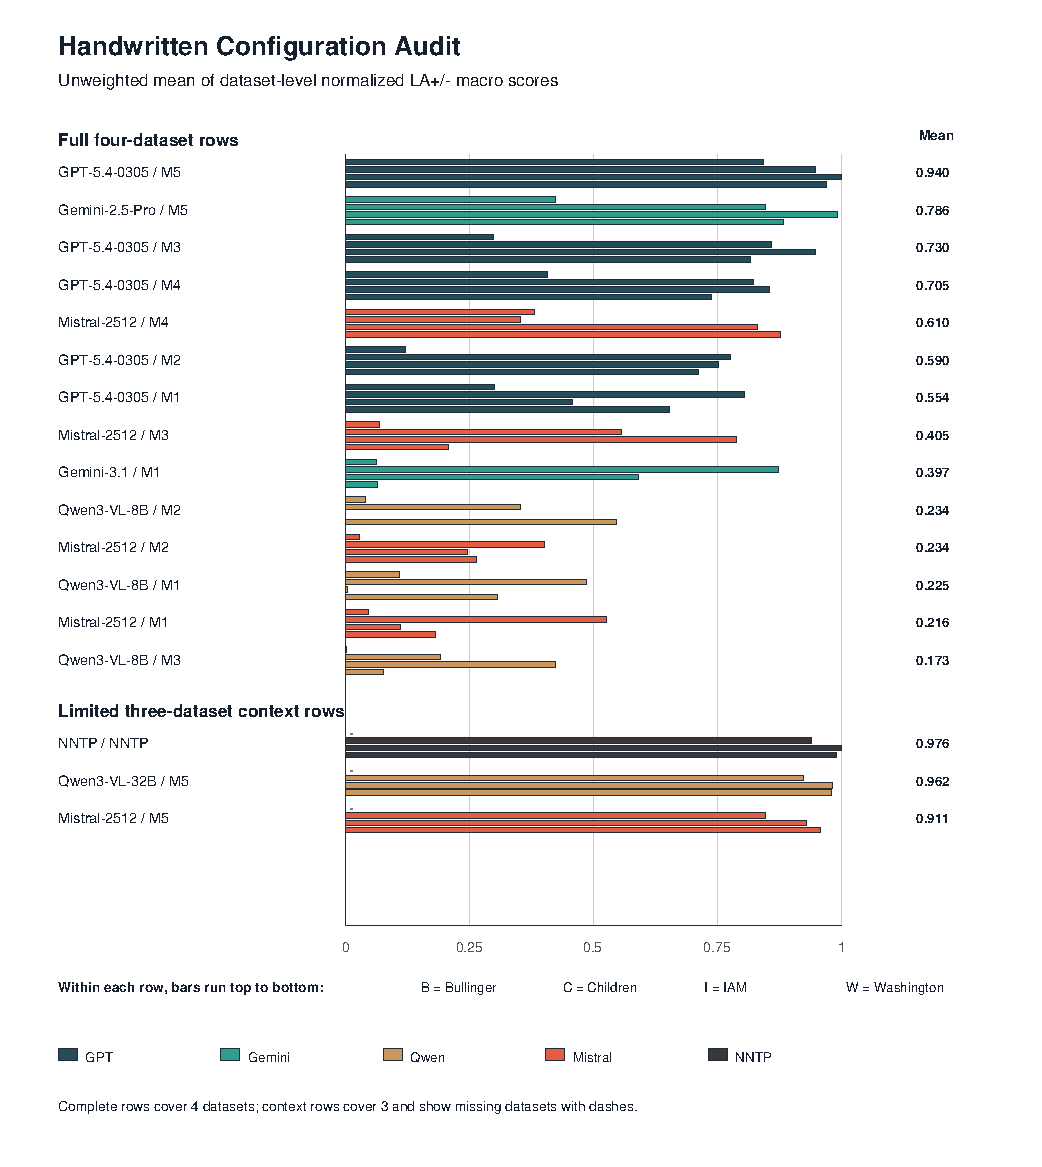
\includegraphics[width=0.98\linewidth,height=0.78\textheight,keepaspectratio]{images/ch6_results/handwritten_model_method_line_accuracy.pdf}
  \caption{Configuration audit of evaluated handwritten model/method runs. Within each row, the bars report dataset-level \LANormCombined{} macro scores in the order Bullinger, Children, IAM, and Washington; dashes mark unavailable datasets in limited context rows. The rightmost mean is the unweighted average of the represented dataset cells and is used only to order the figure. The upper block contains complete four-dataset rows, whereas the lower block contains limited three-dataset context rows. The figure summarizes configuration coverage and context; limited-coverage rows are interpreted through the caveats in the surrounding text and Appendix Table~\ref{tab:app_handwritten_model_method_overview_values}. Table~\ref{tab:exp_handwritten_main_overview} and Table~\ref{tab:exp_handwritten_controlled_model} provide the main LLM/VLM method-configuration comparisons.}
  \label{fig:exp_handwritten_llm_model_overview}
\end{figure}
\FloatBarrier

Table~\ref{tab:exp_handwritten_main_overview} condenses the LLM/VLM side of the same evidence by reporting the highest-scoring complete evaluated row for each dataset and method. This table answers RQ1 at the method-configuration level. Within the reported handwritten evaluation, M5 has the highest observed LLM/VLM macro score for Bullinger Handwritten, Children Handwritten, IAM Handwritten, and Washington Handwritten. The largest reported separation appears on Bullinger, where the M5 setup is far above the raw-output methods. IAM shows a different pattern, because OCR-conditioned M3 is already strong, and M5 reaches the ceiling.

\begin{table}[H]
  \centering
  \caption{Descriptive best-row overview for the four handwritten LLM/VLM-based datasets. Each cell reports \LANormCombined{}, the whitespace-normalized combined order-sensitive line accuracy, macro-averaged over sample IDs and formed as the mean of \LANormForward{} and \LANormReverse{} before rounding. Each dataset-method cell uses the highest-scoring complete row within the handwritten evaluation scope. The table is a descriptive overview, not an ablation or causal method ranking, because model configurations may differ across cells and the structured M4/M5 regimes include stored line-count access, repair, fallback, and projection.}
  \label{tab:exp_handwritten_main_overview}
  \footnotesize
  \setlength{\tabcolsep}{4pt}
  \renewcommand{\arraystretch}{1.08}
  \begin{tabular}{@{}l c c c c c c@{}}
    \toprule
    \textbf{Dataset} & \textbf{\(n\)} & \textbf{M1} & \textbf{M2} & \textbf{M3} & \textbf{M4} & \textbf{M5} \\
    \midrule
    Bullinger Handwritten & 59 & 0.300 & 0.120 & 0.297 & 0.406 & \textbf{0.843} \\
    Children Handwritten & 63 & 0.872 & 0.777 & 0.859 & 0.822 & \textbf{0.948} \\
    IAM & 20 & 0.589 & 0.752 & 0.948 & 0.855 & \textbf{1.000} \\
    Washington Handwritten & 20 & 0.653 & 0.711 & 0.817 & 0.883 & \textbf{0.980} \\
    \bottomrule
  \end{tabular}
  \vspace{0.35em}

  \parbox{0.82\linewidth}{\footnotesize Bold marks the highest value within each dataset row; it does not imply causal attribution. \autoref{sec:appendix_provider_mix} lists the contributing model configurations, and Table~\ref{tab:app_model_provider_aliases} centralizes the display-name aliases. The partial Bullinger \QwenThirtyTwoShort{} M5 row covers \(20/59\) samples because the university-cluster run exhausted GPU memory on larger Bullinger samples. It is preserved as an execution record, but excluded from the complete-dataset comparison and from highest-row conclusions.}
\end{table}

The result should therefore be read as the main M5 finding rather than as evidence for a monotonic method ladder. M5 combines ordered line-image evidence, OCR/HTR line text, page context, structured output, validation, and projection. The current experiments report this setup as the highest-scoring evaluated LLM/VLM-based alignment setup; they do not isolate any single component as the sole cause of the observed differences. The controlled OpenAI table below preserves the same M5 result while reducing model-configuration variation, and \autoref{sec:appendix_prompt_detail_metrics} expands the same rows with directional scores and supporting diagnostics.

The next layer narrows the comparison level. Table~\ref{tab:exp_handwritten_controlled_model} asks whether the same main result remains visible when one OpenAI model configuration is held fixed across M1--M5.

\paragraph{Controlled LLM/VLM-based checks.}
\label{sec:experimentation_controlled_checks}

Table~\ref{tab:exp_handwritten_controlled_model} is the controlled OpenAI comparison for RQ1 because it keeps the LLM/VLM side on a single complete OpenAI model configuration while preserving the five-method progression. Its purpose is not to replace the overview. It tests whether the main result remains visible after one major source of variation is removed.

\begin{table}[H]
  \centering
  \caption{Exact-model OpenAI control for the handwritten LLM/VLM-based comparison. Each cell reports \LANormCombined{}, the whitespace-normalized combined order-sensitive line accuracy, macro-averaged over sample IDs and formed as the mean of \LANormForward{} and \LANormReverse{} before rounding. All rows use \GPTFiveMarchShort{}. The structured M4 and M5 rows retain the known-count prerequisite and projection as part of the evaluated regime.}
  \label{tab:exp_handwritten_controlled_model}
  \footnotesize
  \begin{tabular}{@{}l c c c c c c@{}}
    \toprule
    \textbf{Dataset} & \textbf{Coverage} & \textbf{M1} & \textbf{M2} & \textbf{M3} & \textbf{M4} & \textbf{M5} \\
    \midrule
    Bullinger Handwritten & 59/59 & 0.300 & 0.120 & 0.297 & 0.406 & \textbf{0.843} \\
    Children Handwritten & 63/63 & 0.804 & 0.777 & 0.859 & 0.822 & \textbf{0.948} \\
    IAM & 20/20 & 0.458 & 0.752 & 0.948 & 0.855 & \textbf{1.000} \\
    Washington Handwritten & 20/20 & 0.653 & 0.711 & 0.817 & 0.737 & \textbf{0.970} \\
    \bottomrule
  \end{tabular}
  \vspace{0.35em}

  \parbox{0.82\linewidth}{\footnotesize Bold marks the highest value within each dataset row; it does not imply causal attribution. The M5 column uses the documented zero-shot context-rich M5 configuration. This table is the primary controlled LLM/VLM-based comparison because it keeps one OpenAI model configuration across M1--M5 and uses the full sample set for all four handwritten datasets; the archived M5 OpenAI shorthand is documented in Table~\ref{tab:app_model_provider_aliases}.}
\end{table}

The control table preserves the main result while changing the story about the path to it. Under the \GPTFiveMarchShort{} model configuration, the intermediate steps are clearly non-monotonic. Children drops from \(0.859\) at M3 to \(0.822\) at M4, and Washington drops from \(0.817\) at M3 to \(0.737\) at M4 before jumping to \(0.970\) at M5. Bullinger likewise shows a substantially higher M5 score, but not a smooth method ladder, since the sequence rises from \(0.120\) at M2 to \(0.297\) at M3, \(0.406\) at M4, and \(0.843\) at M5. The supported claim is therefore not monotonicity at every step; it is the specific observation that M5 has the highest observed macro score among the evaluated LLM/VLM-based methods under one OpenAI model configuration across all four datasets.

\paragraph{Takeaway.}
The handwritten tables support a narrow but consistent reading in which M5 is the highest LLM/VLM-based row in both the descriptive overview and the exact-model OpenAI control, while the order of M1--M4 changes by dataset. The tables therefore support M5 as the main result for the reported setups, not a smooth stepwise improvement claim across all methods.

\paragraph{Preliminary check: Adding one example to the prompt.}\label{sec:experimentation_one_shot_exploratory}\mbox{}\par

Before fixing the final handwritten evaluation setup, a small exploratory run tested whether the raw-output methods M1--M3 benefit from one worked example in the prompt. In this setting, each target sample was preceded by one example from the same dataset. This is often called one-shot prompting: The model receives one demonstration of the desired input-output behavior before solving the current sample.

The check was limited to GPT-5.2 and Qwen3-VL-8B and to the early M1--M3 setup. It was not run for M4 or M5 and is not part of the main M1--M5 result claims. Figure~\ref{fig:exp_one_shot_deltas} reports the change from the corresponding zero-example prompt to the one-example prompt. Positive values mean that the one-example prompt improved whitespace-normalized \LANormCombined{}; negative values mean that it reduced accuracy.

\begin{figure}[H]
  \centering
  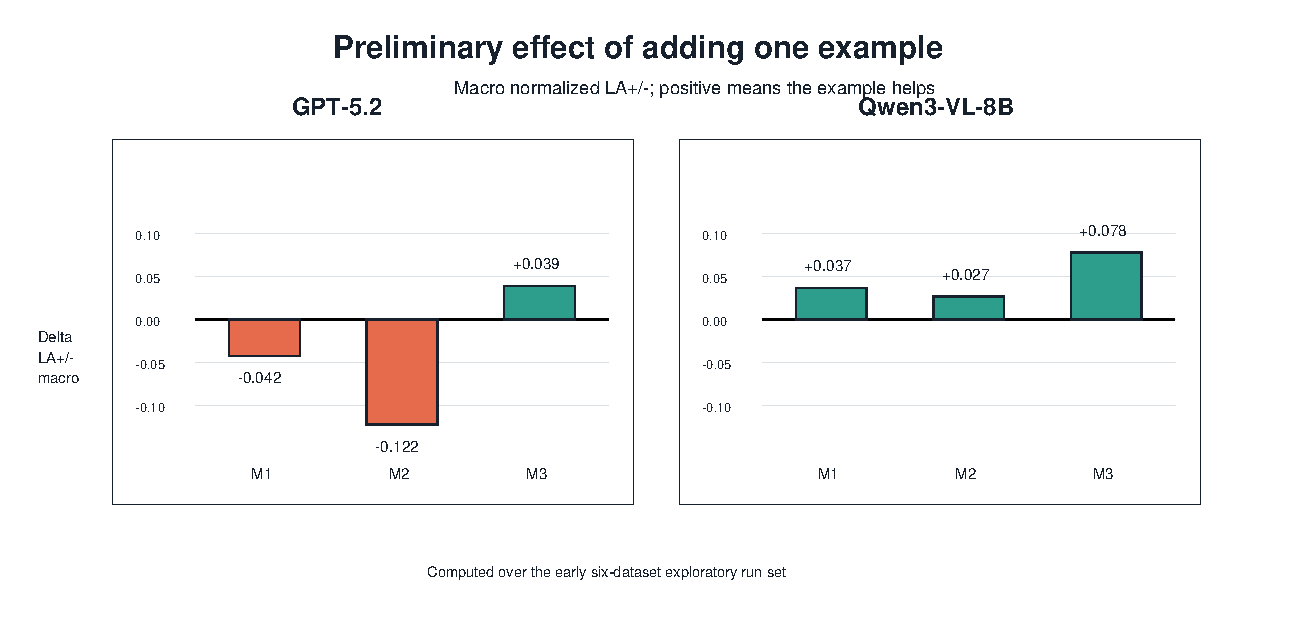
\includegraphics[width=0.88\linewidth]{images/ch6_results/exploratory_one_shot_deltas.pdf}
  \caption{Preliminary effect of adding one worked example to M1--M3 prompts. Bars show the change in whitespace-normalized \LANormCombined{} relative to the corresponding zero-example prompt for two model configurations in an early exploratory run set. Positive values indicate higher line accuracy with the example included. The check is diagnostic only and is not used in the main M1--M5 comparison.}
  \label{fig:exp_one_shot_deltas}
\end{figure}

The result is mixed. The GPT-5.2 row loses accuracy for M1 and M2 but improves for M3, while the \QwenEightShort{} row improves on all three methods from a lower early baseline. This was not a stable enough signal to justify expanding one-example prompting to the structured M4/M5 experiments. The main experiments therefore focus on the final zero-shot and context-rich structured configurations.

\subsection{Model-Configuration Robustness}
\label{sec:experimentation_provider_model_robustness}

The main RQ1 pattern survives the primary complete model-configuration control, where M5 remains the highest-scoring reported LLM/VLM-based configuration while the intermediate rankings stay model- and dataset-sensitive. This robustness check is a guardrail around the first empirical layer. Table~\ref{tab:exp_handwritten_main_overview} and the appendix duplicate in Table~\ref{tab:exp_handwritten_prompt_matrix} are descriptive because each dataset-method cell may be supplied by a different model configuration; the provenance is explicit in Table~\ref{tab:app_handwritten_prompt_provenance}, with display-name aliases centralized in Table~\ref{tab:app_model_provider_aliases}. Table~\ref{tab:exp_handwritten_controlled_model} is the primary controlled LLM/VLM progression table: It keeps one OpenAI model configuration, \GPTFiveMarchShort{}, across M1--M5 and uses the full sample set for all four handwritten datasets. The \MistralLargeShort{} matrix in Table~\ref{tab:app_mistral_fixed_provider_matrix} is stricter in provider scope, but secondary for the thesis argument because its Bullinger M5 cell is missing after the Bullinger M5 run did not complete following API errors and its absolute scores differ from the OpenAI/Qwen/Gemini rows included in the thesis evidence.

Within those results, Washington is the clearest model-sensitive case. The Washington M4 and M5 cells in Table~\ref{tab:exp_handwritten_main_overview} are supplied by \QwenEightShort{} and \QwenThirtyTwoShort{}, with \LANormCombined{} values of \(0.883\) and \(0.980\), whereas the exact OpenAI control reports \(0.737\) for M4 and \(0.970\) for M5 on the same dataset. This does not rank Qwen against OpenAI in general; it shows specifically that the selected Washington results for M4/M5 depend on the selected model configuration. The main conclusion survives the complete OpenAI control, and M5 remains the highest-scoring reported LLM/VLM-based configuration in Table~\ref{tab:exp_handwritten_controlled_model}. The intermediate order of M1--M4 remains model- and dataset-sensitive, so the thesis treats those rankings as contextual rather than as model-family effects isolated from provider and dataset variation.

\FloatBarrier

\section{Secondary Printed-Context Results}
\label{sec:experimentation_print_results}

The secondary printed context provides supporting modality evidence without changing the main handwritten answer. It extends the same newline-only evaluation target to Bullinger Print and IAM Print for the raw-output M1--M3 configurations. Because M4, M5, and NNTP were not run on the printed datasets, this section reports limited M1--M3 rows as secondary printed context rather than a full evidence-and-control progression.

\begin{table}[H]
  \centering
  \caption{Secondary printed-dataset results for the reported M1--M3 scope. Values are whitespace-normalized \LANormCombined{} macro-averages over sample IDs, reported from retained print evaluation CSV macro rows and rounded to three decimals. Each cell reports the highest-scoring complete zero-shot row for that printed dataset and method. M4, M5, and NNTP were not run on the printed datasets and are therefore not shown.}
  \label{tab:exp_print_secondary}
  \footnotesize
  \renewcommand{\arraystretch}{1.08}
  \begin{tabular}{@{}l c c c c@{}}
    \toprule
    \textbf{Dataset} & \textbf{Samples} & \textbf{M1} & \textbf{M2} & \textbf{M3} \\
    \midrule
    Bullinger Print & 10 & \textbf{0.594} (GPT-5.2) & 0.566 (GPT-5.2) & 0.115 (\MistralLargeShort{}) \\
    IAM Print & 30 & 0.917 (GPT-5.2) & 0.896 (GPT-5.2) & \textbf{0.934} (GPT-5.2) \\
    \bottomrule
  \end{tabular}
  \vspace{0.35em}

  \parbox{0.74\linewidth}{\footnotesize Bold marks the highest value within each dataset row.}
\end{table}

The two print datasets behave differently. On IAM Print, the highest stored row is already high for all three raw-output configurations, and the highest M3 row reaches \(\LANormCombinedToken=0.934\), \(\LineFOneNormToken=0.945\), and \(\CERNormToken=0.001\). Bullinger Print is lower and less stable: Its highest M1 and M2 rows reach \(\LANormCombinedToken=0.594\) and \(0.566\), while its highest M3 row falls to \(0.115\) despite \(\CERNormToken=0.009\). This reinforces the line-structure-first reading of the metric stack: Character preservation or low CER does not by itself imply that newline boundaries have been recovered well. Because the print scope lacks M4, M5, and NNTP, these rows broaden modality context but do not change the handwritten conclusion that M5 has the highest reported macro score among the evaluated LLM/VLM-based configurations in the complete main evaluation.

To compare print and handwriting without changing the main handwritten sample sets, Table~\ref{tab:exp_print_handwriting_matched_support} uses restricted support slices in which corresponding print and handwritten rows were reported. These support slices are separate from the main handwritten evaluation sets, including the representative-20 IAM Handwritten main evaluation. The table is therefore diagnostic: It compares modalities within paired support slices and does not replace the main handwritten results in Table~\ref{tab:exp_handwritten_main_overview}.

\begin{table}[H]
  \centering
  \caption{Diagnostic matched-support print--handwriting comparison for M1--M3. Values are whitespace-normalized \LANormCombined{} macro-averages over the restricted support IDs and rounded to three decimals. The support-slice denominators are \(n=10\) shared Bullinger IDs and \(n=30\) paired IAM \texttt{a01-*} forms. The table is a direct comparison within the paired support slices; it does not replace the headline handwritten sample sets used in Table~\ref{tab:exp_handwritten_main_overview}.}
  \label{tab:exp_print_handwriting_matched_support}
  \footnotesize
  \setlength{\tabcolsep}{4pt}
  \renewcommand{\arraystretch}{1.10}
  \begin{tabular}{@{}l c c c c c c@{}}
    \toprule
    \textbf{Dataset} & \shortstack{\textbf{M1}\\\textbf{handwritten}} & \shortstack{\textbf{M1}\\\textbf{print}} & \shortstack{\textbf{M2}\\\textbf{handwritten}} & \shortstack{\textbf{M2}\\\textbf{print}} & \shortstack{\textbf{M3}\\\textbf{handwritten}} & \shortstack{\textbf{M3}\\\textbf{print}} \\
    \midrule
    Bullinger & 0.148 & 0.594 & 0.083 & 0.566 & 0.066 & 0.115 \\
    IAM & 0.959 & 0.917 & 0.912 & 0.896 & 0.802 & 0.934 \\
    \bottomrule
  \end{tabular}
\end{table}

The diagnostic comparison separates two patterns. For Bullinger, print scores higher than the matched handwritten support slice for M1--M3, but Bullinger Print M3 remains much lower than Bullinger Print M1 and M2. For IAM, both modalities are strong; IAM Print peaks at M3, while the matched IAM Handwritten support remains high but peaks earlier. Since M4, M5, and NNTP were not run for the secondary printed context datasets, this direct M1--M3 comparison does not test the full evidence-and-control progression used in the main handwritten evaluation.

\FloatBarrier

\section{Comparison with NNTP}
\label{sec:experimentation_direct_nntp}

RQ2 has a close, dataset-dependent answer rather than a uniform winner. On the three datasets with thesis-side dataset-level NNTP summaries over the same sample sets, M5 is slightly ahead on Children Handwritten, tied on IAM Handwritten, and slightly behind on Washington Handwritten. Table~\ref{tab:exp_best_vs_nntp} is therefore the same-sample thesis-side comparison for Children, IAM, and Washington. Bullinger is treated separately because its deterministic comparison is made against the published Bullinger alignment baseline rather than against a full \(59\)-sample thesis-side NNTP run.

\begin{table}[H]
  \centering
  \caption{Same-sample NNTP comparison for Children, IAM, and Washington. Values are whitespace-normalized \LANormCombined{} macro-averages over sample IDs. LLM/VLM rows use the highest-scoring complete reported M5 row per dataset; NNTP rows are thesis-side summaries or the legacy IAM run.}
  \label{tab:exp_best_vs_nntp}
  \footnotesize
  \renewcommand{\arraystretch}{1.08}
  \begin{tabularx}{\linewidth}{@{}Y c Y c Y c c@{}}
    \toprule
    \textbf{Dataset} & \textbf{Samples} & \textbf{LLM/VLM} & \(\mathbf{\LANormCombinedToken}\) & \textbf{NNTP setup} & \(\mathbf{\LANormCombinedToken}\) & \(\mathbf{\Delta}\) \\
    \midrule
    Children Handwritten & 63 & M5 / \GPTFiveShort{} & \textbf{0.948} & cross-validation macro (3-fold) & 0.939 & +0.009 \\
    IAM & 20 & M5 / \GPTFiveShort{} & \textbf{1.000} & legacy single run & \textbf{1.000} & 0.000 \\
    Washington Handwritten & 20 & M5 / \QwenThirtyTwoShort{} & 0.980 & cross-validation macro (2-fold) & \textbf{0.990} & -0.009 \\
    \bottomrule
  \end{tabularx}
  \vspace{0.35em}

  \parbox{0.96\linewidth}{\footnotesize Bold marks the higher value within each dataset row; ties bold both values. It is not a significance claim. Paired sample-level reconstruction gives Children \(4\) LLM/VLM wins, \(2\) NNTP wins, \(57\) ties, and \(6\) non-tied pairs; IAM \(0\) wins for either side, \(20\) ties, and \(0\) non-tied pairs; and Washington \(2\) LLM/VLM wins, \(4\) NNTP wins, \(14\) ties, and \(6\) non-tied pairs. NNTP aligns recognizer labels after symbol-inventory preprocessing rather than the untouched transcription.}
\end{table}

The comparison is direct in its metric target because both sides are scored as newline-only line reconstructions, while the implemented regimes differ. M5 uses prompts, structured controls, and projection that can restore the fixed transcription before scoring, whereas NNTP searches a forced-alignment path over recognizer-derived CTC evidence rather than producing free-form text \thesiscite{peer2025ctcBullingerAlignment}. With the preprocessing limit recorded in the table note, line accuracy is the main shared surface; character-level readings against M1--M5 retain the NNTP symbol-filtering condition summarized in Table~\ref{tab:app_nntp_symbol_filter_audit}.

At sample level, the comparison is dominated by ties. Children has 4 LLM/VLM wins, 2 NNTP wins, and 57 ties; IAM has 20 ties; Washington has 2 LLM/VLM wins, 4 NNTP wins, and 14 ties. The few non-tied cases do not support a directional claim. A two-sided exact sign test gives \(p = 0.688\) for Children (\(4\) vs.\ \(2\), \(n=6\) non-tied pairs) and \(p = 0.688\) for Washington (\(2\) vs.\ \(4\), \(n=6\) non-tied pairs), while IAM has no non-tied pairs to test. The sample-level evidence therefore supports closeness and tie-dominance rather than a clear advantage for either approach.

\paragraph{Takeaway.}
The same-sample NNTP comparison is close rather than one-sided. On the matched handwritten comparison sets, Children slightly favors M5, IAM ties, and Washington slightly favors NNTP; the paired counts are dominated by ties. Bullinger is outside this matched claim except for the subset-level context below. Within this comparison, the evidence supports a close, tie-dominated, and dataset-dependent RQ2 interpretation.

\FloatBarrier

\paragraph{Bullinger published-baseline context.}
\label{sec:experimentation_bullinger_contextual}

Bullinger remains part of the NNTP discussion because the recent Bullinger alignment study reports a deterministic baseline for the same task family \thesiscite{peer2025ctcBullingerAlignment}. Unlike Children, IAM, and Washington, the comparison is not a full thesis-side NNTP run over the \(59\)-sample thesis denominator. It is a subset-level comparison against the published Bullinger baseline.

Table~\ref{tab:exp_bullinger_contextual} reports this comparison using raw forward line accuracy \(\LAForward\) to stay close to the published baseline. Subset~1 is directly comparable because the thesis subset matches the published inventory at the letter and line level. Subset~2 is contextual because the thesis and paper inventories differ.

\begin{table}[t]
  \centering
  \caption{Bullinger published-baseline comparison against the published NNTP baseline. Values are raw \LAForward{} scores, not whitespace-normalized \LANormForward{} scores; thesis-side values are macro-averaged over sample IDs, while the paper values are the published subset-level NNTP scores. All thesis-side Bullinger runs use the same author-provided subset version; direct comparison to the paper is possible for Subset~1 but remains contextual for Subset~2.}
  \label{tab:exp_bullinger_contextual}
  \footnotesize
  \renewcommand{\arraystretch}{1.08}
  \begin{tabularx}{\linewidth}{@{}Y c Y c c c@{}}
    \toprule
    \textbf{Subset} & \textbf{Thesis sample set} & \textbf{Highest-scoring thesis LLM/VLM configuration} & \(\mathbf{\LAForwardToken}\) & \textbf{Paper sample set} & \(\mathbf{\LAForwardToken}\) \\
    \midrule
    Subset~1 & 20 letters / 902 lines & M5 / \GPTFiveShort{} & 0.821 & 20 letters / 902 lines & \textbf{0.861} \\
    Subset~2 & 39 letters / 1633 lines & M5 / \GPTFiveShort{} & \textbf{0.865} & 49 letters / 1486 lines & 0.773 \\
    \bottomrule
  \end{tabularx}
  \vspace{0.35em}

  \parbox{0.96\linewidth}{\footnotesize Bold marks the higher \LAForward{} value within each subset row. Subset~1 is direct because it matches at the letter and line level; Subset~2 is contextual because the thesis and paper inventories differ.}
\end{table}

\FloatBarrier

The result is mixed in a precise way. On Subset~1, the published NNTP result is higher than the thesis M5 result. On Subset~2, the thesis M5 value is higher, but this comparison is contextual because the inventories differ. The Bullinger evidence therefore does not support a single full-dataset M5-versus-NNTP winner. It shows that NNTP remains stronger on the directly matched subset, while M5 is higher only in the contextual Subset~2 comparison \thesiscite{peer2025ctcBullingerAlignment}.

\section{Output Control and Fixed-Transcription Validity}
\label{sec:experimentation_output_control_audit}

RQ3 asks a validity question before an accuracy question. The central issue is whether the scored output is a newline plan over the supplied transcription rather than a generated transcription. The structured M5 traces show that this control path works reliably in the archived context-rich handwritten runs. Across \(162/162\) samples, the first strict JSON response already satisfied the exact-count requirement for \(157\) samples. The remaining cases were handled by the repair, loose-recovery, or deterministic-fallback paths; all such events occur in Bullinger. After the selected boundary plan is projected onto the untouched transcription, the final scored string preserves the fixed character stream.

Table~\ref{tab:app_m5_trace_event_counts} gives the corresponding M5 event-count audit by dataset and explains how M5 combines generative evidence with fixed-transcription validity: Model-proposed lines are treated as boundary evidence, not as final text.

\begin{table}[H]
  \centering
  \caption{Structured output-validity events archived for the complete \GPTFiveShort{} context-rich M5 configuration in the reported handwritten evaluation set. These are event counts rather than whitespace-normalized metric values or sample-ID macro-averages.}
  \label{tab:app_m5_trace_event_counts}
  \footnotesize
  \renewcommand{\arraystretch}{1.08}
  \begin{tabular}{@{}l c c c c c c c c@{}}
    \toprule
    \textbf{Dataset} & \textbf{Samples} & \shortstack{\textbf{1st}\\\textbf{JSON}} & \textbf{Repair} & \textbf{Loose} & \textbf{Fallback} & \shortstack{\textbf{Final proj.}\\\textbf{mode}} & \textbf{Fail} & \textbf{Missing} \\
    \midrule
    Bullinger Handwritten & 59 & 54 & 2 & 3 & 3 & 39 & 0 & 0 \\
    Children Handwritten & 63 & 63 & 0 & 0 & 0 & 58 & 0 & 0 \\
    IAM (20-form) & 20 & 20 & 0 & 0 & 0 & 20 & 0 & 0 \\
    Washington Handwritten & 20 & 20 & 0 & 0 & 0 & 19 & 0 & 0 \\
    \bottomrule
  \end{tabular}
  \vspace{0.35em}

  \parbox{0.88\linewidth}{\footnotesize\raggedright ``1st JSON'' counts samples whose first strict parse already satisfied the exact-count JSON requirement. ``Repair'' counts samples whose first strict parse failed but whose repair response then succeeded. ``Loose'' counts traces that recovered a usable boundary plan from non-strict model lines (\texttt{reconciled\_model\_lines} or \texttt{quality\_repair\_recovered}). ``Fallback'' marks deterministic fallback projection. ``Final proj. mode'' counts traces whose final logged resolution mode is \texttt{projection\_from\_model\_lines}; candidate projections evaluated inside \texttt{reference\_alignment\_selection} are not exposed as a separate boolean in the stored schema and are therefore not double-counted here. ``Missing'' \(=0\) indicates complete trace availability for this M5 audit layer. The event columns are trace flags rather than a mutually exclusive partition of samples; a sample may satisfy more than one condition, for example by parsing successfully and still being projected, or by passing through repair before fallback. More broadly, the M5 scored string is not raw returned text: Accepted, recovered, or fallback boundary plans may be projected back onto the untouched transcription before evaluation.}
\end{table}
\FloatBarrier

The event-count audit is reported for M5 because the final structured M5 runs have complete trace records for the handwritten evaluation. M4 follows the same structured-output principle and remains part of the score tables, but its trace records are not complete enough for a parallel event-count summary. The M5 event counts should therefore be read as evidence for the final structured configuration, not as inferred totals for M4.

The same distinction is visible in a simpler line-count diagnostic. Before asking whether a boundary is placed exactly, Table~\ref{tab:exp_line_count_drift} asks whether the output has the right number of lines at all. For each LLM/VLM scored prediction, \(\Delta L\) is defined as the number of predicted lines minus the number of ground truth lines after splitting the prediction and ground truth text on newlines; \MeanAbsLineDelta{} denotes the corresponding mean absolute line-count difference. The table reports all canonical scored rows for which prediction and ground truth text could both be reconstructed; this set is complete for the scored rows included here (\(2633/2633\)).

\begin{table}[H]
  \centering
  \caption{Line-count drift in documented handwritten LLM/VLM rows. This is not a whitespace-normalized accuracy table: Predicted and ground truth line counts are summed over scored rows whose prediction and ground truth text could both be reconstructed, repeated samples across model configurations remain separate observations, and \MeanAbsLineDelta{} is averaged over those rows rather than macro-averaged over unique sample IDs.}
  \label{tab:exp_line_count_drift}
  \footnotesize
  \renewcommand{\arraystretch}{1.08}
  \begin{tabular}{@{}l c r r c r r r@{}}
    \toprule
    \textbf{Method} & \textbf{Rows} & \textbf{Pred. lines} & \textbf{GT lines} & \(\mathbf{\MeanAbsLineDeltaToken}\) & \(\mathbf{\Delta L=0}\) & \textbf{Under} & \textbf{Over} \\
    \midrule
    M1 & 648/648 & 10894 & 15060 & 7.630 & 275 & 295 & 78 \\
    M2 & 506/506 & 9570 & 11951 & 5.911 & 244 & 197 & 65 \\
    M3 & 506/506 & 6334 & 11951 & 11.204 & 218 & 271 & 17 \\
    M4 & 423/423 & 10848 & 10901 & 0.125 & 399 & 24 & 0 \\
    M5 & 550/550 & 10426 & 10430 & 0.007 & 546 & 4 & 0 \\
    \bottomrule
  \end{tabular}
  \vspace{0.35em}

  \parbox{0.96\linewidth}{\footnotesize Under and over count rows with fewer or more predicted lines than the ground truth. Aggregated across methods, the raw-output rows M1--M3 have \MeanAbsLineDelta{} \(=8.195\) over \(1660\) rows, whereas the structured rows M4--M5 have \MeanAbsLineDelta{} \(=0.059\) over \(973\) rows.}
\end{table}

Table~\ref{tab:exp_line_count_drift} supports RQ3 as output-validity evidence rather than as an independent accuracy claim. M1--M3 frequently under-segment or over-segment because the raw returned text must both copy the transcription and choose the global number of output lines. Reliable ordered line metadata is an operational prerequisite of M4/M5 as evaluated, and their configurations validate against the stored cardinality before repairing, recovering, falling back, or projecting before scoring. In the handwritten datasets used here, the stored \texttt{ocr\_lines} cardinality matches the ground-truth line count, so the structured configurations test boundary assignment under known-count staging rather than blind line-count prediction. Their low \MeanAbsLineDelta{} should therefore be interpreted as output validity under that condition, not as evidence of page-side line-count inference.

This analysis also defines the scope of the RQ3 evidence. The equivalent M4 event-count trace layer is incomplete: The appendix documents the M4 control logic, but not same-sample M4 event totals across the handwritten datasets. M4 event totals are therefore not reported from traces, and they should not be inferred from the M5 layer or from code-level behavior alone. Consequently, Chapter~7 can answer RQ3 at the configuration and output-validity level: Structured output control is practically important because it makes the scored LLM/VLM outputs valid under the fixed-transcription newline-only task definition. Isolated effects of strict JSON, repair, fallback, and projection remain future ablation questions because those controls co-vary with the known-count staging, evidence scaffolds, crop provenance, and provider behavior.

\paragraph{Takeaway.}
The output-control evidence shows a validity difference before it shows an accuracy difference: M1--M3 often return the wrong number of lines, whereas M4 and M5 are evaluated after exact-count validation, possible repair or fallback, and projection under known-count staging. This supports the fixed-transcription validity claim for the structured configurations, with component-level attribution left to targeted ablation work.

\section{Qualitative Error Analysis}
\label{sec:experimentation_qualitative}

The final empirical layer moves from score tables to prediction-level mechanisms. It does not replace the aggregate tables; it explains why their patterns are plausible by tracing how line-count drift, positional shifts, OCR noise, structured fallback, and NNTP local boundary choices appear in stored predictions.

\FloatBarrier

\subsection{Method-Level Error Mechanisms}
\label{sec:experimentation_method_weaknesses}

The mechanism-level reading is that the configurations fail for different reasons, so the aggregate RQ answers should be read as configuration-level evidence rather than as isolated component effects. The prediction- and trace-level analysis of stored artifacts turns the preceding score differences into method-level mechanisms. Table~\ref{tab:exp_method_weakness_mechanisms} is the analytical bridge between aggregate scores and individual excerpts: It reads each row through the same questions--what helps, what fails, which mechanism is visible, and how that mechanism bounds the research-question answer. Appendix Table~\ref{tab:app_method_weakness_evidence} keeps the counted rows, named sample IDs, trace evidence, and longer mechanism notes that support this compact reading. The main-text table therefore summarizes secondary analysis of stored artifacts; appendix counts support traceability, while named samples remain illustrative rather than prevalence estimates.

\begin{table}[!htbp]
  \centering
  \caption{Analytical summary of observed method strengths, limitations, and likely error mechanisms in the documented prediction- and trace-level analysis. Appendix Table~\ref{tab:app_method_weakness_evidence} preserves the counted evidence, sample IDs, trace details, and longer explanations behind these summaries. For NNTP, character-level interpretation preserves the NNTP preprocessing caveat.}
  \label{tab:exp_method_weakness_mechanisms}
  \footnotesize
  \setlength{\tabcolsep}{3pt}
  \renewcommand{\arraystretch}{1.10}
  \begin{tabularx}{\linewidth}{@{}>{\raggedright\arraybackslash}p{0.075\linewidth}>{\raggedright\arraybackslash}p{0.20\linewidth}>{\raggedright\arraybackslash}p{0.21\linewidth}>{\raggedright\arraybackslash}p{0.25\linewidth}Y@{}}
    \toprule
    \textbf{Method} & \textbf{Main strength} & \textbf{Observed limitation} & \textbf{Likely mechanism} & \textbf{Implication} \\
    \midrule
    M1 & Useful when the raw response respects the fixed character stream. & Weak raw-output constraint; omissions, additions, character drift, and count drift. & Copying and segmenting happen in one unconstrained generation; early drift shifts the sequence. & Image evidence helps RQ1 when the fixed-transcription requirement holds; motivates RQ3 control. \\
    \addlinespace[0.35em]
    M2 & OCR/HTR can rescue image-only failures when hint lineation is close. & OCR noise or chunk mismatch can hurt relative to M1. & The model may follow a noisy hint or mispaired chunk over the fixed transcription. & OCR/HTR is a noisy structural hint, not monotonic extra evidence. \\
    \addlinespace[0.35em]
    M3 & Strong when OCR line order is already close to the ground truth. & Cannot correct OCR-side boundary or ordering mistakes; often under-segments. & The text hint can be enough on OCR-friendly pages, but no image signal remains. & Evidence quality matters more than simply adding channels. \\
    \addlinespace[0.35em]
    M4 & Usually controls line count and preserves the transcription after projection. & Correct count can still leave wrong order-sensitive boundaries; not consistently above M3. & Structured OCR scaffolds constrain form but can also lock in flawed OCR splits. & RQ3 validity improves, but RQ1 should not treat M4 as a guaranteed accuracy gain. \\
    \addlinespace[0.35em]
    M5 & Highest reported LLM/VLM macro score overall; projection preserves the fixed stream. & Counterexamples remain around repair, fallback, hyphenation, and short-line anchors. & The evaluated context-rich line-image configuration usually anchors boundaries, but local decisions and trace modes remain entangled. & Supports the highest-scoring evaluated configuration, not an every-sample or component-level causal claim. \\
    \addlinespace[0.35em]
    NNTP & Competitive deterministic forced alignment on matched datasets. & Local merge/split errors remain; character comparison has the preprocessing caveat. & Fixed count and CTC evidence constrain the search, but local boundary placement can still shift. & RQ2 is close and dataset-dependent; line accuracy is primary. \\
    \bottomrule
  \end{tabularx}
\end{table}

Read across the rows, the table gives a compact explanation for the non-monotonic LLM/VLM progression in Tables~\ref{tab:exp_handwritten_main_overview} and~\ref{tab:exp_handwritten_controlled_model}. Extra evidence helps where it is both structurally informative and brought under the fixed-transcription requirement; otherwise it can add a new failure channel. This is why the qualitative analysis first names configuration-level mechanisms and only then turns to individual excerpts.

The M2 pattern explains why adding OCR/HTR hints does not automatically improve M1. In the same-model pairs, M2 is more often worse than better relative to M1, even though individual samples show clear help from OCR/HTR lineation. The mechanism visible in the predictions is not a contradiction: M2 adds a second structural signal but still scores raw returned text, and that signal can be noisy or mismatched to the image/transcription chunk presented to the model. M3 shows the complementary case. When OCR/HTR line order is already close to the ground truth, as in the IAM plateau case, the text-only prompt can recover the lineation without needing page images; when OCR/HTR boundaries are wrong, M3 has no visual fallback.

M4 and M5 separate output validity from boundary accuracy. Two Washington sample IDs are used below as named diagnostic cases. Washington 307 is the case in Table~\ref{tab:exp_f1_la_divergence_cases} where M4 preserves the text but splits the opening header/date in a way that shifts the order-sensitive line sequence. Washington 270 is the case in Table~\ref{tab:exp_linebreak_comparison} where the selected M5 row enters fallback after repair and over-splits the hyphenated \texttt{Recrui-\textbackslash nting} boundary; the matched NNTP row preserves the ground truth split. These cases illustrate sample-level mechanisms and are not prevalence estimates. M4's stronger JSON and line-count scaffold explains why it usually preserves the expected count, but the Washington 307 case shows that a correct count and high exact-line F1 can coexist with order-sensitive failure. M5 adds the evaluated context-rich line-image configuration and has the highest reported overall LLM/VLM macro scores, yet the stored predictions and traces still contain counterexamples. The Washington 270 case shows that the selected M5 row can trail M3 on an individual page. Fallback and repair-attempt trace slices have lower average \LANormCombined{}, and local hyphen or short-line placements remain visible error mechanisms. These trace associations are descriptive because trace mode co-varies with dataset, provider, and sample difficulty.

The NNTP row carries the RQ2 result into the mechanism layer. The same-sample table gives small dataset-level differences, and the paired counts are dominated by ties. Prediction-level evidence explains why: NNTP often has the right line count and stable text-side behavior, but it can still merge two neighboring ground-truth lines or split at the wrong local position. With NNTP-side symbol filtering kept in view, the shared line-accuracy metric family remains the primary comparison level.

\FloatBarrier

\subsection{Excerpt-Backed Qualitative Cases}
\label{sec:experimentation_qualitative_cases}

The excerpt-backed examples narrow the mechanism view to concrete line-break behavior. Their purpose is explanatory: The aggregate tables and paired same-sample NNTP counts carry the average-behavior claims, while the examples show how nearly perfect character preservation can coexist with wrong line structure, why OCR hints can both help and mislead, why IAM can plateau across methods, and how an NNTP-favored Washington case can arise. Each example is anchored by the same per-sample metrics used throughout the chapter, especially \LANormCombined, \LineFOneNorm, and \CERNorm.

A more specific diagnostic split appears when \LineFOneNorm{} and \LANormCombined{} disagree. As defined in \autoref{sec:experimentation_line_alignment_metrics}, normalized exact-line F1 is order-insensitive: It asks whether full normalized ground-truth line strings can be matched somewhere in the prediction. By contrast, \LANormCombined{} is order-sensitive and directional. Table~\ref{tab:exp_f1_la_divergence_cases} is therefore not a gallery of unusual failures; it isolates the metric mechanism behind several aggregate readings. Many line strings can be present as exact strings, but one omitted line or one local split can move the sequence out of positional agreement. These rows explain why the thesis reports both metric families.

\begin{table}[!htbp]
  \centering
  \caption{Diagnostic cases where normalized exact-line F1 is high while normalized bidirectional order-sensitive line accuracy is much lower. Values are whitespace-normalized per-sample metrics, not macro-averages over sample IDs; explanations are based on the corresponding stored predictions and ground-truth texts.}
  \label{tab:exp_f1_la_divergence_cases}
  \footnotesize
  \renewcommand{\arraystretch}{1.12}
  \setlength{\tabcolsep}{3pt}
  \begin{tabularx}{\linewidth}{@{}>{\raggedright\arraybackslash}p{0.15\linewidth}>{\raggedright\arraybackslash}p{0.18\linewidth}c c c Y@{}}
    \toprule
    \textbf{Dataset/sample} & \textbf{Method/model configuration} & \(\mathbf{\LANormCombinedToken}\) & \(\mathbf{\LineFOneNormToken}\) & \(\mathbf{\CERNormToken}\) & \textbf{Mechanism} \\
    \midrule
    Bullinger 12517 & M1 / \GPTFiveMarchShort{} & 0.000 & 0.909 & 0.006 & The opening identifier line is omitted; most remaining line strings still occur, but the prediction begins at the second ground-truth line and never regains positional agreement. \\
    \addlinespace[0.25em]
    Bullinger 11084 & M1 / \GPTFiveMarchShort{} & 0.484 & 0.984 & 0.003 & A single missing opening identifier gives forward accuracy \(0.000\), while reverse accuracy remains \(0.969\) because the tail realigns almost perfectly. \\
    \addlinespace[0.25em]
    Washington 307 & M4 / \GPTFiveMarchShort{} & 0.000 & 0.839 & 0.000 & The structured scaffold splits the opening header/date into separate lines, shifting the following sequence even though most normalized line strings are still recovered. \\
    \addlinespace[0.25em]
    Washington 305 & M3 / \GPTFiveMarchShort{} & 0.485 & 0.985 & 0.002 & The standalone \texttt{GW} line is dropped near the end; nearly all line strings remain, but the suffix is shifted by one line. \\
    \bottomrule
  \end{tabularx}
\end{table}

Table~\ref{tab:exp_f1_la_divergence_cases} isolates the order-sensitive metric contrast. The final qualitative table then broadens from that contrast to the five mechanisms needed for the chapter's argument.

The selected qualitative cases cover content-preserving structural failure, OCR-noise recovery, high exact-line F1 with low line accuracy, plateau or tie behavior, and a boundary case in which the matched M5 row is beaten by NNTP after a logged M5 fallback trace. Table~\ref{tab:exp_linebreak_comparison} is a mechanism guide rather than an appendix substitute: It shows which comparison each case illustrates, which metrics make the mechanism visible, and where the longer excerpt evidence can be checked. Longer line-break excerpts are preserved in Appendix Tables~\ref{tab:app_qualitative_excerpt_blocks} and~\ref{tab:app_qualitative_ocr_excerpt}. Figures~\ref{fig:exp_qualitative_input_washington} and~\ref{fig:exp_qualitative_input_children} show two corresponding source images.

\providecommand{\excerptnl}{\mbox{\texttt{\textbackslash n}}}
\begin{table}[!htbp]
  \centering
  \caption{Analytical guide to the selected qualitative cases. The metrics column uses whitespace-normalized per-sample values, not macro-averages over sample IDs: \LANormCombined{} denotes normalized bidirectional order-sensitive line accuracy, \LineFOneNorm{} denotes normalized exact-line F1, and \CERNorm{} denotes normalized character error rate. Full excerpt blocks with explicit line-break markers are preserved in Appendix Tables~\ref{tab:app_qualitative_excerpt_blocks} and~\ref{tab:app_qualitative_ocr_excerpt}.}
  \label{tab:exp_linebreak_comparison}
  \scriptsize
  \renewcommand{\arraystretch}{1.08}
  \setlength{\tabcolsep}{2pt}
  \begin{tabularx}{\linewidth}{@{}>{\raggedright\arraybackslash}p{0.15\linewidth}>{\raggedright\arraybackslash}p{0.19\linewidth}>{\raggedright\arraybackslash}p{0.34\linewidth}Y@{}}
    \toprule
    \textbf{Dataset/sample} & \textbf{Role} & \textbf{Compared method/model configurations and metrics} & \textbf{Mechanism} \\
    \midrule
    Washington 304 & Content-preserving structural failure & M3 / \GPTFiveMarchShort{}: \(\LANormCombinedToken=0.338\), \(\LineFOneNormToken=0.708\), \(\CERNormToken=0.000\)\par M5 / \GPTFiveShort{}: \(\LANormCombinedToken=1.000\), \(\LineFOneNormToken=1.000\), \(\CERNormToken=0.000\) & M3 preserves the character stream but collapses the opening partition into fewer metric lines; the M5 projection row restores the line count and opening boundaries. \\
    \addlinespace[0.35em]
    Children \texttt{3B\_19\_2-3} & OCR-noise recovery & M2 / \GPTFiveMarchShort{}: \(\LANormCombinedToken=0.286\), \(\LineFOneNormToken=0.286\), \(\CERNormToken=0.190\)\par M3 / \GPTFiveMarchShort{}: \(\LANormCombinedToken=0.714\), \(\LineFOneNormToken=0.714\), \(\CERNormToken=0.164\)\par M5 / \GPTFiveShort{}: \(\LANormCombinedToken=1.000\), \(\LineFOneNormToken=1.000\), \(\CERNormToken=0.000\) & The OCR-conditioned rows lose or normalize the diplomatic \texttt{\&} annotation and related line text; the M5 row projects a line-image boundary plan back onto the fixed transcription. \\
    \addlinespace[0.35em]
    Bullinger 12517 & High exact-line F1 but low line accuracy & M1 / \GPTFiveMarchShort{}: \(\LANormCombinedToken=0.000\), \(\LineFOneNormToken=0.909\), \(\CERNormToken=0.006\)\par M5 / \GPTFiveShort{}: \(\LANormCombinedToken=1.000\), \(\LineFOneNormToken=1.000\), \(\CERNormToken=0.000\) & The M1 row drops the opening identifier line, so many line strings still match as a multiset but the positional line sequence never aligns. \\
    \addlinespace[0.35em]
    IAM \texttt{p06-042} & Plateau / tie behavior & M3 / \GPTFiveMarchShort{}, M4 / \GPTFiveMarchShort{}, M5 / \GPTFiveShort{}, and NNTP / NNTP all report \(\LANormCombinedToken=1.000\), \(\LineFOneNormToken=1.000\), \(\CERNormToken=0.000\). & The OCR-grounded and forced-alignment evidence already matches the ground-truth lineation, so the richer M5 row adds no measurable sample-level gain. \\
    \addlinespace[0.35em]
    Washington 270 & M5 boundary case, NNTP-favored matched case, and documented fallback trace & M3 / \GPTFiveMarchShort{}: \(\LANormCombinedToken=0.935\), \(\LineFOneNormToken=0.935\), \(\CERNormToken=0.002\)\par M5 / \QwenThirtyTwoShort{}: \(\LANormCombinedToken=0.871\), \(\LineFOneNormToken=0.871\), \(\CERNormToken=0.002\); trace \texttt{fallback\_projection} after \texttt{initial+repair}\par NNTP / NNTP: \(\LANormCombinedToken=1.000\), \(\LineFOneNormToken=1.000\), \(\CERNormToken=0.000\) & The selected Washington M5 row locally over-splits hyphenated \texttt{Recrui-\textbackslash nting} as \texttt{Recrui\textbackslash n- ting}; the matched NNTP row keeps the ground-truth split. \\
    \bottomrule
  \end{tabularx}
\end{table}

\FloatBarrier

\paragraph{Content can be correct while line structure is still wrong.}
A central mechanism is content-preserving structural failure. Washington sample 304 is the cleanest illustration of why this thesis separates structural accuracy from character accuracy; it is shown with line overlay in Figure~\ref{fig:exp_qualitative_input_washington}, summarized in the first row of Table~\ref{tab:exp_linebreak_comparison}, and excerpted fully in Appendix Table~\ref{tab:app_qualitative_excerpt_blocks}. On this sample, the selected M3/\GPTFiveMarchShort{} row already achieves \(\CERNormToken=0.000\), but its \LANormCombined{} remains at \(0.338\) and \(\LineFOneNormToken=0.708\); M4/\GPTFiveMarchShort{} rises to \(\LANormCombinedToken=\LineFOneNormToken=0.941\) with \(\CERNormToken=0.000\), and M5 reaches \(\LANormCombinedToken=\LineFOneNormToken=1.000\) with \(\CERNormToken=0.000\). The page therefore reads correctly at the character level long before it is segmented correctly at the line level. This is a case in which the reported structured setups with ordered OCR scaffolds and then line-image anchors improve the line partition, without isolating either evidence source as the sole cause.

\begin{figure}[H]
  \centering
  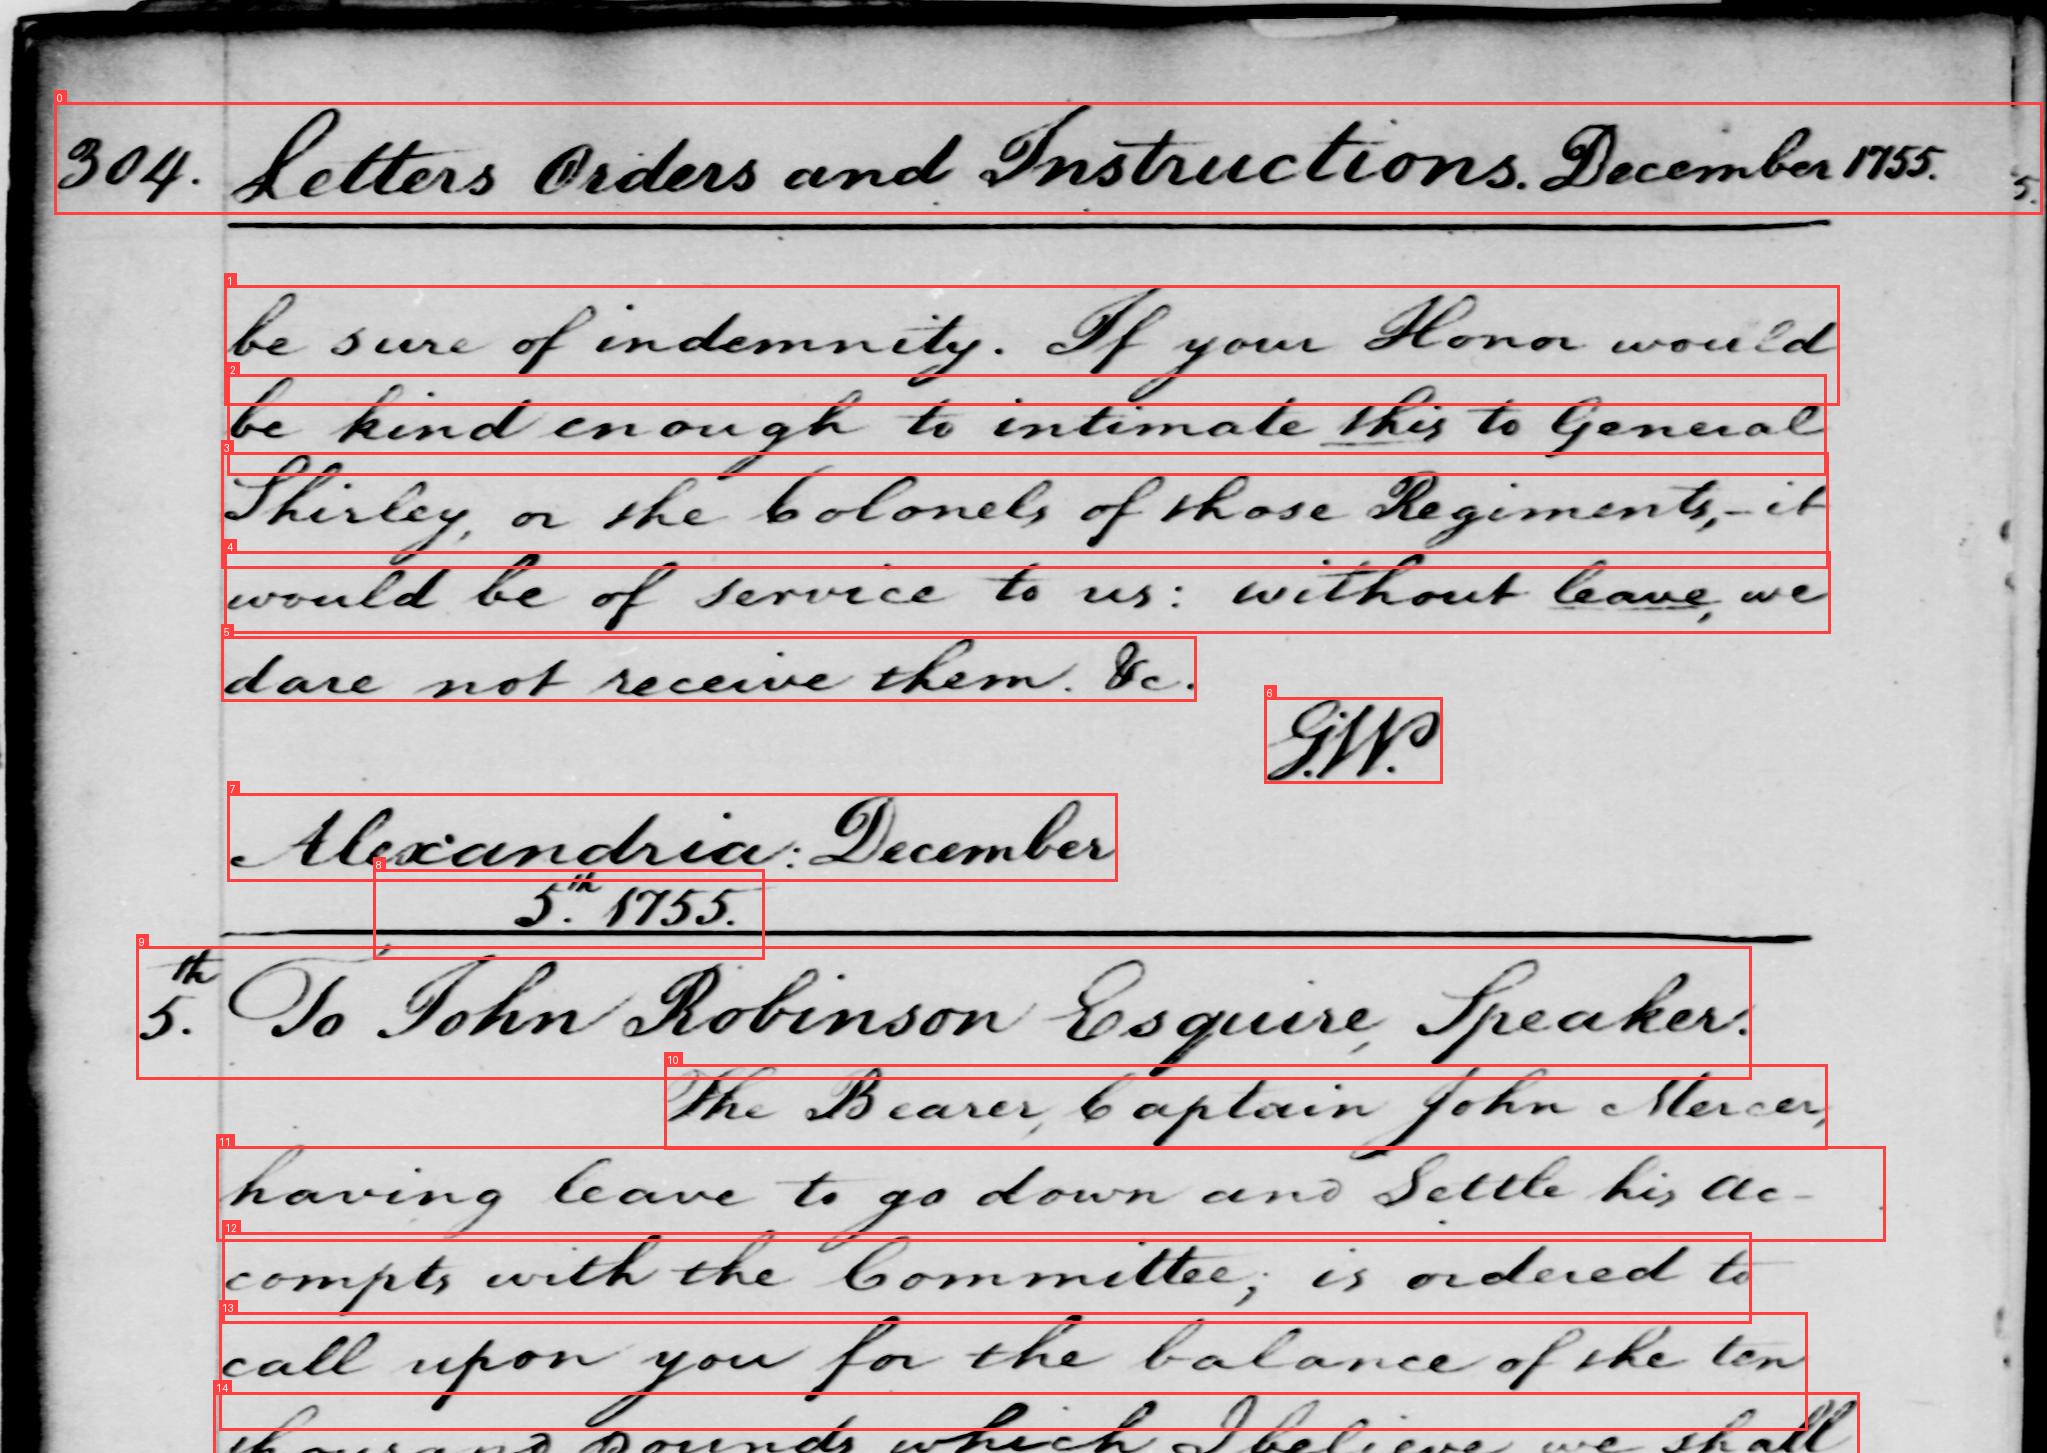
\includegraphics[width=0.92\linewidth]{images/pdf_optimized/ch6_washington_304_overlay_crop.jpg}
  \caption{Cropped upper-region view of Washington sample 304 with OCR-line overlay. The crop shows the opening line scaffold discussed in the first row of Table~\ref{tab:exp_linebreak_comparison}, the full excerpt in Appendix Table~\ref{tab:app_qualitative_excerpt_blocks}, and the first qualitative paragraph. The example illustrates that the opening-line partition remains structurally relevant even when the selected M3 row already preserves the character content.}
  \label{fig:exp_qualitative_input_washington}
\end{figure}

\needlines{8}
\paragraph{Illustrative OCR-noise recovery.}
OCR-noise recovery gives a complementary mechanism. Children sample \texttt{3B\_19\_2-3}, shown as a cropped detail in Figure~\ref{fig:exp_qualitative_input_children} and excerpted in Appendix Table~\ref{tab:app_qualitative_ocr_excerpt}, is included as an \emph{illustrative} OCR-noise example rather than as a typical Children sample. Here M2 reaches \(\LANormCombinedToken=\LineFOneNormToken=0.286\) with \(\CERNormToken=0.190\), M3 improves to \(0.714\) on both line metrics with \(\CERNormToken=0.164\), and M5 reaches \(\LANormCombinedToken=\LineFOneNormToken=1.000\) with \(\CERNormToken=0.000\). The progression matters: The case is not purely ``M2 fails, M5 succeeds,'' because M3 already recovers much of the structure from OCR text alone. What makes the sample useful is that the remaining difference is consistent with a small local handwritten detail around the \texttt{\&} token that is easy to lose in OCR text but visible in local image evidence.

\begin{figure}[p]
  \centering
  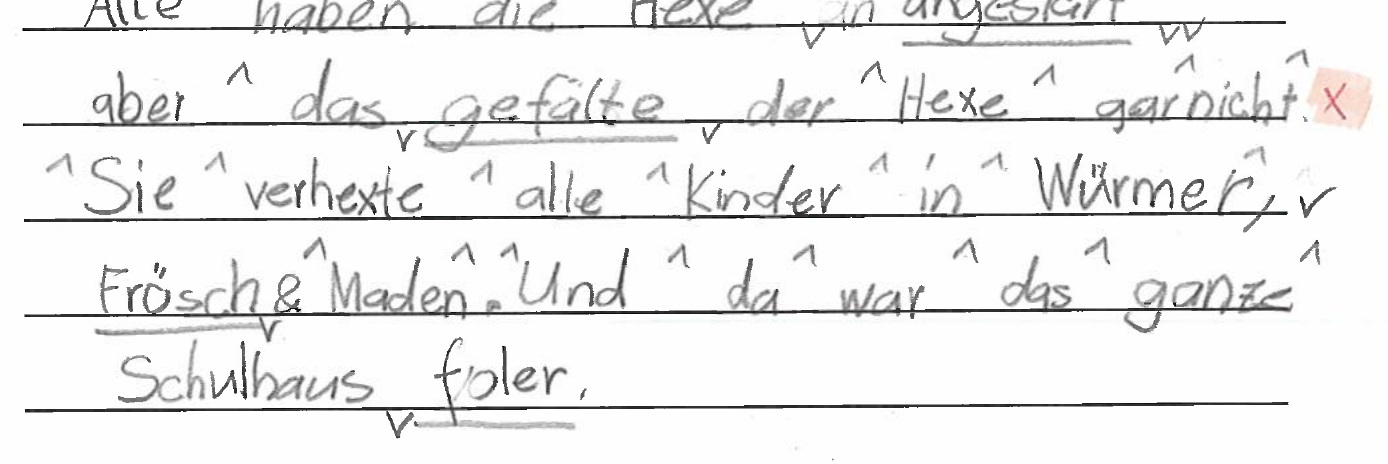
\includegraphics[width=0.90\linewidth]{images/pdf_optimized/ch6_children_3B_19_2-3_crop.jpg}
  \caption{Selected Children Handwritten sample detail cropped for readability. The example illustrates OCR-noise recovery discussed in the second qualitative paragraph: The local handwritten detail around the \texttt{\&} token is visible in the image and is consistent with the additional structure recovery in the reported M5 setup beyond OCR-conditioned text alone.}
  \label{fig:exp_qualitative_input_children}
\end{figure}

\paragraph{Why IAM is already easy for OCR-grounded methods.}
IAM shows the absence of measurable headroom. Sample \texttt{p06-042} is a plateau case rather than an M5-specific gain case: M3/\GPTFiveMarchShort{}, M4/\GPTFiveMarchShort{}, M5/\GPTFiveShort{}, and NNTP/NNTP all reach \(\LANormCombinedToken=\LineFOneNormToken=1.000\) with \(\CERNormToken=0.000\). That is precisely why it belongs in the qualitative analysis. It shows that some cleaner modern handwritten subsets are already almost solved once OCR line order is close to the ground truth, so richer image evidence does not necessarily create a new advantage; instead, it confirms a structure that is already largely recoverable from OCR-conditioned inputs.

\paragraph{Bullinger high-F1 positional failure.}
Bullinger supplies the sharpest positional rather than lexical failure. Sample 12517, summarized in the third row of Table~\ref{tab:exp_linebreak_comparison} and excerpted in Appendix Table~\ref{tab:app_qualitative_excerpt_blocks}, is the clearest high-\LineFOneNorm{} / low-\LANormCombined{} case already used in the qualitative table. The selected M1/\GPTFiveMarchShort{} row drops the opening line \texttt{234}, which is enough to force \(\LANormCombinedToken=0.000\) even though \(\LineFOneNormToken=0.909\), with \(\CERNormToken=0.006\). The matched M5/\GPTFiveShort{} row reaches \(\LANormCombinedToken=\LineFOneNormToken=1.000\) and \(\CERNormToken=0.000\). Many line strings survive as exact normalized strings, but the sequence-level alignment fails completely after the opening omission.

\paragraph{A boundary case for M5 interpretation.}
The final case bounds the M5 interpretation from the other direction by showing a page where an earlier LLM/VLM-based configuration is stronger. The fifth row of Table~\ref{tab:exp_linebreak_comparison}, expanded in Appendix Table~\ref{tab:app_qualitative_excerpt_blocks}, shows this directly for Washington sample 270: M3/\GPTFiveMarchShort{} reaches \(\LANormCombinedToken=\LineFOneNormToken=0.935\) with \(\CERNormToken=0.002\), while the selected M5/\QwenThirtyTwoShort{} row drops to \(0.871\) on both line metrics with the same \(\CERNormToken=0.002\). The M5 trace records \texttt{fallback\_projection} after \texttt{initial+repair}; the stored prediction locally over-splits the hyphenated \texttt{Recrui-\textbackslash nting} boundary as \texttt{Recrui\textbackslash n- ting}. The same sample is also the clearest NNTP-favored case against the matched Washington M5 row: The Washington NNTP fold prediction preserves the ground-truth split and reaches \(\LANormCombinedToken=\LineFOneNormToken=1.000\) with \(\CERNormToken=0.000\). Including this boundary case keeps the qualitative analysis aligned with the aggregate result: It illustrates trace and error patterns without turning an individual sample into the full RQ3 answer.

\FloatBarrier

\section{Interpretation and Validity Boundaries}
\label{sec:experimentation_analysis}

\paragraph{Supported interpretation.}
The clearest empirical pattern comes from reading the main handwritten overview together with the controlled LLM/VLM-based checks. M5 has the highest reported macro score among the evaluated LLM/VLM-based alignment setups in the overview table, and it remains highest wherever the exact-model comparison is complete. At the same time, the intermediate steps are not monotonic: M3 can already perform strongly on cleaner or OCR-friendly material, and M4 does not uniformly improve over M3. The supported conclusion is therefore about the reported evidence-and-control mix, with M5 interpreted as the evaluated context-rich line-image setup rather than as a universal stepwise ladder from M1 to M5.

\paragraph{Validity-boundary synthesis.}
The main boundaries are consolidated in Table~\ref{tab:exp_validity_boundaries}. They define the level at which the result tables should be read and preserve the chapter's main result: The reported evidence is most secure at the level of evaluated alignment setups, not isolated components.

\begin{table}[!htbp]
  \centering
  \caption{Compact interpretation boundaries for the Chapter~\ref{cha:experimentation} result layers. The table summarizes how dataset staging, provider provenance, output control, NNTP preprocessing, and sample-set availability bound the reported comparisons.}
  \label{tab:exp_validity_boundaries}
  \scriptsize
  \renewcommand{\arraystretch}{1.12}
  \setlength{\tabcolsep}{2.5pt}
  \begin{tabularx}{\linewidth}{@{}>{\raggedright\arraybackslash}p{0.20\linewidth}>{\raggedright\arraybackslash}p{0.31\linewidth}X@{}}
    \toprule
    \textbf{Boundary} & \textbf{Affects} & \textbf{Consequence for interpretation} \\
    \midrule
    Known-count staging for M4/M5 & Structured rows in Tables~\ref{tab:exp_handwritten_main_overview}, \ref{tab:exp_handwritten_controlled_model}, \ref{tab:exp_line_count_drift}, and \ref{tab:exp_method_weakness_mechanisms}; comparability summaries in Tables~\ref{tab:method_comparability_matrix} and \ref{tab:app_method_comparability_matrix_full}. & M4 and M5 test boundary assignment under known-count staging: The handwritten \texttt{ocr\_lines} cardinality matches the ground-truth line count. They are not blind page-side line-count or segmentation systems. \\
    \addlinespace[0.35em]
    Mixed line-crop provenance & M5 and NNTP rows in Tables~\ref{tab:exp_handwritten_main_overview}, \ref{tab:exp_best_vs_nntp}, \ref{tab:exp_bullinger_contextual}, and \ref{tab:exp_linebreak_comparison}. & Children Handwritten and IAM use dataset-provided line images, Bullinger uses PAGE/XML-derived crops, and Washington uses curated Kraken crops. The comparison is among evaluated configurations with their respective anchors, not among crop-generation pipelines. \\
    \addlinespace[0.35em]
    Model-configuration dependence & Overview and provenance tables: Tables~\ref{tab:exp_handwritten_main_overview}, \ref{tab:exp_handwritten_prompt_matrix}, \ref{tab:app_handwritten_prompt_provenance}, and \ref{tab:app_handwritten_prompt_detail_metrics}; controlled checks in Tables~\ref{tab:exp_handwritten_controlled_model} and \ref{tab:app_mistral_fixed_provider_matrix}. & The overview may use different model configurations across cells. M5 remains the highest-scoring row in the reported overview and in the exact-model OpenAI control, while intermediate M1--M4 rankings remain model- and dataset-sensitive. \\
    \addlinespace[0.35em]
    Projection versus raw returned text & M1--M5 comparisons in Tables~\ref{tab:exp_handwritten_main_overview} and \ref{tab:exp_handwritten_controlled_model}; line-count drift in Table~\ref{tab:exp_line_count_drift}; M5 traces in Table~\ref{tab:app_m5_trace_event_counts}; mechanisms in Table~\ref{tab:exp_method_weakness_mechanisms}. & M1--M3 score raw returned text, whereas M4/M5 may validate, repair, recover, fall back, and project a boundary plan onto the supplied transcription. This improves fixed-transcription validity but does not isolate projection, repair, fallback, or JSON validity as separate causes. \\
    \addlinespace[0.35em]
    Heuristic multi-page chunking for M1/M2 & Raw page-image regimes in Tables~\ref{tab:exp_handwritten_main_overview}, \ref{tab:exp_handwritten_controlled_model}, and \ref{tab:exp_method_weakness_mechanisms}. & The affected handwritten samples are multi-page Bullinger cases: 31/162 overall and 31/59 within Bullinger. M1/M2 results are evidence about the implemented chunked configurations, not isolated page-image or OCR/HTR hint effects. \\
    \addlinespace[0.35em]
    NNTP symbol-inventory preprocessing & NNTP rows in Tables~\ref{tab:exp_best_vs_nntp}, \ref{tab:exp_bullinger_contextual}, and \ref{tab:exp_linebreak_comparison}; audit summary in Table~\ref{tab:app_nntp_symbol_filter_audit}. & NNTP applies symbol-inventory preprocessing before alignment. The shared line-metric comparison remains useful; character-level comparisons against M1--M5 need this preprocessing caveat. \\
    \addlinespace[0.35em]
    Sample-set mismatch and small samples & NNTP comparison tables, especially Tables~\ref{tab:exp_best_vs_nntp} and \ref{tab:exp_bullinger_contextual}; cross-dataset readings of Tables~\ref{tab:exp_handwritten_main_overview} and \ref{tab:exp_handwritten_controlled_model}. & Children and Washington use NNTP cross-validation macro summaries, IAM uses a legacy single run, Bullinger lacks a thesis-side matched full-sample NNTP row, and IAM/Washington each have \(n=20\). The M5--NNTP result is close and dataset-dependent rather than one homogeneous winner. \\
    \addlinespace[0.35em]
    Missing deterministic scaffold baselines & Causal readings of Tables~\ref{tab:exp_handwritten_main_overview}, \ref{tab:exp_handwritten_controlled_model}, \ref{tab:exp_line_count_drift}, \ref{tab:app_m5_trace_event_counts}, and \ref{tab:exp_method_weakness_mechanisms}. & The result set does not include full-sample deterministic controls such as OCR-line dynamic alignment, known-\(N\) proportional splitting, OCR-only projection, or no-projection M4/M5 ablations. The observed gains belong to reported configurations rather than to isolated scaffold components. \\
    \bottomrule
  \end{tabularx}
\end{table}

\FloatBarrier

\paragraph{Chapter summary.}
\label{sec:experimentation_summary}

Taken together, the experiments support a comparison of reported alignment setups with different evidence and output control rather than isolated components. M5 has the highest reported macro score among the evaluated LLM/VLM-based handwritten alignment setups, and the controlled checks preserve this main result wherever complete comparisons exist. The printed rows add limited M1--M3 modality context, while the NNTP comparison shows that deterministic forced alignment remains a competitive reference point. The result is therefore an evidence base for newline-only transcription alignment under increasingly structured evidence and output control, with the main interpretation boundaries summarized in Table~\ref{tab:exp_validity_boundaries}.

% Chapter 7 concludes the thesis.
% Content: summary of findings about LLM/VLM line alignment performance, answers to the research
% questions, key limitations, and concrete directions for future work.

\chapter{Conclusion}
\label{cha:conclusion}

Newline-only transcription alignment is more than a formatting problem: It is a controlled way to test how well systems recover line structure when the transcription itself is fixed. By preserving the non-newline character sequence, the evaluation separates boundary recovery from OCR/HTR recognition and makes different alignment setups comparable under one target. Within the handwritten scope, the context-rich M5 setup has the highest reported macro score among the evaluated LLM/VLM configurations, while NNTP remains a close deterministic reference on the matched datasets. The thesis therefore contributes a task definition, an evaluation protocol, a documented benchmark, and practical evidence about the role of structured output control.

\section{Contribution and Completed Work}
\label{sec:conclusion_summary}

This thesis addressed newline-only alignment as defined in \autoref{sec:theory_problem_definition} and instantiated as a shared evaluation target in \autoref{sec:method_common_contract}. In operational terms, the task is to recover line boundaries for supplied transcriptions while preserving character identity and order exactly. That separation is the central methodological contribution: Boundary recovery is evaluated as layout reconstruction behavior, not as generic text generation quality.

The implementation contribution is a six-way comparison against that shared target, with M1--M5 as LLM/VLM-based methods and NNTP as the deterministic forced-alignment baseline. NNTP is used in that role because it aligns a fixed transcription to recognizer-derived line evidence instead of freely generating a new transcription, following the forced-alignment family discussed in \autoref{sec:sota_deterministic_baselines}. Around this comparison, the project also implemented the \OCRHTR pipeline, line-image preparation, resumable evaluation workflows, and artifact packaging that keeps the comparison inspectable beyond isolated examples; the reproducibility registry is kept in Appendix~\ref{cha:appendix_audit}.

The empirical focus of the thesis is a handwritten comparison layer over Bullinger Handwritten, Children Handwritten, IAM Handwritten as a fixed 20-form IAM subset, and Washington Handwritten. Within that scope, all reported dataset scores are macro-averages over sample IDs, and reporting prioritizes \LANormForward{} and \LANormReverse{} together with their combined normalized view \LANormCombined, while \LineFOneNorm, \CERNorm, and \WERNorm remain complementary diagnostics rather than primary indicators; \autoref{sec:experimentation_protocol} defines this reporting protocol, including the Levenshtein-based CER/WER diagnostics \thesiscite{levenshtein1966binaryCodes}.

\section{Answers to the Research Questions}
\label{sec:conclusion_rq_answers}

\begin{table}[H]
  \centering
  \caption{Compact answers to the three research questions. The detailed prose below expands the evidence and caveats behind each row.}
  \label{tab:conclusion_rq_compact_answers}
  \footnotesize
  \setlength{\tabcolsep}{3pt}
  \renewcommand{\arraystretch}{1.12}
  \begin{tabularx}{\linewidth}{@{}>{\raggedright\arraybackslash}p{0.12\linewidth}>{\raggedright\arraybackslash}p{0.28\linewidth}>{\raggedright\arraybackslash}p{0.31\linewidth}Y@{}}
    \toprule
    \textbf{Research question} & \textbf{Short answer} & \textbf{Main evidence} & \textbf{Main limitation} \\
    \midrule
    RQ1 & M5 in the context-rich structured setup has the highest reported macro score among evaluated LLM/VLM handwritten configurations. & Descriptive overview of evaluated setups, method overview, and complete exact-model control where available (\autoref{fig:exp_handwritten_llm_model_overview}; \autoref{tab:exp_handwritten_main_overview}; \autoref{tab:exp_handwritten_controlled_model}). & Intermediate steps are non-monotonic; method availability is unequal; component-level attribution remains bounded. \\
    RQ2 & M5 and NNTP are close/tie-dominated on the matched handwritten comparison sets. & Matched dataset-level table and paired win/tie/loss counts (\autoref{tab:exp_best_vs_nntp}). & Differences are dataset-dependent; Bullinger is handled through a published-baseline subset comparison, with Subset~1 direct and Subset~2 contextual; NNTP retains the preprocessing caveat. \\
    RQ3 & Structured output control, repair, fallback, and projection make LLM/VLM outputs compatible with the fixed-transcription requirement. & Structured output-validity analysis and event-count audit (\autoref{sec:experimentation_output_control_audit}; \autoref{tab:app_m5_trace_event_counts}). & Evidence supports the structured setup rather than isolated components separated from evidence, staging, and provider effects. \\
    \bottomrule
  \end{tabularx}
\end{table}

Line-level correspondence also gives the result a Digital Humanities value beyond the score tables. For collections where a transcription already exists, newline-only alignment can connect that trusted text back to local line positions without asking a system to rewrite the scholarly transcription. That makes the output useful for inspection, training-data preparation, and local error analysis, because analysts can compare a text span, its proposed line boundary, and the relevant image evidence under one fixed character sequence. The same constraint also bounds the contribution: This task does not replace scholarly transcription, and it does not solve blind page segmentation or line-count inference from images alone \thesiscite{DriscollLevelsTranscription,Muehlberger2019TransformingScholarship,vidal2023pageLevelAssessment}.

Because the contribution is methodological as well as empirical, the conclusions are framed by the available evidence and its controls. Table~\ref{tab:conclusion_rq_compact_answers} gives the compact answer layer; the following subsections unpack the supporting evidence and limits for each research question.

\subsection{RQ1: Which input-evidence configurations most improve newline-boundary accuracy for fixed transcriptions?}
\label{sec:conclusion_rq1}

RQ1 gives the main LLM/VLM-side finding: Across the handwritten comparison, M5 has the highest reported macro score among evaluated LLM/VLM-based setups on all four datasets in the provider-mixed descriptive overview, and the controlled LLM/VLM-based checks support the same result wherever the evaluation records contain a complete five-method comparison (\autoref{fig:exp_handwritten_llm_model_overview}; \autoref{tab:exp_handwritten_main_overview}; \autoref{tab:exp_handwritten_controlled_model}). This makes the context-rich structured setup the clearest positive result of the LLM/VLM experiments. The supported reading remains configuration-level: M5 combines ordered line-image context, OCR/HTR line text, page context, structured line metadata, validation, fallback, and projection. The evidence therefore supports M5 as the highest-scoring evaluated LLM/VLM-based setup, not a monotonic M1--M5 ladder or an isolated causal estimate for line-image evidence alone.

\subsection{RQ2: How does the highest-scoring reported LLM/VLM-based regime compare with NNTP, a deterministic forced-alignment baseline, under the same newline-only evaluation target?}
\label{sec:conclusion_rq2}

RQ2 places that M5 result beside a deterministic aligner, and the supported reading is close and tie-dominated rather than one-sided. The matched set is Children Handwritten, IAM Handwritten, and Washington Handwritten. Bullinger is handled separately through the published Bullinger baseline: Subset~1 supports a direct subset-level comparison, while Subset~2 remains contextual because the inventories differ. Within that matched set, Children slightly favors M5, IAM is tied, and Washington slightly favors NNTP; paired counts from available prediction texts reinforce the close reading with 4 LLM/VLM wins, 2 NNTP wins, and 57 ties on Children, 20 ties on IAM, and 2 LLM/VLM wins, 4 NNTP wins, and 14 ties on Washington (\autoref{tab:exp_best_vs_nntp}). The comparison is useful precisely because both regimes are strong in different ways: M5 is a structured VLM regime whose generated response is checked, repaired, or projected, whereas NNTP is a fixed-transcription forced aligner over recognizer evidence. Character-level interpretations keep the NNTP preprocessing boundary explicit for both the matched rows and the Bullinger-specific comparison \thesiscite{peer2025ctcBullingerAlignment}.

\subsection{RQ3: To what extent do structured output control, repair, fallback, and projection make LLM/VLM outputs valid under the fixed-transcription newline-only requirement?}
\label{sec:conclusion_rq3}

RQ3 explains why output form is central to the fixed-transcription task. Raw-output LLM/VLM methods can request newline-only behavior, but they do not guarantee preservation of the fixed non-newline character sequence. The structured methods add line-count checks, repair attempts, fallback behavior, and projection to the supplied transcription, making the final scored outputs compatible with the fixed-transcription requirement rather than merely prompt-compliant.

The RQ3 claim is therefore about the structured evaluated setup. Validation, repair, fallback, and projection turn malformed or character-drifting generations into inspectable boundary plans or reject them through fallback paths. The available records keep those controls coupled with known-count staging, crop provenance, provider choice, and richer input evidence, so isolated effects of repair, fallback, or projection remain future ablation questions.

\section{Limits of the Current Evidence}
\label{sec:conclusion_limits}

Chapter~\ref{cha:experimentation} gives the detailed validity account, especially in Table~\ref{tab:exp_validity_boundaries}. The limits summarized here are therefore not separate weaknesses of the task formulation, but the boundaries within which the research-question answers should be read. The strongest claims are claims about evaluated alignment setups. Evidence inputs, prompt and output format, validation, repair, fallback, projection, provider or model behavior, and line-image preparation are bundled in the reported configurations. The results therefore compare practical alignment setups rather than isolating the contribution of any single component.

\paragraph{Staging, data, and reproducibility.}
M4 and M5 use known-count structured staging in the evaluated handwritten setup: The stored ordered line metadata supplies a line count that matches the ground truth. These rows therefore test boundary assignment when an ordered line inventory is available, not blind line-count inference from a page image alone. The line-image sources also differ across datasets. Children Handwritten and IAM use dataset-provided line images, Bullinger uses PAGE/XML-derived crops, and Washington uses curated Kraken crops. Reproducibility is strongest for the public or fully disclosed parts of the pipeline; for Children Handwritten, external reproduction depends on access to the controlled AIBEX source export.

\paragraph{Compared outputs and baselines.}
The LLM/VLM overview is descriptive and provider-mixed, so it supports the reported M5 result rather than a provider-stable model ranking. The scored outputs also differ by method family: M1--M3 score raw returned model strings, whereas M4 and M5 may validate, repair, recover, fall back, and project a boundary plan onto the supplied transcription before scoring. NNTP remains a strong deterministic comparator at the shared line-metric level, while its PyLaia symbol-inventory preprocessing should be kept in mind for character-level interpretations.

Bullinger contributes to the NNTP comparison through the published Bullinger baseline rather than through a new thesis-side full-\(59\)-sample NNTP run. This is still useful evidence. Subset~1 gives a direct subset-level comparison because the thesis subset matches the published inventory at the letter and line level. Subset~2 remains contextual because the thesis and paper inventories differ. For this reason, the sample-level tie-dominance claim is restricted to Children, IAM, and Washington, while Bullinger is used as an external published-baseline check.

\paragraph{Missing evaluation layers.}
The thesis does not include deterministic scaffold baselines, no-projection ablations, cost/runtime analysis, or human-in-the-loop correction studies. These are natural next steps rather than prerequisites for the present contribution. Within the current scope, the evidence supports three main conclusions: M5 has the highest reported macro score among the evaluated LLM/VLM-based handwritten setups; M5 and NNTP are close on the same-sample handwritten comparison sets; and structured output control is important for fixed-transcription validity. These boundaries make the contribution clearer: Newline-only alignment is a practical benchmark for comparing alignment setups today, and a basis for more component-level and operational evaluations in future work.

\section{Future Work}
\label{sec:conclusion_future_work}

The most important next steps are those that keep the newline-only constraint central rather than treating it as a by-product of general OCR, HTR, or document-understanding systems. Three directions follow most directly from the results of this thesis.

\paragraph{Dedicated newline-boundary prediction.}
A first direction is to train a model specifically for newline-only alignment rather than relying on a general-purpose LLM or VLM to produce a corrected copy of the transcription. Such a model could represent the supplied transcription as a character or token sequence, combine it with visual page evidence, OCR/HTR hints, and ordered line context, and predict a boundary vector over the admissible insertion positions. This would move the problem from prompting toward a dedicated boundary predictor whose output space matches \(\mathcal{Y}(x)\) from \autoref{sec:theory_problem_definition}. It would also make it easier to test which signals are useful under a single trained objective, for example through ablations of line-count access, OCR scaffolding, image crops, and projection \thesiscite{likformansulem2006textLineSurvey,huang2022layoutlmv3,li2023trocr}.

\paragraph{Constrained decoding and boundary search.}
A second direction is to develop decoding or search methods that guarantee exact preservation of the fixed transcription while optimizing boundary placement. Rather than generating text first and projecting a usable line plan afterward, a decoder could operate directly over boundary vectors, dynamic-programming states, finite-state constraints, or token masks that admit only newline insertions between existing characters. This would connect the thesis task to constrained decoding and forced-alignment research while keeping the target explicit: The output should be a scored boundary plan, not a free string that later happens to be repairable \thesiscite{geng2023grammar,hokamp2017gridBeam,post2018fast,fischer2011icdarInaccurateAlignment,peer2025ctcBullingerAlignment}.

\paragraph{Human-in-the-loop scholarly correction.}
A third direction is an interactive correction workflow for scholarly transcription environments. Such a system could highlight uncertain newline-boundary decisions, show the relevant page crop, OCR/HTR line hint, neighboring text span, and alternative boundary plans, and let human experts approve or correct the proposed alignment. The research question would not only be whether automatic scores improve, but also how much expert time is saved, which uncertainty signals are interpretable, and how corrected decisions should be stored so that later editions can distinguish machine suggestions from scholarly approval. This direction connects the technical boundary-recovery task back to the Digital Humanities setting in which line structure supports inspection, citation, training data preparation, and editorial work \thesiscite{DriscollLevelsTranscription,Muehlberger2019TransformingScholarship,vidal2023pageLevelAssessment}.

\section{Final Remarks}
\label{sec:conclusion_final_remarks}

This thesis establishes newline-only transcription alignment as a focused document-analysis task: Recover line boundaries while preserving the supplied transcription. The experiments show that structured LLM/VLM setups can be effective under this constraint, especially when line-image evidence is combined with validation and projection, but they also show that deterministic forced alignment remains a strong reference point. The contribution is a controlled task formulation, a documented benchmark, and a reproducible basis for future work on dedicated boundary prediction, constrained decoding, and human-in-the-loop scholarly correction.

\cleardoublepage
\chapter*{Use of AI Tools}

AI-based tools were used as assistive tools during the preparation of this thesis. ChatGPT supported drafting, language refinement, and structural review. Codex supported code-related work, LaTeX editing, and consistency checks within the thesis project. DeepL supported translation of selected passages. Perplexity supported preliminary literature exploration and the identification of potentially relevant sources. Outputs from these tools were treated as suggestions, not as authoritative sources. Claims, citations, dataset descriptions, experimental results, code changes, and final wording were checked against the LaTeX project, the source code repository, the experimental result files, and the cited literature. The author remains responsible for the content, interpretation, results, and conclusions of the thesis.


\begingroup
\sloppy
\cleardoublepage
\phantomsection
\addcontentsline{toc}{chapter}{\bibname}
\bibliography{thesis}
\endgroup
\bibliographystyle{plainnat}

\appendix
% Supplementary appendix material for structured-method auditability and supporting tables.

\chapter{Supplementary Method and Evaluation Details}
\label{cha:appendix_audit}

\section{Prompt Templates and Raw-Output LLM/VLM Regimes}
\label{sec:appendix_prompt_templates}

Chapter~\ref{cha:method} gives the thesis-level prompt requirements needed to understand the evaluated regimes directly in the main text. This appendix keeps the corresponding reproducibility registry. Table~\ref{tab:app_prompt_template_registry} preserves the archived implementation identifiers, run-configuration details, and companion-repository paths for the retained prompt family so that the reported handwritten rows can be traced back to concrete implementation artifacts. The registry does not imply provider-independent reproducibility, because backend behavior, image-budget handling, and unlogged provider-side settings still affect the realized requests and responses.

\begin{table}[H]
  \centering
  \caption{Prompt-template reproducibility registry for the retained prompt family. Exact constants and companion-repository paths are preserved because they anchor the archived implementation identifiers discussed in Chapter~\ref{cha:method}.}
  \label{tab:app_prompt_template_registry}
  \footnotesize
  \renewcommand{\arraystretch}{1.08}
  \setlength{\tabcolsep}{4pt}
  \begin{tabularx}{\linewidth}{@{}>{\raggedright\arraybackslash}p{0.07\linewidth}>{\raggedright\arraybackslash}p{0.19\linewidth}>{\raggedright\arraybackslash}p{0.28\linewidth}Y@{}}
    \toprule
    \textbf{Method} & \textbf{Thesis-level prompt name} & \textbf{Archived implementation identifier(s) and run-configuration detail} & \textbf{Companion-repository path / note} \\
    \midrule
    M1 & M1 image-transcription prompt & \path{PROMPT_TEMPLATE_M1}; no retained prompt-variant override & prompt source: \path{utils/prompts.py}; evaluation entry point: \path{jobs/eval/m1/common_m1_eval.sbatch} \\
    M2 & M2 image-transcription-\OCRHTR prompt & \path{PROMPT_TEMPLATE_M2}; no retained prompt-variant override & prompt source: \path{utils/prompts.py}; evaluation entry point: \path{jobs/eval/m2/common_m2_eval.sbatch} \\
    M3 & M3 transcription-\OCRHTR prompt & \path{PROMPT_TEMPLATE_M3}; no retained prompt-variant override & prompt source: \path{utils/prompts.py}; evaluation entry point: \path{jobs/eval/m3/common_m3_eval.sbatch} \\
    M4 & M4 structured OCR-line prompt; M4 repair prompt & \path{PROMPT_TEMPLATE_M4_BASELINE}; \path{M4_REPAIR_PROMPT_TEMPLATE}; run-configuration detail \path{PROMPT_VARIANT=baseline} & prompt source: \path{utils/prompts.py}; evaluation entry point: \path{jobs/eval/m4/common_m4_eval.sbatch} \\
    M5 & retained context-rich M5 boundary-context prompt; M5 repair prompt & \path{PROMPT_TEMPLATE_M5_BOUNDARY_CONTEXT_V2}; \path{M5_REPAIR_PROMPT_TEMPLATE}; run-configuration detail \path{PROMPT_VARIANT=boundary_context_v2} for the \contextHundred{} rows & prompt source: \path{utils/prompts.py}; evaluation entry point: \path{jobs/eval/m5/common_m5_eval.sbatch}; see note for archived handwritten batch files \\
    \bottomrule
  \end{tabularx}
  \vspace{0.35em}

  \parbox{0.96\linewidth}{\footnotesize\raggedright \textit{Note.} Exact constants and companion-repository paths are preserved verbatim because this table functions as a reproducibility registry rather than as a conceptual method summary. For M1--M3, few-shot examples are injected only through the method-specific formatter when \(n\)\nobreakdash-shot \(>0\). The limited 1-shot pilot in \autoref{sec:experimentation_one_shot_exploratory} is historical diagnostic evidence only and does not alter the retained prompt-family registry or the main M1--M5 maxima. For reproducibility, the one-example prompt used deterministic same-dataset example selection with random seed 42. The Washington runs were stored under the earlier internal \texttt{easy\_historical} label and are reported in the thesis as Washington Handwritten. For M4, the boundary-anchored alternative remains present in code but is not the retained default configuration. For M5, the archived handwritten batch files are \path{jobs/eval/m5/bullinger_handwritten_context100_0shot.sbatch}, \path{jobs/eval/m5/children_handwritten_context100_0shot.sbatch}, \path{jobs/eval/m5/washington_handwritten_context100_0shot.sbatch}, and \path{jobs/eval/m5/iam_handwritten_rep20_context100_0shot.sbatch}; the companion orchestration path is \path{jobs/orchestrators/eval_handwritten_m5_context100_api_models.sbatch}. Judge templates exist in code, but the retained recipe disables candidate judging.}
\end{table}

\subsection{Task-Critical Prompt Excerpts}
\label{sec:appendix_prompt_excerpts}

The following excerpts preserve the task-critical wording from the retained templates while omitting repeated headings, few-shot material, and long per-sample payloads. The evaluation runners fill the placeholders for the transcription, OCR/HTR text, expected line count, ordered line hints, and line-image manifest. M4 and M5 use the literal instruction that the transcription is the only source of characters; M1--M3 express the same constraint through the correct-transcription, exact-wording, and no-character-alteration instructions quoted below. M1--M3 use raw text prompts and are evaluated directly; M4 and M5 use strict JSON templates, repair prompts, and projection before scoring. There is no separate M5 recovery prompt constant in the retained code: loose recovery is implemented in the runner, while structural and quality repair calls reuse \path{M5_REPAIR_PROMPT_TEMPLATE} with generated error messages. Candidate-judge prompt constants are present in code, but the retained \contextHundred{} recipe disables judging.

\paragraph{\texttt{PROMPT\_TEMPLATE\_M1}.}
\begin{lstlisting}[basicstyle=\scriptsize\ttfamily,breaklines=true,columns=fullflexible]
# Role and Objective
Process a scanned page image and its transcription (continuous text; no line breaks) to reconstruct line breaks that match the page's visual line layout.

# Instructions
- Locate the exact wording for each visible line within the transcription.
- Insert newline characters at precise locations matching the visual end of each line in the image.
- Do not add, remove, or alter any characters other than adding newlines.
- Output only the visible text from the provided page, segmented precisely by these line breaks.
- Ignore image lines that do not have an exact transcriptional match.

Transcription:
{transcription}
\end{lstlisting}

\paragraph{\texttt{PROMPT\_TEMPLATE\_M2}.}
\begin{lstlisting}[basicstyle=\scriptsize\ttfamily,breaklines=true,columns=fullflexible]
# Role and Objective
Align the correct transcription of a scanned page to match the visual line structure, using the page image as the primary reference and HTR/OCR output as a structural guide.

# Instructions
- Use the page image as the main reference for true visual line breaks.
- Use the HTR/OCR output to help identify line boundaries, especially where the image is ambiguous.
- Insert newline characters into the correct transcription at positions matching visual line ends.
- Do not add, remove, or alter any characters other than adding newlines.
- Each visual line in the image should correspond to one line in your output.

Correct transcription:
{transcription}

HTR/OCR output with line breaks:
{htr}
\end{lstlisting}

\paragraph{\texttt{PROMPT\_TEMPLATE\_M3}.}
\begin{lstlisting}[basicstyle=\scriptsize\ttfamily,breaklines=true,columns=fullflexible]
# Role and Objective
Align a correct transcription (no line breaks) to match the line structure indicated by an HTR/OCR output (which has line breaks but may contain character errors).

# Instructions
- Use the HTR/OCR output to determine where line breaks should be inserted in the correct transcription.
- Do not add, remove, or alter any characters in the transcription other than inserting newlines.
- Handle HTR/OCR character errors by finding the best alignment between corresponding text segments.
- Each line in the HTR/OCR should correspond to one line in your output.

Correct transcription:
{transcription}

HTR/OCR output with line breaks:
{htr}
\end{lstlisting}

\paragraph{\texttt{PROMPT\_TEMPLATE\_M4\_BASELINE}.}
\begin{lstlisting}[basicstyle=\scriptsize\ttfamily,breaklines=true,columns=fullflexible]
# Role and Objective
Align a correct transcription (no line breaks) to an ordered list of PyLaia line hypotheses.

# Instructions
- The transcription is the only source of characters.
- The PyLaia line hypotheses are structural hints only; they may contain OCR errors.
- Produce exactly {num_lines} output lines in reading order.
- Do not add, remove, or alter transcription characters.
- Do not copy page or line metadata into the output.
- The concatenation of your output lines must exactly equal the transcription.

# Output Format
Return strict JSON only, with no code fences or extra text:
{"lines": ["...", "..."]}

Correct transcription:
{transcription}

Ordered PyLaia line hypotheses ({num_lines} lines):
{line_hints}
\end{lstlisting}

\paragraph{\texttt{M4\_REPAIR\_PROMPT\_TEMPLATE}.}
\begin{lstlisting}[basicstyle=\scriptsize\ttfamily,breaklines=true,columns=fullflexible]
Your previous response was invalid.
Error: {error_message}

Follow these rules:
{instruction_block}
- Return only strict JSON with exactly {num_lines} strings in the "lines" array.

Correct transcription:
{transcription}

Ordered PyLaia line hypotheses ({num_lines} lines):
{line_hints}

Previous invalid response:
{previous_response}
\end{lstlisting}

\paragraph{\texttt{PROMPT\_TEMPLATE\_M5\_BOUNDARY\_CONTEXT\_V2}.}
\begin{lstlisting}[basicstyle=\scriptsize\ttfamily,breaklines=true,columns=fullflexible]
# Role and Objective
Align a correct transcription (no line breaks) to an ordered set of line images.

# Instructions
- The transcription is the only source of characters.
- Use the supplied line-level images as the primary anchors for line boundaries.
- Produce exactly {num_lines} output lines in the same reading order as the supplied line images.
- Treat line image i as the hard local anchor for output line i.
- Keep uncertainty local: if one line is ambiguous, do not absorb text from its neighbors unless the images clearly require it.
- Preserve short, odd, or fragmentary standalone lines when the images suggest them, including page numbers, dates, headings, salutations, symbols, addresses, and brief tail fragments.
- If a line image appears much shorter than its neighbors, prefer assigning it a shorter transcription span instead of smoothing the boundary away.
- Use the global page context only to prevent long-range drift, not to override a clear local line image anchor.
- When uncertain between two nearby split points, prefer the earlier split that avoids pushing text into later lines.
- Do not leave the first or last output line empty unless the corresponding line image is genuinely blank.
- Do not add, remove, or alter transcription characters.
- Do not copy metadata into the output.
- The concatenation of your output lines must exactly equal the transcription.
- You will receive one or more numbered strip images. Each strip contains consecutive line crops in reading order, separated by black bars, and each row is labeled with its output line number in the left gutter.
- If full page images are provided, use them only as global layout context for indentation, relative line length, page transitions, and short header or signature blocks.
- If OCR line-text hints are provided below, use them only as a secondary structural hint. They may contain recognition errors.

# Output Format
Return strict JSON only, with no code fences or extra text:
{"lines": ["...", "..."]}

Correct transcription:
{transcription}

Ordered line-image manifest ({num_lines} lines):
{line_image_manifest}

Optional OCR line hints:
{ocr_text_section}
\end{lstlisting}

\paragraph{\texttt{M5\_REPAIR\_PROMPT\_TEMPLATE}.}
\begin{lstlisting}[basicstyle=\scriptsize\ttfamily,breaklines=true,columns=fullflexible]
Your previous response was invalid.
Error: {error_message}

Follow these rules:
{instruction_block}
- Return only strict JSON with exactly {num_lines} strings in the "lines" array.

Correct transcription:
{transcription}

Ordered line-image manifest ({num_lines} lines):
{line_image_manifest}
{ocr_text_section}

Previous invalid response:
{previous_response}
\end{lstlisting}

\paragraph{M5 recovery path.}
No separate recovery prompt is present for M5. After an invalid first response and invalid repair response, the retained runner first tries to parse loose JSON line arrays from the initial or repair response, scores them against OCR fallback hint lines when those hints are available, reconciles or merges them to the expected \texttt{\{num\_lines\}}, and projects the reconciled plan to the untouched transcription. If that recovery fails, it uses OCR hint lines or exact-count plain response lines as fallback boundary hints before projection; if no usable line hints remain, the runner raises an error rather than fabricating a final transcription.

\subsection{Raw-Output LLM/VLM Skeletons}
\label{sec:appendix_prompt_only_pseudocode}

The raw-output LLM/VLM regimes M1--M3 share one reproducibility-relevant property that is absent from M4 and M5: The first backend response is evaluated directly, without parser-backed repair or boundary projection afterward. The following skeletons supplement the main-text summaries and keep the generation loop explicit without any recovery stage.

\paragraph{M1.}
{\footnotesize
\begin{alltt}
Input: Ordered page images I_1..I_k,
       fixed transcription x, optional few-shot examples
1. load I_1..I_k and the untouched transcription x
2. if k > 1, split x heuristically into
   k contiguous word-respecting chunks
3. for each non-empty chunk i:
     Build the prompt with PROMPT_TEMPLATE_M1
     send (I_i, chunk_i) to the multimodal backend
4. concatenate the page responses in page order
5. evaluate the raw returned text directly
\end{alltt}
}

\paragraph{M2.}
{\footnotesize
\begin{alltt}
Input: Ordered page images I_1..I_k,
       fixed transcription x, OCR/HTR text h
1. load I_1..I_k, x, and the OCR/HTR hint text h
2. if k > 1, split x and h independently into
   k contiguous word-respecting chunks
3. for each non-empty page chunk i:
     Build the prompt with PROMPT_TEMPLATE_M2
     send (I_i, x_i, h_i) to the multimodal backend
4. concatenate the page responses in page order
5. evaluate the raw returned text directly
\end{alltt}
}

\paragraph{M3.}
{\footnotesize
\begin{alltt}
Input: Fixed transcription x,
       OCR/HTR text h, optional few-shot examples
1. load x and the OCR/HTR hint text h
2. build the prompt with PROMPT_TEMPLATE_M3
3. send (x, h) to the text backend in one call
4. store the raw returned text as the prediction
5. evaluate the raw returned text directly
\end{alltt}
}

\subsection{Expanded Comparability Matrix}
\label{sec:appendix_method_comparability}

Table~\ref{tab:app_method_comparability_matrix_full} expands the compact validity summary from Table~\ref{tab:method_comparability_matrix}. It keeps the fuller appendix-only registry form needed for interpretation: Evidence inputs, line-count source, output-control regime, projection or fallback behavior, provider dependence, and the NNTP symbol-filter caveat. The goal is readability for later appendix consultation rather than compactness for the main argument.

\begin{table}[p]
  \centering
  \caption{Expanded comparability matrix for the implemented handwritten regimes. The table keeps the appendix-only interpretation registry in one place: Evidence inputs, stored line-count provenance, output-control regime, projection or fallback behavior, provider dependence, and the NNTP PyLaia symbol-filter caveat.}
  \label{tab:app_method_comparability_matrix_full}
  \scriptsize
  \renewcommand{\arraystretch}{1.08}
  \setlength{\tabcolsep}{3pt}
  \begin{tabularx}{\linewidth}{@{}>{\raggedright\arraybackslash}p{0.07\linewidth}>{\raggedright\arraybackslash}p{0.15\linewidth}>{\raggedright\arraybackslash}p{0.12\linewidth}>{\raggedright\arraybackslash}p{0.13\linewidth}>{\raggedright\arraybackslash}p{0.08\linewidth}>{\raggedright\arraybackslash}p{0.10\linewidth}>{\raggedright\arraybackslash}p{0.11\linewidth}Y@{}}
    \toprule
    \textbf{Method} & \textbf{Evidence} & \textbf{Line-count source} & \textbf{Output control} & \textbf{Projection} & \textbf{Fallback} & \textbf{Provider dependence} & \textbf{Caveat} \\
    \midrule
    M1 & ordered page image(s) + fixed transcription & none; length emerges from raw backend output & prompt instructions only & no & none & high; raw multimodal output is scored directly & multi-page chunking is heuristic rather than ground-truth page aligned \\
    M2 & ordered page image(s) + OCR/HTR hint text + fixed transcription & none; length emerges from raw backend output & prompt instructions only & no & none & high; raw output and OCR-conditioned prompting both matter & inherits OCR noise and the same heuristic multi-page chunking as M1 \\
    M3 & OCR/HTR hint text + fixed transcription & none; length emerges from raw backend output & prompt instructions only & no & none & high; raw text output is scored directly & no visual evidence remains to correct OCR-side ordering or line-break mistakes \\
    M4 & ordered OCR lines + fixed transcription & stored \texttt{ocr\_lines} count; matches ground truth in the reported evaluation set & strict JSON, one repair prompt, parser validation & yes & deterministic OCR-line projection after failed repair & moderate; parser-side recovery reduces backend variation in the final string & count is not page-predicted and the scaffold inherits OCR quality \\
    M5 & ordered line crops + OCR/HTR line text + page images + fixed transcription in the evaluated configuration & stored \texttt{ocr\_lines} count; matches ground truth in the reported evaluation set & strict JSON, repair, recovery, structural and quality checks & yes & loose model-line recovery, otherwise deterministic projection & high; backend image budgets affect the realized prompt bundle & mixed crop provenance and stored count remain part of the regime \\
    NNTP & staged line images + recognizer output + fixed transcription & staged line-image set after dataset-specific preparation & deterministic forced alignment & no & not applicable & no API provider; recognizer and checkpoint still matter & labels are filtered to the active PyLaia symbol inventory before alignment \\
    \bottomrule
  \end{tabularx}
  \vspace{0.35em}

  \parbox{0.95\linewidth}{\footnotesize\raggedright \textit{Note.} The matrix stays in the appendix because it is interpretively important but too dense for the main text. It preserves the same variables used throughout the thesis to separate direct comparisons from contextual ones: Evidence, line-count provenance, output control, projection, fallback, provider dependence, and the NNTP symbol-filter caveat.}
\end{table}

\FloatBarrier

\section{Expanded Error-Mechanism Evidence}
\label{sec:appendix_method_weakness_evidence}

Table~\ref{tab:app_method_weakness_evidence} expands the compact weakness summary in Table~\ref{tab:exp_method_weakness_mechanisms}. It keeps the counts, named sample IDs, trace evidence, and longer mechanism explanations in the appendix so that the Chapter~\ref{cha:experimentation} discussion can remain readable without losing audit detail. Counts are row counts rather than sample-ID macro-averages, and metric examples or trace averages use whitespace-normalized values where \LANormCombined{}, \CERNorm{}, or \WERNorm{} is named.

\begin{landscape}
\begin{table}[p]
  \centering
  \caption{Expanded evidence behind the method weakness and mechanism summary in Table~\ref{tab:exp_method_weakness_mechanisms}. Counts summarize auditable rows in the documented prediction- and trace-level analysis; named samples are illustrative cases only. For NNTP, character-level interpretation preserves the preprocessing caveat.}
  \label{tab:app_method_weakness_evidence}
  \scriptsize
  \renewcommand{\arraystretch}{1.10}
  \setlength{\tabcolsep}{4pt}
  \begin{tabularx}{\linewidth}{@{}>{\raggedright\arraybackslash}p{0.065\linewidth}>{\raggedright\arraybackslash}p{0.29\linewidth}>{\raggedright\arraybackslash}p{0.29\linewidth}Y@{}}
    \toprule
    \textbf{Method} & \textbf{Detailed counts and comparisons} & \textbf{Sample IDs and trace evidence} & \textbf{Longer mechanism and implication} \\
    \midrule
    M1 & In the auditable scan, M1 has non-space transcription drift in \(452/648\) rows, \(295\) under-segmented rows, \(78\) over-segmented rows, and \(83\) rows with forward/reverse order-sensitive line-accuracy divergence of at least \(0.25\). & Bullinger 11084 illustrates a missing opening line with high tail realignment. & The model must both copy and segment in one raw generation. An early omission or insertion shifts the order-sensitive line metric even when later lines realign. For RQ1, image evidence alone is useful but not sufficient evidence of boundary recovery unless the fixed-transcription requirement is obeyed; for RQ3, M1 motivates stronger output control. \\
    \addlinespace[0.45em]
    M2 & Same-model M2 minus M1 is better in \(129/506\) auditable pairs, worse in \(233/506\), and tied in \(144/506\). & Washington 279 is an M2-help case; Children \texttt{2A\_11\_18-19} is an illustrative M2-hurt case where M1 is exact and M2 collapses to one metric line. & The prompt must reconcile page image, fixed transcription, OCR/HTR hint, and heuristic page chunks. If the hint text or its chunk boundary is misleading, the model can follow the noisy scaffold rather than the fixed transcription. RQ1 should treat OCR/HTR as a noisy structural hint, not monotonic extra information. M2 can fail to improve over M1 for artifact-observed reasons without implying that OCR/HTR is always harmful. \\
    \addlinespace[0.45em]
    M3 & IAM reaches \(0.948\) for M3 in Table~\ref{tab:exp_handwritten_main_overview}. In the scan, M3 has \(271/506\) under-segmented rows and a mixed M3-minus-M1 pairing: \(189\) better, \(211\) worse, and \(106\) tied. & IAM \texttt{p06-042} is tied at \(1.000\) across M3, M4, M5, and NNTP. & When OCR lineation is close, the text hint is already an adequate boundary scaffold. When it is wrong, M3 has no image-side signal to correct it. RQ1 is about evidence quality, not only evidence quantity: M3 can be near-ceiling on OCR-friendly material while remaining limited on harder or noisier cases. \\
    \addlinespace[0.45em]
    M4 & M4 has the correct line count in \(399/423\) auditable rows and improves over M2 in \(301/423\) same-model pairs, but M4 is worse than M3 in \(103/423\) same-model pairs. & Washington 307 is illustrative: M3 is exact, while M4 has \(\LANormCombinedToken=0.000\) despite normalized exact-line F1 \(=0.839\). & Stronger structure constrains the output form, but it can also lock the answer to a flawed OCR-line scaffold. Header/date splits can preserve many line strings while shifting their sequence positions. RQ3 gains validity from structured output, but RQ1 cannot read M4 as a guaranteed accuracy improvement over OCR-only prompting. \\
    \addlinespace[0.45em]
    M5 & M5 is strongest in Tables~\ref{tab:exp_handwritten_main_overview} and~\ref{tab:exp_handwritten_controlled_model}. The scan finds \(17\) M5 line-end hyphen mismatches and \(19/103\) same-model Mistral cases where M5 is not the best M1--M4/M5 row. & In trace-backed rows, fallback averages \(\LANormCombinedToken=0.573\) versus \(0.920\) for projection rows, and repair-attempt rows average \(0.651\) versus \(0.938\) without repair attempts; these are associative diagnostics. Washington 270 is an illustrative counterexample. & The evaluated context-rich line-image configuration usually provides strong anchors, but difficult local boundaries can still be misplaced. Trace modes are entangled with dataset and provider behavior, so they indicate failure contexts rather than causal components. RQ1 supports M5 as the strongest evaluated configuration, not as an every-sample winner or proof of line-image evidence by itself. RQ3 remains a complete-regime claim, not a component-level control ablation. \\
    \addlinespace[0.45em]
    NNTP & The matched comparison is close and tie-dominated: Children \(4/2/57\) LLM/VLM wins/NNTP wins/ties, IAM \(20\) ties, and Washington \(2/4/14\). All \(103\) auditable NNTP rows have equal predicted and ground-truth line counts. & Children \texttt{2A\_12\_8-9} illustrates \(\LANormCombinedToken=0.000\) with \(\CERNormToken=\WERNormToken=0\). & Fixed count and CTC-style recognizer evidence strongly constrain the search, but local alignments can place a boundary on the wrong side of a neighboring word or short line. RQ2 should be read as close and dataset-dependent rather than as clear domination by either paradigm; line accuracy remains the primary comparison surface. \\
    \bottomrule
  \end{tabularx}
\end{table}
\end{landscape}

\FloatBarrier

\section{Structured-Method Control Paths}
\label{sec:appendix_structured_audit}

Unlike the raw-output skeletons above, M4 and M5 include parser-side control branches that are part of the scored end-to-end regime. This appendix records the fuller audit form that sits behind the now self-contained main-text descriptions. Both methods request strict JSON of the form \texttt{\{"lines": ["...", "..."]\}}, and both validate the returned array length against the ordered scaffold size before any output is accepted.

The two methods differ in what constitutes the scaffold. M4 consumes ordered OCR-line hints with page index, line index, OCR text, and crop metadata. M5 resolves the same payload into ordered line-image anchors; in the evaluated M5 configuration, OCR/HTR line text and page images are also supplied as secondary context. In both cases, the stored prediction is not simply the raw model text; it is the result of validation, bounded recovery, and, when needed, projection back to the untouched transcription.

Table~\ref{tab:app_structured_pseudocode} records the shared branch structure, while Table~\ref{tab:app_structured_method_audit} separates the M4 and M5 stage-level differences.

\subsection{Shared M4/M5 Pseudocode}
\label{sec:appendix_structured_pseudocode}

\begin{table}[t]
  \centering
  \caption{Shared pseudocode for the structured M4/M5 pipeline. Step~3 reflects the current handwritten implementation: The expected line count is read from disk rather than predicted from the page.}
  \label{tab:app_structured_pseudocode}
  \begin{minipage}{0.94\linewidth}
    \footnotesize
\begin{alltt}
Input: Untouched transcription x, structured payload p, method M in \{M4, M5\}
1. load fixed transcription x from transcription/<id>.txt
2. load structured line evidence p from ocr_lines/<id>.json
3. set N <- len(p.lines)   % read from disk; not predicted from the page
4. if M = M5:
     Resolve crop_path values to ordered line images
     load OCR text hints and page images in the evaluated M5 configuration
5. build a strict-JSON prompt with x, the ordered evidence, and N
6. r0 <- model(prompt)
7. attempt strict parse of {"lines": [...]} with exactly N strings
8. if the parse fails and repair is enabled:
     r1 <- model(repair_prompt(error, r0))
     attempt the strict parse again
9. if no strict JSON survives and loose recovery is enabled:
     Recover exact-count line hints from free-form response lines when possible
10. if no usable model lines remain and fallback is enabled:
      Use deterministic hint lines from p (OCR text or equivalent scaffold)
11. choose the boundary plan b from the accepted, recovered, or fallback lines
12. project b back onto the untouched transcription x
    when the regime requires exact-character preservation after projection
13. write prediction I(x,b)
14. evaluate with the shared metric stack
\end{alltt}
  \end{minipage}
\end{table}

\begin{table}[t]
  \centering
  \caption{Audit summary of the structured-output control used in the reported M4 and M5 runs.}
  \label{tab:app_structured_method_audit}
  \footnotesize
  \renewcommand{\arraystretch}{1.08}
  \begin{tabularx}{\linewidth}{@{}p{0.19\linewidth}Y Y@{}}
    \toprule
    \textbf{Stage} & \textbf{M4} & \textbf{M5} \\
    \midrule
    Primary scaffold & ordered OCR lines with explicit page and line indices & ordered line-image crops; OCR/HTR text hints and page images enabled as secondary context in the evaluated M5 configuration \\
    Expected line count & \(N=\lvert\texttt{ocr\_lines.lines}\rvert\) from the stored payload; matches ground truth in the reported evaluation set & resolved line-image count from the stored payload; matches ground truth in the reported evaluation set \\
    First validation & parse strict JSON, require one string per expected line & parse strict JSON, require one string per expected line \\
    First recovery & one repair prompt using the error message and previous response & one repair prompt using the error message and previous response \\
    If still invalid & deterministic projection from OCR hint lines & loose-response recovery from model text when possible; otherwise projection from OCR or response-derived fallback lines \\
    Additional checks after valid JSON & projection back to the transcription if copied characters drift & structural and OCR-backed quality repair may run before selecting the final boundary plan \\
    Final stored output & untouched transcription re-sliced by the selected boundary plan & untouched transcription re-sliced by the selected boundary plan \\
    \bottomrule
  \end{tabularx}
\end{table}

\FloatBarrier

\subsection{Projection Back to the Exact Transcription}
\label{sec:appendix_projection}

Projection uses the hinted or selected line plan only as boundary evidence. The chosen hint lines are concatenated, their boundary offsets are aligned monotonically to the untouched transcription via matching blocks and boundary interpolation, and the transcription is then re-sliced at the projected offsets. Copied character errors therefore disappear from the stored output, while the line plan itself is retained.

\subsection{Schematic Worked Example}
\label{sec:appendix_projection_example}

\needlines{9}
Suppose the untouched transcription is \texttt{The Bearer, Captain John Mercer}. A valid parsed response might return
\begin{alltt}
["The Bearer, Caplain ",
 "John Mercer"]
\end{alltt}
The copied typo in \texttt{Caplain} is not trusted as content. Instead, the system keeps only the two-line boundary plan and projects that plan back onto the untouched transcription, yielding
\needlines{6}
\begin{alltt}
["The Bearer, Captain ",
 "John Mercer"]
\end{alltt}
The copied character error disappears, while the trailing blank after \texttt{Captain} is preserved because the character stream itself is never edited.

\subsection{Archived Output-Control Event Counts}
\label{sec:appendix_structured_event_coverage}

A single same-recipe structured trace layer covers the full denominator across all four reported handwritten datasets in the archived evaluation records: The zero-shot \GPTFiveShort{} M5 \contextHundred{} rows. The main-text audit table, Table~\ref{tab:app_m5_trace_event_counts}, aggregates the sample-level events recorded in those traces as an output-validity audit, not as an additional accuracy table. This archived layer is complete, so the missing column records absent traces within that layer rather than exclusions from a broader result registry. The counts are not mutually exclusive. A sample can parse valid JSON on the first try and still be projected back onto the untouched transcription, and Bullinger includes two page-split samples whose subcalls are merged back to one sample-level event summary.

Within this archived same-recipe layer, the non-strict recovery and fallback events cluster in Bullinger: All recorded repair successes, loose recoveries, and deterministic fallback events occur in the Bullinger row, while the Children, IAM, and Washington rows have zero counts in those event columns. This supports a focused audit statement about where output-validity recovery branches were used; it is not an independent proof that Bullinger is harder, nor a causal estimate of those branches' accuracy effect.

Equivalent M4 event totals are not reported from traces in the archived evaluation records. Those records preserve four exploratory \texttt{children\_handwritten} M4 traces for \MistralLargeShort{} inherited from the 2026-04-09 completion run, which is insufficient for a same-sample per-dataset audit table. The thesis can therefore describe the M4 control logic from code, but comparable M4 event totals remain an evidence gap.

\FloatBarrier

\section{M5 Recipe and Reproducibility Notes}
\label{sec:appendix_m5_recipe_repro}

Table~\ref{tab:method_m5_context_rich_config} records the archived zero-shot \contextHundred{} recipe used by the complete handwritten M5 rows that are interpreted in the main text. It is included here as an audit aid rather than as a main-text method claim because the chapter-level argument in \autoref{cha:method} is about comparability, not every runtime knob.

\begin{table}[t]
  \centering
  \caption{Configuration of the archived zero-shot M5 \contextHundred{} recipe.}
  \label{tab:method_m5_context_rich_config}
  \footnotesize
  \renewcommand{\arraystretch}{1.08}
  \begin{tabularx}{\linewidth}{@{}p{0.29\linewidth}Y@{}}
    \toprule
    \textbf{Field} & \textbf{Archived setting} \\
    \midrule
    Run label / archived batch files & method variant \texttt{m5\_context100}; archived handwritten batch files: \path{jobs/eval/m5/bullinger_handwritten_context100_0shot.sbatch}, \path{jobs/eval/m5/children_handwritten_context100_0shot.sbatch}, \path{jobs/eval/m5/washington_handwritten_context100_0shot.sbatch}, and \path{jobs/eval/m5/iam_handwritten_rep20_context100_0shot.sbatch}; orchestration entry point: \path{jobs/orchestrators/eval_handwritten_m5_context100_api_models.sbatch} \\
    Shot setting & zero-shot (\texttt{N\_SHOTS}=0); the sampling seed is inactive in the reported rows \\
    Prompt variant / template constant & \texttt{boundary\_context\_v2} \(\rightarrow\) \texttt{PROMPT\_TEMPLATE\_M5\_BOUNDARY\_CONTEXT\_V2} \\
    Primary line-image packaging & \texttt{numbered\_strips} \\
    Strip size & 12 ordered crops per strip before any budget-driven repacking \\
    OCR hint enabled & yes (\texttt{USE\_OCR\_TEXT}=1) \\
    Page image enabled & yes (\texttt{INCLUDE\_PAGE\_IMAGES}=1), as global layout context \\
    Page-wise recursion & enabled only when a sample has at least 100 ordered line hints (\texttt{SPLIT\_BY\_PAGE}=1, \texttt{SPLIT\_MIN\_LINES}=100) \\
    Candidate judge enabled & no in the archived recipe (\texttt{JUDGE\_CANDIDATES}=0) \\
    Generation cap and decoding & wrapper default \texttt{MAX\_NEW\_TOKENS}=1600 unless explicitly overridden; \texttt{TEMPERATURE}=0.0; no \texttt{top\_p} argument is exposed by the retained M5 wrapper \\
    Retry / resume behavior & per-sample checkpoints support resume; Gemini and Mistral backends implement explicit retry/backoff for transient API errors, while the OpenAI backend does not add a project-specific retry loop \\
    Strict JSON repair & one repair prompt after an invalid first response \\
    Projection enabled & yes; accepted, recovered, or fallback boundary plans may be re-sliced onto the untouched transcription \\
    Expected line count source & \(\lvert\texttt{ocr\_lines.lines}\rvert\) read from disk; matches ground truth in the reported evaluation set \\
    Line-crop provenance & dataset-provided line images for Children and IAM, PAGE/XML-derived crops for Bullinger, curated Kraken crops for Washington; see \autoref{tab:method_line_evidence_sources} \\
    Image resizing before request & loaded page, crop, stacked, or numbered-strip images are converted to RGB and downscaled so the longest side is at most 1280 pixels before provider-specific encoding \\
    Provider image-budget fallback & if a backend caps images, the code first repacks numbered strips, then drops page images, then drops example images, and finally clips remaining line-context images \\
    \bottomrule
  \end{tabularx}
\end{table}

Table~\ref{tab:method_reproducibility_artifacts} complements that recipe with the reusable artifact chain. The key point is not full from-scratch determinism on every rerun, but persistent intermediate artifacts, resumable checkpoints, and staged outputs that keep the archived comparisons inspectable.

\begin{table}[t]
  \centering
  \caption{Reproducibility mechanisms by stage.}
  \label{tab:method_reproducibility_artifacts}
  \footnotesize
  \renewcommand{\arraystretch}{1.08}
  \begin{tabularx}{\linewidth}{@{}>{\raggedright\arraybackslash}p{0.19\linewidth}Y Y Y@{}}
    \toprule
    \textbf{Stage} & \textbf{Persistent artifacts} & \textbf{Reuse / resume} & \textbf{Main caveat} \\
    \midrule
    OCR/HTR preprocessing & \texttt{ocr/<id>.txt}, \texttt{ocr\_lines/<id>.json}, metadata sidecars & existing artifacts are reused unless explicit overwrite is requested & cache configuration is not hashed before reuse \\
    LLM/VLM evaluation M1--M5 & prediction texts, evaluation CSVs, resumable checkpoints, optional trace JSON & deterministic checkpoint path supports resume; the few-shot seed matters only when \(n\)\nobreakdash-shot \(>0\) & zero-shot bypasses the sampling seed; provider behavior may still drift \\
    NNTP evaluation & prepared line images, stripped-character reports, netout metadata, boundary maps, evaluation CSVs & expensive stages can be stopped and resumed from staged outputs & requires external PyLaia/Java tooling and filtered label inventory \\
    \bottomrule
  \end{tabularx}
\end{table}

\FloatBarrier

\section{NNTP Symbol-Filter Auditability}
\label{sec:appendix_nntp_symbol_filter_audit}

The NNTP symbol-filter caveat is partly auditable from archived preparation outputs. NNTP filters labels to the active PyLaia \texttt{syms.txt} symbol inventory before alignment; Table~\ref{tab:app_nntp_symbol_filter_audit} records what is actually archived for that preprocessing step. Within a matched thesis-row regime, Children Handwritten is the only full-denominator case: Its cross-validation preparation workspaces preserve \path{stripped_chars.json} for all 63 held-out samples and record no unsupported-symbol removals. Bullinger preserves a contextual single-sample preparation report outside the archived 2026-04-20 evaluation records, while matched IAM and Washington rows do not preserve comparable stripped-character reports.

\begin{table}[t]
  \centering
  \caption{Archived support for quantifying NNTP symbol filtering on the reported handwritten datasets.}
  \label{tab:app_nntp_symbol_filter_audit}
  \footnotesize
  \renewcommand{\arraystretch}{1.08}
  \begin{tabularx}{\linewidth}{@{}p{0.23\linewidth}Y p{0.16\linewidth}p{0.11\linewidth}p{0.12\linewidth}@{}}
    \toprule
    \textbf{Dataset} & \textbf{Report scope} & \textbf{Unsupported / total} & \textbf{Share} & \textbf{Top symbol} \\
    \midrule
    Children Handwritten & 63/63 held-out CV samples & 0 / 10\,655 & 0.00\% & none \\
    Bullinger Handwritten & contextual single sample outside the archived evaluation records & 1 / 1\,231 & 0.08\% & \texttt{Y} \\
    IAM (20-form) & no matched stripped-character report archived & -- & -- & -- \\
    Washington Handwritten & a nonmatched smoke workspace is archived; the matched report is unavailable & -- & -- & -- \\
    \bottomrule
  \end{tabularx}
  \vspace{0.35em}

  \parbox{0.93\linewidth}{\footnotesize In the Children CV reports, \(\texttt{original\_length} - \texttt{filtered\_length} = 65\) comes from whitespace normalization inside \texttt{filter\_transcription\_text}, not from unsupported-symbol stripping, because every archived \texttt{stripped\_counts} dictionary is empty. The Bullinger row is contextual and must not be read as a comparable thesis-row statistic.}
\end{table}

\FloatBarrier

\section{Qualitative Excerpt Blocks}
\label{sec:appendix_qualitative_excerpts}

Tables~\ref{tab:app_qualitative_excerpt_blocks} and~\ref{tab:app_qualitative_ocr_excerpt} preserve the full excerpt blocks summarized compactly in Table~\ref{tab:exp_linebreak_comparison}. They are kept in the appendix so that the main qualitative section can remain readable while the exact line-break evidence remains available for inspection.

\providecommand{\excerptnl}{\mbox{\texttt{\textbackslash n}}}
\begin{table}[p]
  \centering
  \caption{Full excerpt blocks for three excerpt-backed qualitative cases summarized in Table~\ref{tab:exp_linebreak_comparison}. Metric values in the case column are whitespace-normalized per-sample values, not macro-averages over sample IDs; explicit \texttt{\textbackslash n} markers show true line boundaries, ellipses mark omitted within-line context, and apparent spelling anomalies are reproduced verbatim from the archived transcriptions or predictions rather than silently corrected.}
  \label{tab:app_qualitative_excerpt_blocks}
  \scriptsize
  \renewcommand{\arraystretch}{1.08}
  \setlength{\tabcolsep}{4pt}
  \begin{tabularx}{\linewidth}{@{}>{\raggedright\arraybackslash}p{0.22\linewidth}Y@{}}
    \toprule
    \textbf{Case} & \textbf{Excerpt comparison} \\
    \midrule
    {\raggedright
    \textbf{Washington 304}\\
    M3 / \GPTFiveMarchShort\\
    \(\LANormCombinedToken=0.338\), \(\LineFOneNormToken=0.708\), \(\CERNormToken=0.000\)\\
    M5 / \GPTFiveShort\\
    \(\LANormCombinedToken=1.000\), \(\LineFOneNormToken=1.000\), \(\CERNormToken=0.000\)\\
    Mechanism: M3 preserves content but collapses the opening partition.\par}
    &
    \begin{minipage}[t]{\hsize}
      \textbf{Ground truth}\par
      {\raggedright\ttfamily
      304. Letters Orders and Instructions. December 1755.\excerptnl\\
      be sure of idemnity. If your Honor would\excerptnl\\
      be kind enough to intimate this to General\excerptnl\\
      Shirley, or the Colonels of those Regiments,- it\excerptnl\\
      would be of service to us: without leave we\par}
      \vspace{0.3em}
      \textbf{Contrasting LLM/VLM row}\par
      {\raggedright\ttfamily
      304. Letters Orders and Instructions. December 1755. be\excerptnl\\
      sure of idemnity. If your Honor would be kind enough\excerptnl\\
      to intimate this to General Shirley, or the Colonels\excerptnl\\
      of those Regiments,- it would be of service to us:\excerptnl\\
      without leave we dare not receive them. c. GW\par}
      \vspace{0.3em}
      \textbf{M5 row}\par
      {\raggedright\ttfamily
      304. Letters Orders and Instructions. December 1755.\excerptnl\\
      be sure of idemnity. If your Honor would\excerptnl\\
      be kind enough to intimate this to General\excerptnl\\
      Shirley, or the Colonels of those Regiments,- it\excerptnl\\
      would be of service to us: without leave we\par}
    \end{minipage}
    \\
    \addlinespace[0.45em]
    {\raggedright
    \textbf{Bullinger 12517}\\
    M1 / \GPTFiveMarchShort\\
    \(\LANormCombinedToken=0.000\), \(\LineFOneNormToken=0.909\), \(\CERNormToken=0.006\)\\
    M5 / \GPTFiveShort\\
    \(\LANormCombinedToken=1.000\), \(\LineFOneNormToken=1.000\), \(\CERNormToken=0.000\)\\
    Mechanism: Omitted opening identifier shifts the positional sequence.\par}
    &
    \begin{minipage}[t]{\hsize}
      \textbf{Ground truth}\par
      {\raggedright\ttfamily
      234\excerptnl\\
      S. Wie ich ich zu geschriben vergangner nacht, ...\excerptnl\\
      capio, quia tuarii nihil tam breui accpi. ...\par}
      \vspace{0.3em}
      \textbf{Contrasting LLM/VLM row}\par
      {\raggedright\ttfamily
      S. Wie ich ich zu geschriben vergangner nacht, ...\excerptnl\\
      capio, quia tuarii nihil tam breui accpi. ...\par}
      \vspace{0.3em}
      \textbf{M5 row}\par
      {\raggedright\ttfamily
      234\excerptnl\\
      S. Wie ich ich zu geschriben vergangner nacht, ...\excerptnl\\
      capio, quia tuarii nihil tam breui accpi. ...\par}
    \end{minipage}
    \\
    \addlinespace[0.45em]
    {\raggedright
    \textbf{Washington 270}\\
    M3 / \GPTFiveMarchShort\\
    \(\LANormCombinedToken=0.935\), \(\LineFOneNormToken=0.935\), \(\CERNormToken=0.002\)\\
    M5 / \QwenThirtyTwoShort\\
    \(\LANormCombinedToken=0.871\), \(\LineFOneNormToken=0.871\), \(\CERNormToken=0.002\)\\
    NNTP / NNTP\\
    \(\LANormCombinedToken=1.000\), \(\LineFOneNormToken=1.000\), \(\CERNormToken=0.000\)\\
    Mechanism: M5 fallback after repair locally over-splits hyphenated words.\par}
    &
    \begin{minipage}[t]{\hsize}
      \textbf{Ground truth}\par
      {\raggedright\ttfamily
      28th Winchester: October 28th, 1755.\excerptnl\\
      Parole Hampton.\excerptnl\\
      The Officers who came down\excerptnl\\
      from Fort Cumberland with Colonel\excerptnl\\
      Washington, are immediately to go Recrui-\excerptnl\\
      ting; and they are allowed until the 1st. of De-\par}
      \vspace{0.3em}
      \textbf{Contrasting LLM/VLM row}\par
      {\raggedright\ttfamily
      28th. Winchester: October 28th, 1755.\excerptnl\\
      Parole Hampton.\excerptnl\\
      The Officers who came down\excerptnl\\
      from Fort Cumberland with Colonel\excerptnl\\
      Washington, are immediately to go Recrui-\excerptnl\\
      ting; and they are allowed until the 1st. of De-\par}
      \vspace{0.3em}
	      \textbf{M5 row}\par
	      {\raggedright\ttfamily
	      28th Winchester: October 28th, 1755.\excerptnl\\
      Parole Hampton.\excerptnl\\
      The Officers who came down\excerptnl\\
	      from Fort Cumberland with Colonel\excerptnl\\
	      Washington, are immediately to go Recrui\excerptnl\\
	      - ting; and they are allowed until the 1st. of De-\par}
	      \vspace{0.3em}
	      \textbf{NNTP row}\par
	      {\raggedright\ttfamily
	      28th Winchester: October 28th, 1755.\excerptnl\\
	      Parole Hampton.\excerptnl\\
	      The Officers who came down\excerptnl\\
	      from Fort Cumberland with Colonel\excerptnl\\
	      Washington, are immediately to go Recrui-\excerptnl\\
	      ting; and they are allowed until the 1st. of De-\par}
	    \end{minipage}
	    \\
	    \bottomrule
	  \end{tabularx}
	\end{table}

\begin{table}[p]
  \centering
  \caption{Full excerpt block for the Children Handwritten OCR-noise recovery case from Table~\ref{tab:exp_linebreak_comparison}. Metric values in the case column are whitespace-normalized per-sample values, not macro-averages over sample IDs; explicit \texttt{\textbackslash n} markers show true line boundaries. The excerpt preserves the diplomatic \texttt{\&} annotation and apparent spelling anomalies verbatim.}
  \label{tab:app_qualitative_ocr_excerpt}
  \scriptsize
  \renewcommand{\arraystretch}{1.08}
  \setlength{\tabcolsep}{4pt}
  \begin{tabularx}{\linewidth}{@{}>{\raggedright\arraybackslash}p{0.23\linewidth}Y@{}}
    \toprule
    \textbf{Case} & \textbf{Excerpt comparison} \\
    \midrule
    {\raggedright
    \textbf{Children \texttt{3B\_19\_2-3}}\\
    M2 / \GPTFiveMarchShort\\
    \(\LANormCombinedToken=0.286\), \(\LineFOneNormToken=0.286\), \(\CERNormToken=0.190\)\\
    M3 / \GPTFiveMarchShort\\
    \(\LANormCombinedToken=0.714\), \(\LineFOneNormToken=0.714\), \(\CERNormToken=0.164\)\\
    M5 / \GPTFiveShort\\
    \(\LANormCombinedToken=1.000\), \(\LineFOneNormToken=1.000\), \(\CERNormToken=0.000\)\\
    Mechanism: OCR-conditioned rows lose or normalize the \texttt{\&} annotation; M5 restores the fixed transcription.\par}
    &
    \begin{minipage}[t]{\hsize}
      \textbf{Ground truth}\par
      {\raggedright\ttfamily
      ... Eine Hexe gesehen hat sie zauberte\excerptnl\\
      das das Schulhaus auseinander fält.\excerptnl\\
      Alle haben die Hexe angestart\excerptnl\\
      aber das gefälte der Hexe garnicht. \&\excerptnl\\
      Sie verhexte alle Kinder in Würmer\excerptnl\\
      Frösche \&(hier hat das Kind ein ""\&"" geschrieben) Maden. Und da war das ganze\excerptnl\\
      Scvhulhaus foler.\par}
      \vspace{0.3em}
      \textbf{M2 row}\par
      {\raggedright\ttfamily
      Eine Hexe gesehen hat sie zauberte\excerptnl\\
      das das Schulhaus auseinander fält.\excerptnl\\
      Alle haben die Hexe angestart\excerptnl\\
      aber das gefälte der Hexe garnicht.\excerptnl\\
      Sie verhexte alle Kinder in Würmer,\excerptnl\\
      Frösche\&Maden. Und da war das ganze\excerptnl\\
      Schulhaus foler,\par}
      \vspace{0.3em}
      \textbf{M3 row}\par
      {\raggedright\ttfamily
      Eine Hexe gesehen hat sie zauberte\excerptnl\\
      das das Schulhaus auseinander fält.\excerptnl\\
      Alle haben die Hexe angestart\excerptnl\\
      aber das gefälte der Hexe garnicht. \&\excerptnl\\
      Sie verhexte alle Kinder in Würmer\excerptnl\\
      Frösche \& Maden. Und da war das ganze\excerptnl\\
      Scvhulhaus foler.\par}
      \vspace{0.3em}
      \textbf{M5 row}\par
      {\raggedright\ttfamily
      ... Eine Hexe gesehen hat sie zauberte\excerptnl\\
      das das Schulhaus auseinander fält.\excerptnl\\
      Alle haben die Hexe angestart\excerptnl\\
      aber das gefälte der Hexe garnicht. \&\excerptnl\\
      Sie verhexte alle Kinder in Würmer\excerptnl\\
      Frösche \&(hier hat das Kind ein ""\&"" geschrieben) Maden. Und da war das ganze\excerptnl\\
      Scvhulhaus foler.\par}
    \end{minipage}
    \\
    \bottomrule
  \end{tabularx}
\end{table}

\FloatBarrier

\section{Provider Composition of the LLM/VLM Matrix}
\label{sec:appendix_provider_mix}

The handwritten LLM/VLM-based matrix in \autoref{tab:exp_handwritten_prompt_matrix} compares the strongest complete available row for each dataset-method cell using whitespace-normalized \LANormCombined{} macro-averages over sample IDs. It is kept in the appendix because Chapter~\ref{cha:experimentation} treats it as a descriptive best-row overview rather than as the primary controlled LLM/VLM-based table or a causal method comparison. Table~\ref{tab:app_model_provider_aliases} centralizes the display names, archived provider/model identifiers, reported appearances, denominator status, and special alias notes used by the LLM/VLM rows; Table~\ref{tab:app_handwritten_prompt_provenance} then lists the contributing provider rows so that the mixed-provider nature of the matrix remains explicit.

The method/provider audit in Figure~\ref{fig:exp_handwritten_llm_model_overview} uses a wider audit layer than the best-row matrix. It admits comparable handwritten LLM/VLM rows from the archived result set and selected earlier CSV bundles only when the dataset, provider/model identifier, method, and zero-shot or \contextHundred{} regime can be resolved; it also admits NNTP where a comparable thesis row or aggregate exists. Table~\ref{tab:app_handwritten_model_method_overview_values} gives the exact per-dataset values behind the plotted bars and mean column, and records additional partial rows that are not shown in the figure. Legacy Washington internal labels are mapped internally to Washington Handwritten in the generated audit, while the thesis text and figure display only the Washington Handwritten label. The same audit excludes printed-scope rows, one-shot rows, prompt-variant rows, smoke or test artifacts, superseded early exploratory result sets, denominator-mismatched rows, and the partial Bullinger \QwenThirtyTwoShort{} M5 row. The separately labeled 1-shot pilot in \autoref{sec:experimentation_one_shot_exploratory} is therefore outside this configuration-audit layer. NNTP is displayed in the figure but remains outside the LLM/VLM provider alias registry below.

\begin{landscape}
\begin{table}[p]
  \centering
  \caption{Per-dataset values behind the configuration audit in Figure~\ref{fig:exp_handwritten_llm_model_overview}. Cells report whitespace-normalized \LANormCombined{} macro-averages for comparable included rows; dashes mark unavailable eligible rows under the audit rules. The mean column is the unweighted average of the non-dash dataset-level macro cells in that row and is descriptive rather than a new primary comparison.}
  \label{tab:app_handwritten_model_method_overview_values}
  \scriptsize
  \renewcommand{\arraystretch}{1.03}
  \setlength{\tabcolsep}{4pt}
  \begin{tabular}{@{}l c c c c c c@{}}
    \toprule
    \textbf{Provider/method row} & \textbf{Datasets} & \textbf{Mean} & \textbf{Bullinger} & \textbf{Children} & \textbf{IAM} & \textbf{Washington} \\
    \midrule
    GPT-5.4-0305 / M5 & 4/4 & 0.940 & 0.843 & 0.948 & 1.000 & 0.970 \\
    Gemini-2.5-Pro / M5 & 4/4 & 0.786 & 0.423 & 0.846 & 0.992 & 0.883 \\
    GPT-5.4-0305 / M3 & 4/4 & 0.730 & 0.297 & 0.859 & 0.948 & 0.817 \\
    GPT-5.4-0305 / M4 & 4/4 & 0.705 & 0.406 & 0.822 & 0.855 & 0.737 \\
    Mistral-2512 / M4 & 4/4 & 0.610 & 0.380 & 0.351 & 0.830 & 0.876 \\
    GPT-5.4-0305 / M2 & 4/4 & 0.590 & 0.120 & 0.777 & 0.752 & 0.711 \\
    GPT-5.4-0305 / M1 & 4/4 & 0.554 & 0.300 & 0.804 & 0.458 & 0.653 \\
    Mistral-2512 / M3 & 4/4 & 0.405 & 0.067 & 0.556 & 0.789 & 0.208 \\
    Gemini-3.1 / M1 & 4/4 & 0.397 & 0.062 & 0.872 & 0.589 & 0.065 \\
    Qwen3-VL-8B / M2 & 4/4 & 0.234 & 0.040 & 0.352 & 0.000 & 0.545 \\
    Mistral-2512 / M2 & 4/4 & 0.234 & 0.027 & 0.401 & 0.246 & 0.263 \\
    Qwen3-VL-8B / M1 & 4/4 & 0.225 & 0.108 & 0.485 & 0.003 & 0.305 \\
    Mistral-2512 / M1 & 4/4 & 0.216 & 0.046 & 0.525 & 0.111 & 0.181 \\
    Qwen3-VL-8B / M3 & 4/4 & 0.173 & 0.002 & 0.190 & 0.424 & 0.076 \\
    \midrule
    NNTP / NNTP & 3/4 & 0.976 & --- & 0.939 & 1.000 & 0.990 \\
    Qwen3-VL-32B / M5 & 3/4 & 0.962 & --- & 0.923 & 0.982 & 0.980 \\
    Mistral-2512 / M5 & 3/4 & 0.911 & --- & 0.846 & 0.930 & 0.957 \\
    Qwen3-VL-8B / M4 & 3/4 & 0.672 & 0.398 & --- & 0.736 & 0.883 \\
    \midrule
    Gemini-2.5-Pro / M2 & 2/4 & 0.873 & --- & 0.868 & --- & 0.879 \\
    Gemini-2.5-Pro / M1 & 2/4 & 0.867 & --- & 0.858 & --- & 0.876 \\
    GPT-5.2 / M1 & 2/4 & 0.803 & --- & 0.846 & --- & 0.761 \\
    GPT-5.2 / M2 & 2/4 & 0.795 & --- & 0.837 & --- & 0.752 \\
    Gemini-2.5-Pro / M3 & 2/4 & 0.286 & --- & 0.095 & --- & 0.477 \\
    GPT-5.2 / M3 & 2/4 & 0.226 & --- & 0.066 & --- & 0.386 \\
    Gemini-3-Pro / M2 & 2/4 & 0.201 & --- & 0.377 & --- & 0.024 \\
    Gemini-3-Pro / M1 & 2/4 & 0.190 & --- & 0.360 & --- & 0.019 \\
    Gemini-3-Pro / M3 & 2/4 & 0.044 & --- & 0.066 & --- & 0.022 \\
    Gemini-3.1 / M2 & 1/4 & 0.092 & --- & --- & --- & 0.092 \\
    Gemini-3.1 / M3 & 1/4 & 0.073 & --- & --- & --- & 0.073 \\
    \bottomrule
  \end{tabular}
  \vspace{0.35em}

  \parbox{0.96\linewidth}{\footnotesize\raggedright Figure~\ref{fig:exp_handwritten_llm_model_overview} shows the \(4/4\) rows and the selected \(3/4\) context rows for NNTP, \QwenThirtyTwoShort{} M5, and \MistralLargeShort{} M5; this table also records the unplotted \QwenEightShort{} M4 row and the remaining partial rows for auditability. The plotted \(3/4\) rows omit Bullinger for different reasons: The \QwenThirtyTwoShort{} M5 row is partial at \(20/59\) after GPU-memory pressure, the \MistralLargeShort{} M5 row lacks a completed Bullinger run after API errors, and the NNTP row uses published Bullinger-baseline context rather than a full thesis-side \(59\)-sample NNTP run. The unplotted \QwenEightShort{} M4 row is instead missing Children. Context and partial rows are not directly comparable to complete four-dataset rows because their means omit unavailable datasets. NNTP rows preserve the PyLaia symbol-filtering caveat discussed in \autoref{sec:experimentation_direct_nntp}.}
\end{table}
\end{landscape}

\begin{landscape}
\begin{table}[p]
  \centering
  \caption{Centralized provider/model alias registry for reported handwritten LLM/VLM rows. Display names are the names used in thesis prose, tables, and the model-level overview; archived identifiers are the provider/model strings or artifact-folder names preserved in the retained handwritten evaluation artifacts.}
  \label{tab:app_model_provider_aliases}
  \scriptsize
  \renewcommand{\arraystretch}{1.08}
  \setlength{\tabcolsep}{4pt}
  \begin{tabularx}{\linewidth}{@{}>{\raggedright\arraybackslash}p{0.13\linewidth}>{\raggedright\arraybackslash}p{0.20\linewidth}>{\raggedright\arraybackslash}p{0.30\linewidth}>{\raggedright\arraybackslash}p{0.16\linewidth}Y@{}}
    \toprule
    \textbf{Display name} & \textbf{Archived provider/model identifier} & \textbf{Methods/datasets where reported rows appear} & \textbf{Denominator status} & \textbf{Notes} \\
    \midrule
    \GPTFiveShort{} & \texttt{gpt-5.4-2026-03-05}; M5 OpenAI artifact folders use \texttt{gpt-5.4} & M1--M4 on Bullinger, Children, IAM, and Washington; M5 \contextHundred{} on the same four datasets via the OpenAI M5 folder alias & Full denominator for all listed rows: Bullinger \(59/59\), Children \(63/63\), IAM \(20/20\), Washington \(20/20\) & The thesis reports both the dated M1--M4 identifier and the M5 \texttt{gpt-5.4} folder alias as \GPTFiveShort{} to keep the OpenAI exact-model control readable. \\
    \GeminiThreeShort{} & \texttt{gemini-3.1-pro-preview} & M1 on Bullinger, Children, IAM, and Washington; M2--M3 on Washington & Full denominator for all listed rows & Supplies the selected Children and IAM M1 rows in Table~\ref{tab:app_handwritten_prompt_provenance}; other archived appearances are contextual overview rows. \\
    GPT-5.2; Gemini-3-Pro & \texttt{gpt-5.2}; \texttt{gemini-3-pro-preview} & Model-level overview only: M1--M3 on Children and Washington & Full denominator for admitted overview rows & Earlier zero-shot rows are retained only where the generated audit verifies the current handwritten denominator; they do not enter the best-row matrix or controlled exact-model table. \\
    \GeminiTwoFiveProShort{} & \texttt{gemini-2.5-pro} & M5 \contextHundred{} on Bullinger, Children, IAM, and Washington; model-level overview also admits M1--M3 on Children and Washington & Full denominator for all admitted rows & Archived M5 overview row plus comparable earlier zero-shot overview rows; it is not selected in the best-row overview. \\
    \QwenEightShort{} & \texttt{qwen3-vl-8b-instruct} & M1--M3 on Bullinger, Children, IAM, and Washington; M4 on Bullinger, IAM, and Washington & Full denominator for all listed rows & Supplies the selected Washington M4 row in Table~\ref{tab:app_handwritten_prompt_provenance}. \\
    \QwenThirtyTwoShort{} & \texttt{qwen3-vl-32b-instruct} & M5 \contextHundred{} on Bullinger, Children, IAM, and Washington & Full denominator on Children, IAM, and Washington; partial \(20/59\) on Bullinger & Supplies the selected Washington M5 row. The Bullinger M5 row stopped under GPU-memory pressure on larger samples; it is preserved as an execution record and excluded from maxima, best-row, and best-model claims. The release packaging also contains one extra Bullinger prediction text for this partial row without a matching scored row; this is packaging context only and does not alter the reported denominator. \\
    \MistralLargeShort{} & \texttt{mistral-large-2512} & M1--M4 on Bullinger, Children, IAM, and Washington; M5 \contextHundred{} on Children, IAM, and Washington & Full denominator for all listed rows; no full-denominator Bullinger M5 row is archived & Used for the secondary fixed-provider matrix in Table~\ref{tab:app_mistral_fixed_provider_matrix}; the Bullinger M5 run did not complete after API errors. \\
    \bottomrule
  \end{tabularx}
  \vspace{0.35em}

  \parbox{0.96\linewidth}{\footnotesize\raggedright \textit{Note.} The table covers reported and overview-audited LLM/VLM provider/model identifiers, not the deterministic NNTP baseline. The exact Qwen3-VL family name is documented in the external model-family literature, while the thesis rows use the archived provider/model identifiers shown here \thesiscite{bai2025qwen3vl}.}
\end{table}
\end{landscape}

\begin{table}[t]
  \centering
  \caption{Descriptive best-row overview for the four handwritten LLM/VLM-based datasets. Each cell reports whitespace-normalized \LANormCombined{} macro-averaged over sample IDs for the strongest complete reported row in that dataset-method cell. Because cells mix model configurations and the structured M4/M5 regimes still have stored line-count access, repair, and projection, the table is descriptive rather than causal.}
  \label{tab:exp_handwritten_prompt_matrix}
  \footnotesize
  \begin{tabular}{@{}l c c c c c c@{}}
    \toprule
    \textbf{Dataset} & \textbf{Coverage} & \textbf{M1} & \textbf{M2} & \textbf{M3} & \textbf{M4} & \textbf{M5} \\
    \midrule
    Bullinger Handwritten & 59/59 & 0.300 & 0.120 & 0.297 & 0.406 & 0.843 \\
    Children Handwritten & 63/63 & 0.872 & 0.777 & 0.859 & 0.822 & 0.948 \\
    IAM & 20/20 & 0.589 & 0.752 & 0.948 & 0.855 & 1.000 \\
    Washington Handwritten & 20/20 & 0.653 & 0.711 & 0.817 & 0.883 & 0.980 \\
    \bottomrule
  \end{tabular}
  \vspace{0.35em}

  \parbox{0.82\linewidth}{\footnotesize\raggedright The M5 column uses the reported zero-shot \contextHundred{} recipe.}\\[0.35em]
  \parbox{0.82\linewidth}{\footnotesize\raggedright The matrix compares LLM/VLM-based regimes. NNTP is excluded because the available NNTP regimes are heterogeneous and Bullinger lacks a comparable NNTP summary generated for this thesis on the full 59-sample handwritten set. The partial Bullinger \QwenThirtyTwoShort{} M5 row listed in Table~\ref{tab:app_model_provider_aliases} is also excluded from best-row claims.}\\[0.35em]
  \parbox{0.82\linewidth}{\footnotesize\raggedright All displayed cells are full-denominator evaluations on their reported rows. The release preserves evaluated denominators, but detailed per-sample failure categories and repair-mode counters are not logged uniformly across all selected rows.}\\[0.35em]
  \parbox{0.82\linewidth}{\footnotesize\raggedright Because cells mix model configurations, this matrix is descriptive best-row evidence rather than the primary LLM/VLM-based method-progression table; Chapter~\ref{cha:experimentation} uses Table~\ref{tab:exp_handwritten_controlled_model} for the strongest complete exact-model progression claim.}\\[0.35em]
  \parbox{0.82\linewidth}{\footnotesize\raggedright The contributing provider rows are listed in Table~\ref{tab:app_handwritten_prompt_provenance}; display names and archived identifiers are centralized in Table~\ref{tab:app_model_provider_aliases}.}
\end{table}

\begin{table}[t]
  \centering
  \caption{Provider/model composition of the best rows used in Table~\ref{tab:exp_handwritten_prompt_matrix}. This table reports row identities rather than metric values; each entry names the archived row that supplies the whitespace-normalized, sample-ID macro-averaged \LANormCombined{} maximum for one dataset-method cell, making provider mixing explicit.}
  \label{tab:app_handwritten_prompt_provenance}
  \footnotesize
  \renewcommand{\arraystretch}{1.08}
  \setlength{\tabcolsep}{4pt}
  \begin{tabular}{@{}>{\raggedright\arraybackslash}p{0.26\linewidth}*{5}{>{\centering\arraybackslash}p{0.12\linewidth}}@{}}
    \toprule
    \textbf{Dataset} & \textbf{M1} & \textbf{M2} & \textbf{M3} & \textbf{M4} & \textbf{M5} \\
    \midrule
    Bullinger Handwritten & \GPTFiveMarchShort{} & \GPTFiveMarchShort{} & \GPTFiveMarchShort{} & \GPTFiveMarchShort{} & \GPTFiveShort{} \\
    Children Handwritten & \GeminiThreeShort{} & \GPTFiveMarchShort{} & \GPTFiveMarchShort{} & \GPTFiveMarchShort{} & \GPTFiveShort{} \\
    IAM (20-form) & \GeminiThreeShort{} & \GPTFiveMarchShort{} & \GPTFiveMarchShort{} & \GPTFiveMarchShort{} & \GPTFiveShort{} \\
    Washington Handwritten & \GPTFiveMarchShort{} & \GPTFiveMarchShort{} & \GPTFiveMarchShort{} & \QwenEightShort{} & \QwenThirtyTwoShort{} \\
    \bottomrule
  \end{tabular}
  \vspace{0.35em}

  \parbox{0.92\linewidth}{\footnotesize Model-name shorthands match Table~\ref{tab:app_model_provider_aliases}. The table records composition; it does not change the metric values reported in Table~\ref{tab:exp_handwritten_prompt_matrix}.}
\end{table}

\begin{table}[t]
  \centering
  \caption{Secondary single-provider \MistralLargeShort{} control for the handwritten LLM/VLM comparison. Each cell reports whitespace-normalized \LANormCombined{} macro-averaged over sample IDs; all displayed rows use \MistralLargeShort{}, whose archived identifier is listed in Table~\ref{tab:app_model_provider_aliases}, and Bullinger M5 remains blank because no full-denominator row is archived for that cell.}
  \label{tab:app_mistral_fixed_provider_matrix}
  \footnotesize
  \begin{tabular}{@{}l c c c c c c@{}}
    \toprule
    \textbf{Dataset} & \textbf{Coverage} & \textbf{M1} & \textbf{M2} & \textbf{M3} & \textbf{M4} & \textbf{M5} \\
    \midrule
    Bullinger Handwritten & 59/59 (M1--M4) & 0.046 & 0.027 & 0.067 & 0.380 & --- \\
    Children Handwritten & 63/63 & 0.525 & 0.401 & 0.556 & 0.351 & 0.846 \\
    IAM (20-form) & 20/20 & 0.111 & 0.246 & 0.789 & 0.830 & 0.930 \\
    Washington Handwritten & 20/20 & 0.181 & 0.263 & 0.208 & 0.876 & 0.957 \\
    \bottomrule
  \end{tabular}
  \vspace{0.35em}

  \parbox{0.82\linewidth}{\footnotesize Each cell reports whitespace-normalized \LANormCombined{} from the archived \texttt{evaluation.csv} macro row for \MistralLargeShort{}. The Bullinger M5 cell is blank because the archived run did not complete after API errors. The table is therefore a secondary fixed-provider robustness check, not a complete five-method matrix.}
\end{table}

\FloatBarrier

\section{Dataset-Level Result Audit}
\label{sec:appendix_dataset_result_audit}

Table~\ref{tab:app_result_synthesis_audit} preserves the dataset-level checklist of evaluated method coverage and verified main \LANormCombined{} values. It is an appendix audit table rather than an additional main-text comparison.

\begin{table}[p]
  \centering
  \caption{Dataset-level synthesis of evaluated methods and reported values. Here \(n\) denotes the evaluated sample or form count for the row. Main metric values are whitespace-normalized \LANormCombined{} values rounded to three decimals. Handwritten LLM/VLM values are the highest-scoring complete rows from Table~\ref{tab:exp_handwritten_main_overview}; NNTP values are included where comparable dataset-level aggregates are reported; printed values are the highest-scoring complete zero-shot rows from Table~\ref{tab:exp_print_secondary}. Print datasets were evaluated with M1--M3; M4, M5, and NNTP were not run for the printed datasets.}
  \label{tab:app_result_synthesis_audit}
  \scriptsize
  \renewcommand{\arraystretch}{1.10}
  \setlength{\tabcolsep}{2pt}
  \begin{tabularx}{\linewidth}{@{}>{\raggedright\arraybackslash}p{0.17\linewidth}>{\raggedright\arraybackslash}p{0.10\linewidth}>{\raggedright\arraybackslash}p{0.15\linewidth}>{\raggedright\arraybackslash}p{0.25\linewidth}>{\raggedright\arraybackslash}X@{}}
    \toprule
    \textbf{Dataset} & \textbf{Modality} & \textbf{Methods run} & \textbf{Reported result set} & \textbf{Verified main values} \\
    \midrule
    Bullinger Handwritten (\(n=59\)) & handwritten & M1--M5; NNTP contextual & M1--M5 complete; no full-sample thesis-side NNTP result; partial \QwenThirtyTwoShort{} M5 \(20/59\) excluded from highest-result comparisons & M1 0.300; M2 0.120; M3 0.297; M4 0.406; M5 0.843; no matched NNTP result \\
    Children Handwritten (\(n=63\)) & handwritten & M1--M5; NNTP & M1--M5 complete; NNTP cross-validation macro reported & M1 0.872; M2 0.777; M3 0.859; M4 0.822; M5 0.948; NNTP 0.939 \\
    IAM Handwritten (\(n=20\)) & handwritten & M1--M5; NNTP & M1--M5 complete; NNTP legacy single run reported & M1 0.589; M2 0.752; M3 0.948; M4 0.855; M5 1.000; NNTP 1.000 \\
    Washington Handwritten (\(n=20\)) & handwritten & M1--M5; NNTP & M1--M5 complete; NNTP cross-validation macro reported & M1 0.653; M2 0.711; M3 0.817; M4 0.883; M5 0.980; NNTP 0.990 \\
    Bullinger Print (\(n=10\)) & printed & M1--M3 & M1--M3 reported; M4, M5, and NNTP not run for printed datasets & M1 0.594; M2 0.566; M3 0.115; M4/M5/NNTP not run \\
    IAM Print (\(n=30\)) & printed & M1--M3 & M1--M3 reported; M4, M5, and NNTP not run for printed datasets & M1 0.917; M2 0.896; M3 0.934; M4/M5/NNTP not run \\
    \bottomrule
  \end{tabularx}
\end{table}

\FloatBarrier

\section{Detailed Metrics for the Retained LLM/VLM Rows}
\label{sec:appendix_prompt_detail_metrics}

Table~\ref{tab:app_handwritten_prompt_detail_metrics} expands the 20 mixed-provider rows from Table~\ref{tab:exp_handwritten_prompt_matrix}. All score columns are whitespace-normalized macro-averages over sample IDs from the archived evaluation records: \LANormForward{}, \LANormReverse{}, and \LANormCombined{} are order-sensitive line-accuracy metrics, exact-line precision/recall/F1 are order-insensitive multiset metrics, and \CERNorm{}/\WERNorm{} are normalized character/word error rates. The line-count column reports \MeanAbsLineDelta{} derived from the bundled prediction texts and the ground-truth texts. The projection column is a regime-level flag: The selected rows do not archive one uniform per-sample projection counter across all methods, so the table records whether the evaluated regime may project boundaries back to the supplied transcription rather than how often that happened.

\begin{landscape}
\begin{table}[p]
  \centering
  \caption{Detailed whitespace-normalized metric registry for the reported handwritten LLM/VLM-based rows from Table~\ref{tab:exp_handwritten_prompt_matrix}. The score columns are dataset-level macro-averages over sample IDs from the archived evaluation records; \LANormForward{}, \LANormReverse{}, and \LANormCombined{} are order-sensitive line-accuracy metrics, exact-line precision/recall/F1 are order-insensitive, \CERNorm{}/\WERNorm{} are normalized rather than raw CER/WER, and \MeanAbsLineDelta{} is derived separately from line-count differences. The final column records whether the evaluated regime may project boundaries back to the supplied transcription.}
  \label{tab:app_handwritten_prompt_detail_metrics}
  \scriptsize
  \setlength{\tabcolsep}{4pt}
  \begin{tabular}{@{}l l l c c c c c c c c c c c@{}}
    \toprule
    \textbf{Dataset} & \textbf{Method} & \textbf{Model} & \textbf{\(n_{\mathrm{eval}}\)} & \(\mathbf{\LANormForwardToken}\) & \(\mathbf{\LANormReverseToken}\) & \(\mathbf{\LANormCombinedToken}\) & \(\mathbf{\LinePrecisionNormToken}\) & \(\mathbf{\LineRecallNormToken}\) & \(\mathbf{\LineFOneNormToken}\) & \(\mathbf{\CERNormToken}\) & \(\mathbf{\WERNormToken}\) & \(\mathbf{\MeanAbsLineDeltaToken}\) & \textbf{Projection} \\
    \midrule
    Bullinger & M1 & GPT-5.4-0305 & 59 & 0.264 & 0.336 & 0.300 & 0.672 & 0.579 & 0.615 & 0.150 & 0.197 & 5.237 & no \\
    Bullinger & M2 & GPT-5.4-0305 & 59 & 0.121 & 0.119 & 0.120 & 0.235 & 0.207 & 0.218 & 0.212 & 0.413 & 4.373 & no \\
    Bullinger & M3 & GPT-5.4-0305 & 59 & 0.312 & 0.283 & 0.297 & 0.613 & 0.592 & 0.601 & 0.035 & 0.037 & 7.203 & no \\
    Bullinger & M4 & GPT-5.4-0305 & 59 & 0.402 & 0.410 & 0.406 & 0.445 & 0.445 & 0.445 & 0.002 & 0.021 & 0.017 & may \\
    Bullinger & M5 & GPT-5.4-0305 & 59 & 0.854 & 0.831 & 0.843 & 0.860 & 0.859 & 0.859 & 0.000 & 0.006 & 0.034 & may \\
    Children & M1 & Gemini-3.1 & 63 & 0.892 & 0.852 & 0.872 & 0.945 & 0.922 & 0.931 & 0.037 & 0.040 & 0.254 & no \\
    Children & M2 & GPT-5.4-0305 & 63 & 0.778 & 0.775 & 0.777 & 0.779 & 0.778 & 0.778 & 0.018 & 0.051 & 0.032 & no \\
    Children & M3 & GPT-5.4-0305 & 63 & 0.862 & 0.856 & 0.859 & 0.865 & 0.864 & 0.865 & 0.016 & 0.024 & 0.048 & no \\
    Children & M4 & GPT-5.4-0305 & 63 & 0.822 & 0.822 & 0.822 & 0.828 & 0.828 & 0.828 & 0.001 & 0.006 & 0.000 & may \\
    Children & M5 & GPT-5.4-0305 & 63 & 0.948 & 0.948 & 0.948 & 0.948 & 0.948 & 0.948 & 0.000 & 0.001 & 0.000 & may \\
    IAM (20-form subset) & M1 & Gemini-3.1 & 20 & 0.684 & 0.494 & 0.589 & 0.792 & 0.692 & 0.725 & 0.179 & 0.220 & 1.950 & no \\
    IAM (20-form subset) & M2 & GPT-5.4-0305 & 20 & 0.757 & 0.747 & 0.752 & 0.757 & 0.758 & 0.758 & 0.015 & 0.091 & 0.050 & no \\
    IAM (20-form subset) & M3 & GPT-5.4-0305 & 20 & 0.948 & 0.948 & 0.948 & 0.948 & 0.948 & 0.948 & 0.001 & 0.003 & 0.000 & no \\
    IAM (20-form subset) & M4 & GPT-5.4-0305 & 20 & 0.855 & 0.855 & 0.855 & 0.884 & 0.884 & 0.884 & 0.000 & 0.000 & 0.000 & may \\
    IAM (20-form subset) & M5 & GPT-5.4-0305 & 20 & 1.000 & 1.000 & 1.000 & 1.000 & 1.000 & 1.000 & 0.000 & 0.000 & 0.000 & may \\
    Washington & M1 & GPT-5.4-0305 & 20 & 0.597 & 0.708 & 0.653 & 0.813 & 0.822 & 0.817 & 0.005 & 0.029 & 0.600 & no \\
    Washington & M2 & GPT-5.4-0305 & 20 & 0.697 & 0.725 & 0.711 & 0.782 & 0.784 & 0.783 & 0.008 & 0.039 & 0.200 & no \\
    Washington & M3 & GPT-5.4-0305 & 20 & 0.830 & 0.803 & 0.817 & 0.947 & 0.935 & 0.941 & 0.001 & 0.002 & 0.450 & no \\
    Washington & M4 & Qwen3-VL-8B & 20 & 0.883 & 0.883 & 0.883 & 0.884 & 0.884 & 0.884 & 0.001 & 0.015 & 0.000 & may \\
    Washington & M5 & Qwen3-VL-32B & 20 & 0.980 & 0.980 & 0.980 & 0.982 & 0.982 & 0.982 & 0.000 & 0.001 & 0.000 & may \\
    \bottomrule
  \end{tabular}
  \vspace{0.35em}

  \parbox{0.96\linewidth}{\footnotesize\raggedright \textit{Note.} This appendix-only metric registry expands the overview in Table~\ref{tab:exp_handwritten_prompt_matrix}; Table~\ref{tab:app_handwritten_prompt_provenance} records the contributing provider rows, Table~\ref{tab:app_model_provider_aliases} centralizes display-name aliases and archived identifiers, and Table~\ref{tab:app_mistral_fixed_provider_matrix} gives the stricter single-provider \MistralLargeShort{} robustness control. All M5 rows use the reported zero-shot \contextHundred{} recipe. The line-count column reports \MeanAbsLineDelta{} derived from bundled \texttt{predictions/*.txt} files and the ground-truth texts. ``may'' in the projection column means that the evaluated regime allows projection to the supplied transcription; it is not a counted per-sample event total.}
\end{table}
\end{landscape}

\cleardoublepage

\includepdf[pages=-,pagecommand={\thispagestyle{empty}},fitpaper=true]{included_pdfs/declaration_2_E.pdf}


%END Doc
%-------------------------------------------------------

\end{document}
